\documentclass[twoside]{book}

% Packages required by doxygen
\usepackage{calc}
\usepackage{doxygen}
\usepackage{graphicx}
\usepackage[utf8]{inputenc}
\usepackage{makeidx}
\usepackage{multicol}
\usepackage{multirow}
\usepackage{textcomp}
\usepackage[table]{xcolor}

% Font selection
\usepackage[T1]{fontenc}
\usepackage{mathptmx}
\usepackage[scaled=.90]{helvet}
\usepackage{courier}
\usepackage{amssymb}
\usepackage{sectsty}
\renewcommand{\familydefault}{\sfdefault}
\allsectionsfont{%
  \fontseries{bc}\selectfont%
  \color{darkgray}%
}
\renewcommand{\DoxyLabelFont}{%
  \fontseries{bc}\selectfont%
  \color{darkgray}%
}

% Page & text layout
\usepackage{geometry}
\geometry{%
  a4paper,%
  top=2.5cm,%
  bottom=2.5cm,%
  left=2.5cm,%
  right=2.5cm%
}
\tolerance=750
\hfuzz=15pt
\hbadness=750
\setlength{\emergencystretch}{15pt}
\setlength{\parindent}{0cm}
\setlength{\parskip}{0.2cm}
\makeatletter
\renewcommand{\paragraph}{%
  \@startsection{paragraph}{4}{0ex}{-1.0ex}{1.0ex}{%
    \normalfont\normalsize\bfseries\SS@parafont%
  }%
}
\renewcommand{\subparagraph}{%
  \@startsection{subparagraph}{5}{0ex}{-1.0ex}{1.0ex}{%
    \normalfont\normalsize\bfseries\SS@subparafont%
  }%
}
\makeatother

% Headers & footers
\usepackage{fancyhdr}
\pagestyle{fancyplain}
\fancyhead[LE]{\fancyplain{}{\bfseries\thepage}}
\fancyhead[CE]{\fancyplain{}{}}
\fancyhead[RE]{\fancyplain{}{\bfseries\leftmark}}
\fancyhead[LO]{\fancyplain{}{\bfseries\rightmark}}
\fancyhead[CO]{\fancyplain{}{}}
\fancyhead[RO]{\fancyplain{}{\bfseries\thepage}}
\fancyfoot[LE]{\fancyplain{}{}}
\fancyfoot[CE]{\fancyplain{}{}}
\fancyfoot[RE]{\fancyplain{}{\bfseries\scriptsize Generated on Thu Dec 15 2016 15\-:18\-:31 for I\-K Solver by Doxygen }}
\fancyfoot[LO]{\fancyplain{}{\bfseries\scriptsize Generated on Thu Dec 15 2016 15\-:18\-:31 for I\-K Solver by Doxygen }}
\fancyfoot[CO]{\fancyplain{}{}}
\fancyfoot[RO]{\fancyplain{}{}}
\renewcommand{\footrulewidth}{0.4pt}
\renewcommand{\chaptermark}[1]{%
  \markboth{#1}{}%
}
\renewcommand{\sectionmark}[1]{%
  \markright{\thesection\ #1}%
}

% Indices & bibliography
\usepackage{natbib}
\usepackage[titles]{tocloft}
\setcounter{tocdepth}{3}
\setcounter{secnumdepth}{5}
\makeindex

% Hyperlinks (required, but should be loaded last)
\usepackage{ifpdf}
\ifpdf
  \usepackage[pdftex,pagebackref=true]{hyperref}
\else
  \usepackage[ps2pdf,pagebackref=true]{hyperref}
\fi
\hypersetup{%
  colorlinks=true,%
  linkcolor=blue,%
  citecolor=blue,%
  unicode%
}

% Custom commands
\newcommand{\clearemptydoublepage}{%
  \newpage{\pagestyle{empty}\cleardoublepage}%
}


%===== C O N T E N T S =====

\begin{document}

% Titlepage & ToC
\hypersetup{pageanchor=false}
\pagenumbering{roman}
\begin{titlepage}
\vspace*{7cm}
\begin{center}%
{\Large I\-K Solver }\\
\vspace*{1cm}
{\large Generated by Doxygen 1.8.6}\\
\vspace*{0.5cm}
{\small Thu Dec 15 2016 15:18:31}\\
\end{center}
\end{titlepage}
\clearemptydoublepage
\tableofcontents
\clearemptydoublepage
\pagenumbering{arabic}
\hypersetup{pageanchor=true}

%--- Begin generated contents ---
\chapter{Hierarchical Index}
\section{Class Hierarchy}
This inheritance list is sorted roughly, but not completely, alphabetically\-:\begin{DoxyCompactList}
\item \contentsline{section}{Check\-Value$<$ T $>$}{\pageref{structCheckValue}}{}
\item \contentsline{section}{Graph}{\pageref{classGraph}}{}
\item \contentsline{section}{ikfast\-:\-:Ik\-Fast\-Functions$<$ T $>$}{\pageref{classikfast_1_1IkFastFunctions}}{}
\item \contentsline{section}{ikfast\-:\-:Ik\-Single\-D\-O\-F\-Solution\-Base$<$ T $>$}{\pageref{classikfast_1_1IkSingleDOFSolutionBase}}{}
\item \contentsline{section}{ikfast\-:\-:Ik\-Solution\-Base$<$ T $>$}{\pageref{classikfast_1_1IkSolutionBase}}{}
\begin{DoxyCompactList}
\item \contentsline{section}{ikfast\-:\-:Ik\-Solution$<$ T $>$}{\pageref{classikfast_1_1IkSolution}}{}
\end{DoxyCompactList}
\item \contentsline{section}{ikfast\-:\-:Ik\-Solution\-List\-Base$<$ T $>$}{\pageref{classikfast_1_1IkSolutionListBase}}{}
\begin{DoxyCompactList}
\item \contentsline{section}{ikfast\-:\-:Ik\-Solution\-List$<$ T $>$}{\pageref{classikfast_1_1IkSolutionList}}{}
\end{DoxyCompactList}
\item \contentsline{section}{I\-K\-Solver}{\pageref{classIKSolver}}{}
\end{DoxyCompactList}

\chapter{Class Index}
\section{Class List}
Here are the classes, structs, unions and interfaces with brief descriptions\-:\begin{DoxyCompactList}
\item\contentsline{section}{\hyperlink{structCheckValue}{Check\-Value$<$ T $>$} }{\pageref{structCheckValue}}{}
\item\contentsline{section}{\hyperlink{classGraph}{Graph} }{\pageref{classGraph}}{}
\item\contentsline{section}{\hyperlink{classikfast_1_1IkFastFunctions}{ikfast\-::\-Ik\-Fast\-Functions$<$ T $>$} \\*Holds function pointers for all the exported functions of ikfast }{\pageref{classikfast_1_1IkFastFunctions}}{}
\item\contentsline{section}{\hyperlink{classikfast_1_1IkSingleDOFSolutionBase}{ikfast\-::\-Ik\-Single\-D\-O\-F\-Solution\-Base$<$ T $>$} \\*Holds the solution for a single dof }{\pageref{classikfast_1_1IkSingleDOFSolutionBase}}{}
\item\contentsline{section}{\hyperlink{classikfast_1_1IkSolution}{ikfast\-::\-Ik\-Solution$<$ T $>$} \\*Default implementation of \hyperlink{classikfast_1_1IkSolutionBase}{Ik\-Solution\-Base} }{\pageref{classikfast_1_1IkSolution}}{}
\item\contentsline{section}{\hyperlink{classikfast_1_1IkSolutionBase}{ikfast\-::\-Ik\-Solution\-Base$<$ T $>$} \\*The discrete solutions are returned in this structure }{\pageref{classikfast_1_1IkSolutionBase}}{}
\item\contentsline{section}{\hyperlink{classikfast_1_1IkSolutionList}{ikfast\-::\-Ik\-Solution\-List$<$ T $>$} \\*Default implementation of \hyperlink{classikfast_1_1IkSolutionListBase}{Ik\-Solution\-List\-Base} }{\pageref{classikfast_1_1IkSolutionList}}{}
\item\contentsline{section}{\hyperlink{classikfast_1_1IkSolutionListBase}{ikfast\-::\-Ik\-Solution\-List\-Base$<$ T $>$} \\*Manages all the solutions }{\pageref{classikfast_1_1IkSolutionListBase}}{}
\item\contentsline{section}{\hyperlink{classIKSolver}{I\-K\-Solver} }{\pageref{classIKSolver}}{}
\end{DoxyCompactList}

\chapter{File Index}
\section{File List}
Here is a list of all documented files with brief descriptions\-:\begin{DoxyCompactList}
\item\contentsline{section}{inc/\hyperlink{ikfast_8h}{ikfast.\-h} \\*Header file for all ikfast c++ files/shared objects }{\pageref{ikfast_8h}}{}
\item\contentsline{section}{inc/\hyperlink{macros_8h}{macros.\-h} \\*External macros (defined by Assia) }{\pageref{macros_8h}}{}
\item\contentsline{section}{inc/\hyperlink{types_8h}{types.\-h} \\*Datatypes defined by Assia }{\pageref{types_8h}}{}
\item\contentsline{section}{src/graph\-Search/\hyperlink{GraphSearch_8cpp}{Graph\-Search.\-cpp} \\*\hyperlink{classGraph}{Graph} search implementation. Check this site for algo and structure definitions. (\href{http://www.geeksforgeeks.org/dijkstras-shortest-path-algorithm-using-set-in-stl/}{\tt http\-://www.\-geeksforgeeks.\-org/dijkstras-\/shortest-\/path-\/algorithm-\/using-\/set-\/in-\/stl/}) }{\pageref{GraphSearch_8cpp}}{}
\item\contentsline{section}{src/graph\-Search/\hyperlink{GraphSearch_8h}{Graph\-Search.\-h} \\*\hyperlink{classGraph}{Graph} structure and Dijkstra search }{\pageref{GraphSearch_8h}}{}
\item\contentsline{section}{src/ikfast/\hyperlink{ikfastdemo_8cpp}{ikfastdemo.\-cpp} \\*File provided by a tier (not ikfast) to test ikfast }{\pageref{ikfastdemo_8cpp}}{}
\item\contentsline{section}{src/misc/\hyperlink{misc_8h}{misc.\-h} \\*Miscellaneous functions }{\pageref{misc_8h}}{}
\item\contentsline{section}{test/test\-Robot\-F\-K/\hyperlink{testRobotFK_2robot_8cpp}{robot.\-cpp} \\*Run I\-Kfast F\-K on joints in input file and save the result to file }{\pageref{testRobotFK_2robot_8cpp}}{}
\item\contentsline{section}{test/test\-Robot\-I\-K/\hyperlink{testRobotIK_2robot_8cpp}{robot.\-cpp} \\*Computes I\-Kfast I\-K on ee pose from input file, apply joint constraints and use graph search to choose the joint solutions that leads to the minimum joint displacement of the arm }{\pageref{testRobotIK_2robot_8cpp}}{}
\item\contentsline{section}{test/test\-Robot\-I\-K/test\-All/\hyperlink{testRobotIK_2testAll_2robot_8cpp}{robot.\-cpp} \\*Computes I\-Kfast I\-K on ee pose from input file and save resulting joints and corresponding I\-Kfast computed ee to file }{\pageref{testRobotIK_2testAll_2robot_8cpp}}{}
\item\contentsline{section}{test/test\-Robot\-I\-K/test\-Graph/\hyperlink{testRobotIK_2testGraph_2robot_8cpp}{robot.\-cpp} \\*Reads I\-Kfast joint constrained solution file and solve the shortest path in terms of joint displacement between the first and the last ee pose }{\pageref{testRobotIK_2testGraph_2robot_8cpp}}{}
\item\contentsline{section}{test/test\-Robot\-I\-K/test\-Joint\-Constraints/\hyperlink{testRobotIK_2testJointConstraints_2robot_8cpp}{robot.\-cpp} \\*Reads I\-Kfast I\-K joint results, apply joint constraints and save new joint to file }{\pageref{testRobotIK_2testJointConstraints_2robot_8cpp}}{}
\item\contentsline{section}{test/test\-Robot\-I\-K/test\-Nearest\-Neighbor/\hyperlink{testRobotIK_2testNearestNeighbor_2robot_8cpp}{robot.\-cpp} \\*Reads Ikfast joint constrained solutions and map each ee pose to one unique joint configuration, the nearest one to previous joint configuration }{\pageref{testRobotIK_2testNearestNeighbor_2robot_8cpp}}{}
\end{DoxyCompactList}

\chapter{Class Documentation}
\hypertarget{structCheckValue}{\section{Check\-Value$<$ T $>$ Struct Template Reference}
\label{structCheckValue}\index{Check\-Value$<$ T $>$@{Check\-Value$<$ T $>$}}
}
\subsection*{Public Attributes}
\begin{DoxyCompactItemize}
\item 
\hypertarget{structCheckValue_a96d0c95abbb5c848c92f09df55d253a1}{T {\bfseries value}}\label{structCheckValue_a96d0c95abbb5c848c92f09df55d253a1}

\item 
\hypertarget{structCheckValue_a3be5a3feb4357bf37b01eef7fd5cc767}{bool {\bfseries valid}}\label{structCheckValue_a3be5a3feb4357bf37b01eef7fd5cc767}

\end{DoxyCompactItemize}


The documentation for this struct was generated from the following file\-:\begin{DoxyCompactItemize}
\item 
src/ikfast/output\-\_\-ikfast8.\-cpp\end{DoxyCompactItemize}

\hypertarget{classGraph}{\section{Graph Class Reference}
\label{classGraph}\index{Graph@{Graph}}
}
\subsection*{Public Member Functions}
\begin{DoxyCompactItemize}
\item 
\hypertarget{classGraph_ae4c72b8ac4d693c49800a4c7e273654f}{\hyperlink{classGraph_ae4c72b8ac4d693c49800a4c7e273654f}{Graph} ()}\label{classGraph_ae4c72b8ac4d693c49800a4c7e273654f}

\begin{DoxyCompactList}\small\item\em Default constructor. \end{DoxyCompactList}\item 
\hypertarget{classGraph_a902c5b3eacb66d60752525ab23297a95}{\hyperlink{classGraph_a902c5b3eacb66d60752525ab23297a95}{$\sim$\-Graph} ()}\label{classGraph_a902c5b3eacb66d60752525ab23297a95}

\begin{DoxyCompactList}\small\item\em Destructor (free memory) \end{DoxyCompactList}\item 
\hyperlink{classGraph_af3ff6b295df8bf3bee0bafd7c7d56915}{Graph} (int \hyperlink{classGraph_a2b722f7cfa7a21e4cb5fae488b3d4dcc}{V})
\begin{DoxyCompactList}\small\item\em Allocate memory for a graph of v vertices. \end{DoxyCompactList}\item 
void \hyperlink{classGraph_a5ee0ddff7772ed07378369071aecfa4e}{add\-Edge} (\hyperlink{GraphSearch_8h_ac4ad596873793f04ffb3f20a24d93e0f}{Vertex} u, \hyperlink{GraphSearch_8h_ac4ad596873793f04ffb3f20a24d93e0f}{Vertex} v, \hyperlink{GraphSearch_8h_ad8909b856fa70c7731c787994276fb03}{Weight} w)
\begin{DoxyCompactList}\small\item\em Add an edge between u and v with weight w. \end{DoxyCompactList}\item 
void \hyperlink{classGraph_a3a143bd5f8737376a5946be81e6a27eb}{shortest\-Path} (\hyperlink{GraphSearch_8h_ac4ad596873793f04ffb3f20a24d93e0f}{Vertex} src, \hyperlink{GraphSearch_8h_ac4ad596873793f04ffb3f20a24d93e0f}{Vertex} dst, \hyperlink{GraphSearch_8h_ac4ad596873793f04ffb3f20a24d93e0f}{Vertex} $\ast$parent)
\begin{DoxyCompactList}\small\item\em Find the shortest path between src and dst, and stores the path in parent. \end{DoxyCompactList}\item 
void \hyperlink{classGraph_ad3e6afc5b15ba1f1318f158dad1755f0}{print} (std\-::vector$<$ \hyperlink{types_8h_ac93021229dd8838987c783b2a6f13b92}{q\-\_\-t} $>$ ik\-Solutions)
\begin{DoxyCompactList}\small\item\em (Debug purpose) Prints the neighboring joints for each vertex. \end{DoxyCompactList}\end{DoxyCompactItemize}
\subsection*{Public Attributes}
\begin{DoxyCompactItemize}
\item 
int \hyperlink{classGraph_a2b722f7cfa7a21e4cb5fae488b3d4dcc}{V}
\item 
\hyperlink{GraphSearch_8h_a12a5d649052ffa035f6ec47b6589b871}{Adj\-List} $\ast$ \hyperlink{classGraph_a45d7812cbbb4c9b9e59bffb5b52eaee1}{adj}
\end{DoxyCompactItemize}


\subsection{Constructor \& Destructor Documentation}
\hypertarget{classGraph_af3ff6b295df8bf3bee0bafd7c7d56915}{\index{Graph@{Graph}!Graph@{Graph}}
\index{Graph@{Graph}!Graph@{Graph}}
\subsubsection[{Graph}]{\setlength{\rightskip}{0pt plus 5cm}Graph\-::\-Graph (
\begin{DoxyParamCaption}
\item[{int}]{V}
\end{DoxyParamCaption}
)}}\label{classGraph_af3ff6b295df8bf3bee0bafd7c7d56915}


Allocate memory for a graph of v vertices. 


\begin{DoxyParams}{Parameters}
{\em V} & number of vertices. \\
\hline
\end{DoxyParams}

\begin{DoxyCode}
28                  \{
29     this->\hyperlink{classGraph_a2b722f7cfa7a21e4cb5fae488b3d4dcc}{V} = \hyperlink{classGraph_a2b722f7cfa7a21e4cb5fae488b3d4dcc}{V};
30     \hyperlink{classGraph_a45d7812cbbb4c9b9e59bffb5b52eaee1}{adj} = \textcolor{keyword}{new} \hyperlink{GraphSearch_8h_a12a5d649052ffa035f6ec47b6589b871}{AdjList}[\hyperlink{classGraph_a2b722f7cfa7a21e4cb5fae488b3d4dcc}{V}];
31 \}
\end{DoxyCode}


\subsection{Member Function Documentation}
\hypertarget{classGraph_a5ee0ddff7772ed07378369071aecfa4e}{\index{Graph@{Graph}!add\-Edge@{add\-Edge}}
\index{add\-Edge@{add\-Edge}!Graph@{Graph}}
\subsubsection[{add\-Edge}]{\setlength{\rightskip}{0pt plus 5cm}void Graph\-::add\-Edge (
\begin{DoxyParamCaption}
\item[{{\bf Vertex}}]{u, }
\item[{{\bf Vertex}}]{v, }
\item[{{\bf Weight}}]{w}
\end{DoxyParamCaption}
)}}\label{classGraph_a5ee0ddff7772ed07378369071aecfa4e}


Add an edge between u and v with weight w. 


\begin{DoxyParams}[1]{Parameters}
\mbox{\tt in}  & {\em u} & vertex \\
\hline
\mbox{\tt in}  & {\em v} & vertex \\
\hline
\mbox{\tt in}  & {\em w} & weight \\
\hline
\end{DoxyParams}

\begin{DoxyCode}
33                                                \{
34     \hyperlink{classGraph_a45d7812cbbb4c9b9e59bffb5b52eaee1}{adj}[u].push\_back(std::make\_pair(v,w));
35 \}
\end{DoxyCode}
\hypertarget{classGraph_ad3e6afc5b15ba1f1318f158dad1755f0}{\index{Graph@{Graph}!print@{print}}
\index{print@{print}!Graph@{Graph}}
\subsubsection[{print}]{\setlength{\rightskip}{0pt plus 5cm}void Graph\-::print (
\begin{DoxyParamCaption}
\item[{std\-::vector$<$ {\bf q\-\_\-t} $>$}]{ik\-Solutions}
\end{DoxyParamCaption}
)}}\label{classGraph_ad3e6afc5b15ba1f1318f158dad1755f0}


(Debug purpose) Prints the neighboring joints for each vertex. 


\begin{DoxyParams}[1]{Parameters}
\mbox{\tt in}  & {\em ik\-Solutions} & Array of all constrained joint solutions (several joints/ee) \\
\hline
\end{DoxyParams}

\begin{DoxyCode}
74                                            \{
75     \textcolor{comment}{// For each vertex, print the corresponding joint configuration and the one of its neighbors.}
76     \textcolor{keywordflow}{for}(\textcolor{keywordtype}{int} i=0;i<\hyperlink{classGraph_a2b722f7cfa7a21e4cb5fae488b3d4dcc}{V};i++)\{
77         std::cout << \textcolor{stringliteral}{"\(\backslash\)nNode: "} << i << \textcolor{stringliteral}{"\(\backslash\)t"} << 
78             ikSolutions[i][0] << \textcolor{stringliteral}{" "} <<  
79             ikSolutions[i][1] << \textcolor{stringliteral}{" "} <<  
80             ikSolutions[i][2] << \textcolor{stringliteral}{" "} <<  
81             ikSolutions[i][3] << \textcolor{stringliteral}{" "} <<  
82             ikSolutions[i][4] <<  \textcolor{stringliteral}{" "} <<   
83             ikSolutions[i][5] << std::endl;
84         
85         \textcolor{keywordflow}{for}(AdjList::iterator it=\hyperlink{classGraph_a45d7812cbbb4c9b9e59bffb5b52eaee1}{adj}[i].begin();it!=\hyperlink{classGraph_a45d7812cbbb4c9b9e59bffb5b52eaee1}{adj}[i].end();it++)\{
86             \textcolor{keywordtype}{int} qIdx = (*it).first;
87             std::cout << qIdx << \textcolor{stringliteral}{"\(\backslash\)t"} << 
88                 ikSolutions[qIdx][0] << \textcolor{stringliteral}{" "} <<  
89                 ikSolutions[qIdx][1] << \textcolor{stringliteral}{" "} <<  
90                 ikSolutions[qIdx][2] << \textcolor{stringliteral}{" "} <<  
91                 ikSolutions[qIdx][3] << \textcolor{stringliteral}{" "} <<  
92                 ikSolutions[qIdx][4] << \textcolor{stringliteral}{" "} <<  
93                 ikSolutions[qIdx][5] << \textcolor{stringliteral}{"\(\backslash\)t"} << 
94                 (*it).second << std::endl;  
95         \}
96     \}
97 \}
\end{DoxyCode}
\hypertarget{classGraph_a3a143bd5f8737376a5946be81e6a27eb}{\index{Graph@{Graph}!shortest\-Path@{shortest\-Path}}
\index{shortest\-Path@{shortest\-Path}!Graph@{Graph}}
\subsubsection[{shortest\-Path}]{\setlength{\rightskip}{0pt plus 5cm}void Graph\-::shortest\-Path (
\begin{DoxyParamCaption}
\item[{{\bf Vertex}}]{src, }
\item[{{\bf Vertex}}]{dst, }
\item[{{\bf Vertex} $\ast$}]{parent}
\end{DoxyParamCaption}
)}}\label{classGraph_a3a143bd5f8737376a5946be81e6a27eb}


Find the shortest path between src and dst, and stores the path in parent. 


\begin{DoxyParams}[1]{Parameters}
\mbox{\tt in}  & {\em src} & Start of the path \\
\hline
\mbox{\tt in}  & {\em dst} & End of the path \\
\hline
\mbox{\tt out}  & {\em parent} & parent\mbox{[}i\mbox{]}=j where j is the parent of i in the shortest path \\
\hline
\end{DoxyParams}

\begin{DoxyCode}
37                                                               \{
38     std::set< InvertedNode > setds; 
39     \textcolor{keywordtype}{float} MAX\_F = std::numeric\_limits<float>::max();
40     std::vector<Weight> dist(\hyperlink{classGraph_a2b722f7cfa7a21e4cb5fae488b3d4dcc}{V},MAX\_F);
41     setds.insert(InvertedNode(0.0, src));
42     dist[src]=0.0;
43     parent[0]=-1;
44 
45     \textcolor{keywordflow}{while}(!setds.empty())\{
46         \textcolor{comment}{// Get the nearest vertex in the set}
47         InvertedNode tmp = *(setds.begin()); 
48         setds.erase(setds.begin());
49         \hyperlink{GraphSearch_8h_ac4ad596873793f04ffb3f20a24d93e0f}{Vertex} u = tmp.second; \textcolor{comment}{// get vertex u}
50 
51         \textcolor{comment}{// Update the weights of all neighbors of u and store the nearest one in set}
52         AdjList::iterator it;
53         \textcolor{keywordflow}{for}(it = \hyperlink{classGraph_a45d7812cbbb4c9b9e59bffb5b52eaee1}{adj}[u].begin(); it!=\hyperlink{classGraph_a45d7812cbbb4c9b9e59bffb5b52eaee1}{adj}[u].end(); ++it)\{
54             \hyperlink{GraphSearch_8h_ac4ad596873793f04ffb3f20a24d93e0f}{Vertex} v = (*it).first;
55            \textcolor{comment}{/* }
56 \textcolor{comment}{            if(v == dst) \{}
57 \textcolor{comment}{                parent[v]=u; // if u leads to dst, stop searching}
58 \textcolor{comment}{                break;}
59 \textcolor{comment}{            \}}
60 \textcolor{comment}{            */}
61             \hyperlink{GraphSearch_8h_ad8909b856fa70c7731c787994276fb03}{Weight} w = (*it).second;
62             \textcolor{keywordflow}{if}(dist[v] > (dist[u]+w))\{
63                 \textcolor{keywordflow}{if}(dist[v]!=MAX\_F)\{
64                     setds.erase(setds.find(InvertedNode(dist[v],v)));
65                 \}
66                 dist[v] = dist[u]+w;
67                 setds.insert(InvertedNode(dist[v],v));
68                 parent[v] = u;
69             \}
70         \}
71     \}
72 \}
\end{DoxyCode}


\subsection{Member Data Documentation}
\hypertarget{classGraph_a45d7812cbbb4c9b9e59bffb5b52eaee1}{\index{Graph@{Graph}!adj@{adj}}
\index{adj@{adj}!Graph@{Graph}}
\subsubsection[{adj}]{\setlength{\rightskip}{0pt plus 5cm}{\bf Adj\-List}$\ast$ Graph\-::adj}}\label{classGraph_a45d7812cbbb4c9b9e59bffb5b52eaee1}
Adjacence list array. One list per vertex \hypertarget{classGraph_a2b722f7cfa7a21e4cb5fae488b3d4dcc}{\index{Graph@{Graph}!V@{V}}
\index{V@{V}!Graph@{Graph}}
\subsubsection[{V}]{\setlength{\rightskip}{0pt plus 5cm}int Graph\-::\-V}}\label{classGraph_a2b722f7cfa7a21e4cb5fae488b3d4dcc}
Number of vertices 

The documentation for this class was generated from the following files\-:\begin{DoxyCompactItemize}
\item 
src/graph\-Search/\hyperlink{GraphSearch_8h}{Graph\-Search.\-h}\item 
src/graph\-Search/\hyperlink{GraphSearch_8cpp}{Graph\-Search.\-cpp}\end{DoxyCompactItemize}

\hypertarget{classikfast_1_1IkFastFunctions}{\section{ikfast\-:\-:Ik\-Fast\-Functions$<$ T $>$ Class Template Reference}
\label{classikfast_1_1IkFastFunctions}\index{ikfast\-::\-Ik\-Fast\-Functions$<$ T $>$@{ikfast\-::\-Ik\-Fast\-Functions$<$ T $>$}}
}


holds function pointers for all the exported functions of ikfast  




{\ttfamily \#include $<$ikfast.\-h$>$}

\subsection*{Public Types}
\begin{DoxyCompactItemize}
\item 
\hypertarget{classikfast_1_1IkFastFunctions_aca5c2cbe37c8b2c5702260271c343c93}{typedef bool($\ast$ {\bfseries Compute\-Ik\-Fn} )(const T $\ast$, const T $\ast$, const T $\ast$, \hyperlink{classikfast_1_1IkSolutionListBase}{Ik\-Solution\-List\-Base}$<$ T $>$ \&)}\label{classikfast_1_1IkFastFunctions_aca5c2cbe37c8b2c5702260271c343c93}

\item 
\hypertarget{classikfast_1_1IkFastFunctions_aca88e603d470204bb8e6a410cde0c9c7}{typedef bool($\ast$ {\bfseries Compute\-Ik2\-Fn} )(const T $\ast$, const T $\ast$, const T $\ast$, \hyperlink{classikfast_1_1IkSolutionListBase}{Ik\-Solution\-List\-Base}$<$ T $>$ \&, void $\ast$)}\label{classikfast_1_1IkFastFunctions_aca88e603d470204bb8e6a410cde0c9c7}

\item 
\hypertarget{classikfast_1_1IkFastFunctions_ab698a598e5939f90d8fdd2c63df2c54a}{typedef void($\ast$ {\bfseries Compute\-Fk\-Fn} )(const T $\ast$, T $\ast$, T $\ast$)}\label{classikfast_1_1IkFastFunctions_ab698a598e5939f90d8fdd2c63df2c54a}

\item 
\hypertarget{classikfast_1_1IkFastFunctions_a695aee8cc2b98f60530c9153beb73875}{typedef int($\ast$ {\bfseries Get\-Num\-Free\-Parameters\-Fn} )()}\label{classikfast_1_1IkFastFunctions_a695aee8cc2b98f60530c9153beb73875}

\item 
\hypertarget{classikfast_1_1IkFastFunctions_a57201a37ce2e50c380973d43007b3d95}{typedef int $\ast$($\ast$ {\bfseries Get\-Free\-Parameters\-Fn} )()}\label{classikfast_1_1IkFastFunctions_a57201a37ce2e50c380973d43007b3d95}

\item 
\hypertarget{classikfast_1_1IkFastFunctions_a884a76902ea19aad90175f34019a9b1e}{typedef int($\ast$ {\bfseries Get\-Num\-Joints\-Fn} )()}\label{classikfast_1_1IkFastFunctions_a884a76902ea19aad90175f34019a9b1e}

\item 
\hypertarget{classikfast_1_1IkFastFunctions_a2e8f2262c7cdf81524d750f929981739}{typedef int($\ast$ {\bfseries Get\-Ik\-Real\-Size\-Fn} )()}\label{classikfast_1_1IkFastFunctions_a2e8f2262c7cdf81524d750f929981739}

\item 
\hypertarget{classikfast_1_1IkFastFunctions_a18988dda73efc7ebb14ed4f55949613a}{typedef const char $\ast$($\ast$ {\bfseries Get\-Ik\-Fast\-Version\-Fn} )()}\label{classikfast_1_1IkFastFunctions_a18988dda73efc7ebb14ed4f55949613a}

\item 
\hypertarget{classikfast_1_1IkFastFunctions_a021e3fbd64fd58836e04469fd340108e}{typedef int($\ast$ {\bfseries Get\-Ik\-Type\-Fn} )()}\label{classikfast_1_1IkFastFunctions_a021e3fbd64fd58836e04469fd340108e}

\item 
\hypertarget{classikfast_1_1IkFastFunctions_a5978dc6cbc708ab07bee0b595ecf0e60}{typedef const char $\ast$($\ast$ {\bfseries Get\-Kinematics\-Hash\-Fn} )()}\label{classikfast_1_1IkFastFunctions_a5978dc6cbc708ab07bee0b595ecf0e60}

\end{DoxyCompactItemize}
\subsection*{Public Attributes}
\begin{DoxyCompactItemize}
\item 
\hypertarget{classikfast_1_1IkFastFunctions_a75775a9a8c284f52cb6cc473c434163c}{Compute\-Ik\-Fn {\bfseries \-\_\-\-Compute\-Ik}}\label{classikfast_1_1IkFastFunctions_a75775a9a8c284f52cb6cc473c434163c}

\item 
\hypertarget{classikfast_1_1IkFastFunctions_a80a08b6a3fb3cd0e60e25fc6384d733c}{Compute\-Ik2\-Fn {\bfseries \-\_\-\-Compute\-Ik2}}\label{classikfast_1_1IkFastFunctions_a80a08b6a3fb3cd0e60e25fc6384d733c}

\item 
\hypertarget{classikfast_1_1IkFastFunctions_a5a30a89afe6314eb86a05c3bd5a1a303}{Compute\-Fk\-Fn {\bfseries \-\_\-\-Compute\-Fk}}\label{classikfast_1_1IkFastFunctions_a5a30a89afe6314eb86a05c3bd5a1a303}

\item 
\hypertarget{classikfast_1_1IkFastFunctions_ac78c6f4a428df5b34944510af3abd68f}{Get\-Num\-Free\-Parameters\-Fn {\bfseries \-\_\-\-Get\-Num\-Free\-Parameters}}\label{classikfast_1_1IkFastFunctions_ac78c6f4a428df5b34944510af3abd68f}

\item 
\hypertarget{classikfast_1_1IkFastFunctions_a2c57255d31921839afb1ed5c5f86c7cc}{Get\-Free\-Parameters\-Fn {\bfseries \-\_\-\-Get\-Free\-Parameters}}\label{classikfast_1_1IkFastFunctions_a2c57255d31921839afb1ed5c5f86c7cc}

\item 
\hypertarget{classikfast_1_1IkFastFunctions_aa7aadc4d797b2ecc3811a7887b0b0dfc}{Get\-Num\-Joints\-Fn {\bfseries \-\_\-\-Get\-Num\-Joints}}\label{classikfast_1_1IkFastFunctions_aa7aadc4d797b2ecc3811a7887b0b0dfc}

\item 
\hypertarget{classikfast_1_1IkFastFunctions_a6e0b57e5123af02f5d27c894eac23181}{Get\-Ik\-Real\-Size\-Fn {\bfseries \-\_\-\-Get\-Ik\-Real\-Size}}\label{classikfast_1_1IkFastFunctions_a6e0b57e5123af02f5d27c894eac23181}

\item 
\hypertarget{classikfast_1_1IkFastFunctions_a1deac46b905d3d6fa2186e4fb52a75a4}{Get\-Ik\-Fast\-Version\-Fn {\bfseries \-\_\-\-Get\-Ik\-Fast\-Version}}\label{classikfast_1_1IkFastFunctions_a1deac46b905d3d6fa2186e4fb52a75a4}

\item 
\hypertarget{classikfast_1_1IkFastFunctions_a22b3424efa52b1c611ad6ec426259aca}{Get\-Ik\-Type\-Fn {\bfseries \-\_\-\-Get\-Ik\-Type}}\label{classikfast_1_1IkFastFunctions_a22b3424efa52b1c611ad6ec426259aca}

\item 
\hypertarget{classikfast_1_1IkFastFunctions_a838b34f459abceb7b0f537ad3d4f834b}{Get\-Kinematics\-Hash\-Fn {\bfseries \-\_\-\-Get\-Kinematics\-Hash}}\label{classikfast_1_1IkFastFunctions_a838b34f459abceb7b0f537ad3d4f834b}

\end{DoxyCompactItemize}


\subsection{Detailed Description}
\subsubsection*{template$<$typename T$>$class ikfast\-::\-Ik\-Fast\-Functions$<$ T $>$}

holds function pointers for all the exported functions of ikfast 

The documentation for this class was generated from the following file\-:\begin{DoxyCompactItemize}
\item 
inc/\hyperlink{ikfast_8h}{ikfast.\-h}\end{DoxyCompactItemize}

\hypertarget{classikfast_1_1IkSingleDOFSolutionBase}{\section{ikfast\-:\-:Ik\-Single\-D\-O\-F\-Solution\-Base$<$ T $>$ Class Template Reference}
\label{classikfast_1_1IkSingleDOFSolutionBase}\index{ikfast\-::\-Ik\-Single\-D\-O\-F\-Solution\-Base$<$ T $>$@{ikfast\-::\-Ik\-Single\-D\-O\-F\-Solution\-Base$<$ T $>$}}
}


holds the solution for a single dof  




{\ttfamily \#include $<$ikfast.\-h$>$}

\subsection*{Public Attributes}
\begin{DoxyCompactItemize}
\item 
\hypertarget{classikfast_1_1IkSingleDOFSolutionBase_adb64a33a2ce7357684c9c89d75cacd0c}{T {\bfseries fmul}}\label{classikfast_1_1IkSingleDOFSolutionBase_adb64a33a2ce7357684c9c89d75cacd0c}

\item 
\hypertarget{classikfast_1_1IkSingleDOFSolutionBase_a1d5900ae9cb2d55c396b995b976fdcef}{T \hyperlink{classikfast_1_1IkSingleDOFSolutionBase_a1d5900ae9cb2d55c396b995b976fdcef}{foffset}}\label{classikfast_1_1IkSingleDOFSolutionBase_a1d5900ae9cb2d55c396b995b976fdcef}

\begin{DoxyCompactList}\small\item\em joint value is fmul$\ast$sol\mbox{[}freeind\mbox{]}+foffset \end{DoxyCompactList}\item 
\hypertarget{classikfast_1_1IkSingleDOFSolutionBase_adca245b0afa4133dddbd10803053bc2a}{signed char \hyperlink{classikfast_1_1IkSingleDOFSolutionBase_adca245b0afa4133dddbd10803053bc2a}{freeind}}\label{classikfast_1_1IkSingleDOFSolutionBase_adca245b0afa4133dddbd10803053bc2a}

\begin{DoxyCompactList}\small\item\em if $>$= 0, mimics another joint \end{DoxyCompactList}\item 
\hypertarget{classikfast_1_1IkSingleDOFSolutionBase_a3c458c4a2b06b4a2ccffc265cf34c6fe}{unsigned char \hyperlink{classikfast_1_1IkSingleDOFSolutionBase_a3c458c4a2b06b4a2ccffc265cf34c6fe}{jointtype}}\label{classikfast_1_1IkSingleDOFSolutionBase_a3c458c4a2b06b4a2ccffc265cf34c6fe}

\begin{DoxyCompactList}\small\item\em joint type, 0x01 is revolute, 0x11 is slider \end{DoxyCompactList}\item 
\hypertarget{classikfast_1_1IkSingleDOFSolutionBase_a45404bf30c7b90131b7ce2b8045c6f6a}{unsigned char \hyperlink{classikfast_1_1IkSingleDOFSolutionBase_a45404bf30c7b90131b7ce2b8045c6f6a}{maxsolutions}}\label{classikfast_1_1IkSingleDOFSolutionBase_a45404bf30c7b90131b7ce2b8045c6f6a}

\begin{DoxyCompactList}\small\item\em max possible indices, 0 if controlled by free index or a free joint itself \end{DoxyCompactList}\item 
\hypertarget{classikfast_1_1IkSingleDOFSolutionBase_a50d8439b7f735a474f6dfe42e91de455}{unsigned char \hyperlink{classikfast_1_1IkSingleDOFSolutionBase_a50d8439b7f735a474f6dfe42e91de455}{indices} \mbox{[}5\mbox{]}}\label{classikfast_1_1IkSingleDOFSolutionBase_a50d8439b7f735a474f6dfe42e91de455}

\begin{DoxyCompactList}\small\item\em unique index of the solution used to keep track on what part it came from. sometimes a solution can be repeated for different indices. store at least another repeated root \end{DoxyCompactList}\end{DoxyCompactItemize}


\subsection{Detailed Description}
\subsubsection*{template$<$typename T$>$class ikfast\-::\-Ik\-Single\-D\-O\-F\-Solution\-Base$<$ T $>$}

holds the solution for a single dof 

The documentation for this class was generated from the following file\-:\begin{DoxyCompactItemize}
\item 
inc/\hyperlink{ikfast_8h}{ikfast.\-h}\end{DoxyCompactItemize}

\hypertarget{classikfast_1_1IkSolution}{\section{ikfast\-:\-:Ik\-Solution$<$ T $>$ Class Template Reference}
\label{classikfast_1_1IkSolution}\index{ikfast\-::\-Ik\-Solution$<$ T $>$@{ikfast\-::\-Ik\-Solution$<$ T $>$}}
}


Default implementation of \hyperlink{classikfast_1_1IkSolutionBase}{Ik\-Solution\-Base}.  




{\ttfamily \#include $<$ikfast.\-h$>$}

Inheritance diagram for ikfast\-:\-:Ik\-Solution$<$ T $>$\-:\begin{figure}[H]
\begin{center}
\leavevmode
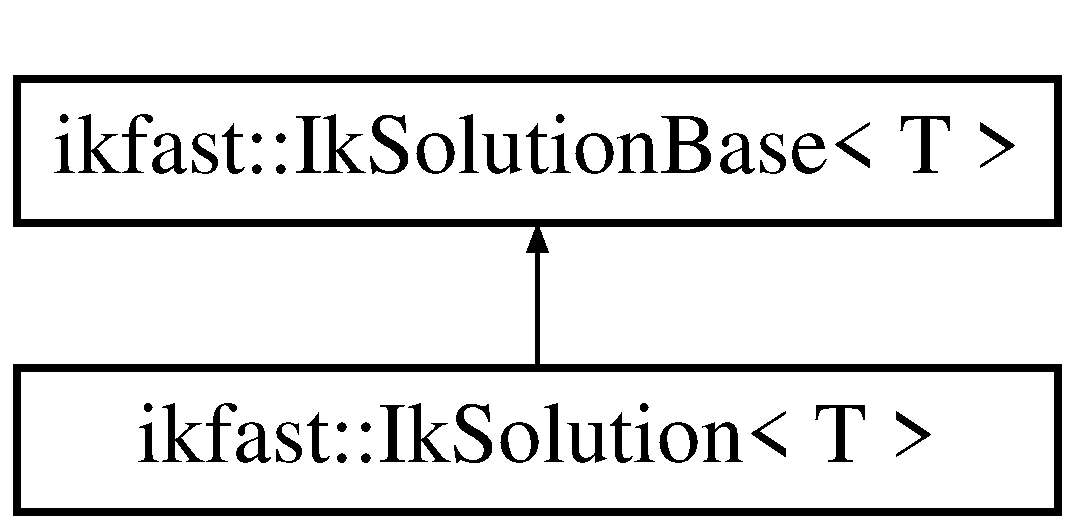
\includegraphics[height=2.000000cm]{classikfast_1_1IkSolution}
\end{center}
\end{figure}
\subsection*{Public Member Functions}
\begin{DoxyCompactItemize}
\item 
\hypertarget{classikfast_1_1IkSolution_a6b76af506a24ba4b78b1c9d3dc110a72}{{\bfseries Ik\-Solution} (const std\-::vector$<$ \hyperlink{classikfast_1_1IkSingleDOFSolutionBase}{Ik\-Single\-D\-O\-F\-Solution\-Base}$<$ T $>$ $>$ \&vinfos, const std\-::vector$<$ int $>$ \&vfree)}\label{classikfast_1_1IkSolution_a6b76af506a24ba4b78b1c9d3dc110a72}

\item 
virtual void \hyperlink{classikfast_1_1IkSolution_a197868105dffb498bec69c38318283a2}{Get\-Solution} (T $\ast$solution, const T $\ast$freevalues) const 
\begin{DoxyCompactList}\small\item\em gets a concrete solution \end{DoxyCompactList}\item 
\hypertarget{classikfast_1_1IkSolution_a56a7305f2111808478f85a43ecc5e6aa}{virtual void \hyperlink{classikfast_1_1IkSolution_a56a7305f2111808478f85a43ecc5e6aa}{Get\-Solution} (std\-::vector$<$ T $>$ \&solution, const std\-::vector$<$ T $>$ \&freevalues) const }\label{classikfast_1_1IkSolution_a56a7305f2111808478f85a43ecc5e6aa}

\begin{DoxyCompactList}\small\item\em std\-::vector version of \hyperlink{classikfast_1_1IkSolution_a197868105dffb498bec69c38318283a2}{Get\-Solution} \end{DoxyCompactList}\item 
virtual const std\-::vector$<$ int $>$ \& \hyperlink{classikfast_1_1IkSolution_a31267c02ff31436b0bfe3672bcecce5e}{Get\-Free} () const 
\begin{DoxyCompactList}\small\item\em Gets the indices of the configuration space that have to be preset before a full solution can be returned. \end{DoxyCompactList}\item 
\hypertarget{classikfast_1_1IkSolution_a8d46fe7ed5a582f9ad3f4bfc86b41297}{virtual const int \hyperlink{classikfast_1_1IkSolution_a8d46fe7ed5a582f9ad3f4bfc86b41297}{Get\-D\-O\-F} () const }\label{classikfast_1_1IkSolution_a8d46fe7ed5a582f9ad3f4bfc86b41297}

\begin{DoxyCompactList}\small\item\em the dof of the solution \end{DoxyCompactList}\item 
\hypertarget{classikfast_1_1IkSolution_ad61847499fe76751629f70047f8b0a69}{virtual void {\bfseries Validate} () const }\label{classikfast_1_1IkSolution_ad61847499fe76751629f70047f8b0a69}

\item 
\hypertarget{classikfast_1_1IkSolution_ae6b77cab94b40369712a099cc21d42e8}{virtual void {\bfseries Get\-Solution\-Indices} (std\-::vector$<$ unsigned int $>$ \&v) const }\label{classikfast_1_1IkSolution_ae6b77cab94b40369712a099cc21d42e8}

\end{DoxyCompactItemize}
\subsection*{Public Attributes}
\begin{DoxyCompactItemize}
\item 
\hypertarget{classikfast_1_1IkSolution_ac1b4c9612cee58a2b98388454b1054d7}{std\-::vector\\*
$<$ \hyperlink{classikfast_1_1IkSingleDOFSolutionBase}{Ik\-Single\-D\-O\-F\-Solution\-Base}$<$ T $>$ $>$ \hyperlink{classikfast_1_1IkSolution_ac1b4c9612cee58a2b98388454b1054d7}{\-\_\-vbasesol}}\label{classikfast_1_1IkSolution_ac1b4c9612cee58a2b98388454b1054d7}

\begin{DoxyCompactList}\small\item\em solution and their offsets if joints are mimiced \end{DoxyCompactList}\item 
\hypertarget{classikfast_1_1IkSolution_a3c552543a66e39e127bed5a5c085b1bb}{std\-::vector$<$ int $>$ {\bfseries \-\_\-vfree}}\label{classikfast_1_1IkSolution_a3c552543a66e39e127bed5a5c085b1bb}

\end{DoxyCompactItemize}


\subsection{Detailed Description}
\subsubsection*{template$<$typename T$>$class ikfast\-::\-Ik\-Solution$<$ T $>$}

Default implementation of \hyperlink{classikfast_1_1IkSolutionBase}{Ik\-Solution\-Base}. 

\subsection{Member Function Documentation}
\hypertarget{classikfast_1_1IkSolution_a31267c02ff31436b0bfe3672bcecce5e}{\index{ikfast\-::\-Ik\-Solution@{ikfast\-::\-Ik\-Solution}!Get\-Free@{Get\-Free}}
\index{Get\-Free@{Get\-Free}!ikfast::IkSolution@{ikfast\-::\-Ik\-Solution}}
\subsubsection[{Get\-Free}]{\setlength{\rightskip}{0pt plus 5cm}template$<$typename T $>$ virtual const std\-::vector$<$int$>$\& {\bf ikfast\-::\-Ik\-Solution}$<$ T $>$\-::Get\-Free (
\begin{DoxyParamCaption}
{}
\end{DoxyParamCaption}
) const\hspace{0.3cm}{\ttfamily [inline]}, {\ttfamily [virtual]}}}\label{classikfast_1_1IkSolution_a31267c02ff31436b0bfe3672bcecce5e}


Gets the indices of the configuration space that have to be preset before a full solution can be returned. 

0 always points to the first value accepted by the ik function. \begin{DoxyReturn}{Returns}
vector of indices indicating the free parameters 
\end{DoxyReturn}


Implements \hyperlink{classikfast_1_1IkSolutionBase_a2693ede66be937b7c4c1c949284282ca}{ikfast\-::\-Ik\-Solution\-Base$<$ T $>$}.


\begin{DoxyCode}
184                                                   \{
185         \textcolor{keywordflow}{return} \_vfree;
186     \}
\end{DoxyCode}
\hypertarget{classikfast_1_1IkSolution_a197868105dffb498bec69c38318283a2}{\index{ikfast\-::\-Ik\-Solution@{ikfast\-::\-Ik\-Solution}!Get\-Solution@{Get\-Solution}}
\index{Get\-Solution@{Get\-Solution}!ikfast::IkSolution@{ikfast\-::\-Ik\-Solution}}
\subsubsection[{Get\-Solution}]{\setlength{\rightskip}{0pt plus 5cm}template$<$typename T $>$ virtual void {\bf ikfast\-::\-Ik\-Solution}$<$ T $>$\-::Get\-Solution (
\begin{DoxyParamCaption}
\item[{T $\ast$}]{solution, }
\item[{const T $\ast$}]{freevalues}
\end{DoxyParamCaption}
) const\hspace{0.3cm}{\ttfamily [inline]}, {\ttfamily [virtual]}}}\label{classikfast_1_1IkSolution_a197868105dffb498bec69c38318283a2}


gets a concrete solution 


\begin{DoxyParams}[1]{Parameters}
\mbox{\tt out}  & {\em solution} & the result \\
\hline
\mbox{\tt in}  & {\em freevalues} & values for the free parameters  Get\-Free \\
\hline
\end{DoxyParams}


Implements \hyperlink{classikfast_1_1IkSolutionBase_a9405530feb49f12f56c3175e7150c66f}{ikfast\-::\-Ik\-Solution\-Base$<$ T $>$}.


\begin{DoxyCode}
163                                                                      \{
164         \textcolor{keywordflow}{for}(std::size\_t i = 0; i < \hyperlink{classikfast_1_1IkSolution_ac1b4c9612cee58a2b98388454b1054d7}{\_vbasesol}.size(); ++i) \{
165             \textcolor{keywordflow}{if}( \hyperlink{classikfast_1_1IkSolution_ac1b4c9612cee58a2b98388454b1054d7}{\_vbasesol}[i].freeind < 0 )
166                 solution[i] = \hyperlink{classikfast_1_1IkSolution_ac1b4c9612cee58a2b98388454b1054d7}{\_vbasesol}[i].foffset;
167             \textcolor{keywordflow}{else} \{
168                 solution[i] = freevalues[\hyperlink{classikfast_1_1IkSolution_ac1b4c9612cee58a2b98388454b1054d7}{\_vbasesol}[i].freeind]*
      \hyperlink{classikfast_1_1IkSolution_ac1b4c9612cee58a2b98388454b1054d7}{\_vbasesol}[i].fmul + \hyperlink{classikfast_1_1IkSolution_ac1b4c9612cee58a2b98388454b1054d7}{\_vbasesol}[i].foffset;
169                 \textcolor{keywordflow}{if}( solution[i] > T(3.14159265358979) ) \{
170                     solution[i] -= T(6.28318530717959);
171                 \}
172                 \textcolor{keywordflow}{else} \textcolor{keywordflow}{if}( solution[i] < T(-3.14159265358979) ) \{
173                     solution[i] += T(6.28318530717959);
174                 \}
175             \}
176         \}
177     \}
\end{DoxyCode}


The documentation for this class was generated from the following file\-:\begin{DoxyCompactItemize}
\item 
inc/\hyperlink{ikfast_8h}{ikfast.\-h}\end{DoxyCompactItemize}

\hypertarget{classikfast_1_1IkSolutionBase}{\section{ikfast\-:\-:Ik\-Solution\-Base$<$ T $>$ Class Template Reference}
\label{classikfast_1_1IkSolutionBase}\index{ikfast\-::\-Ik\-Solution\-Base$<$ T $>$@{ikfast\-::\-Ik\-Solution\-Base$<$ T $>$}}
}


The discrete solutions are returned in this structure.  




{\ttfamily \#include $<$ikfast.\-h$>$}

Inheritance diagram for ikfast\-:\-:Ik\-Solution\-Base$<$ T $>$\-:\begin{figure}[H]
\begin{center}
\leavevmode
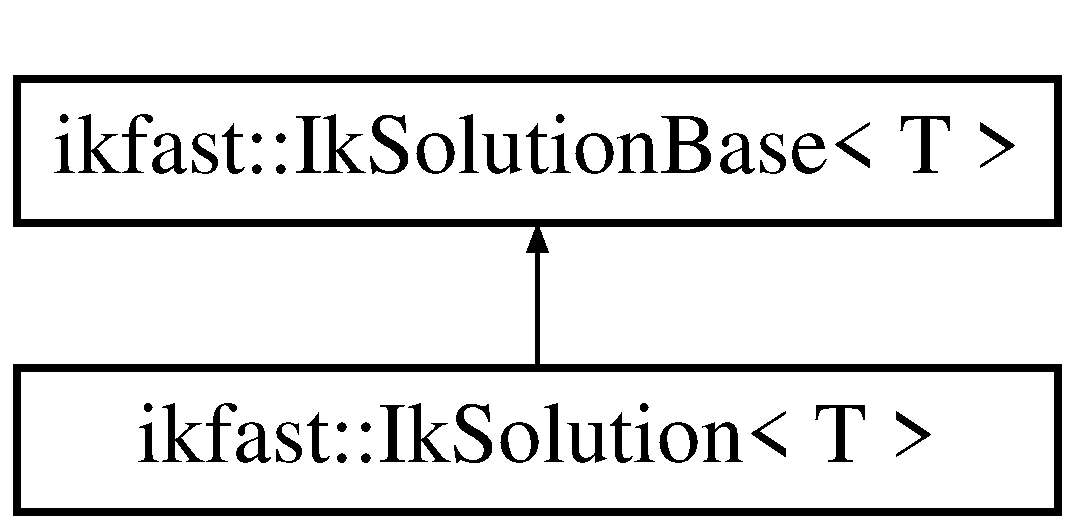
\includegraphics[height=2.000000cm]{classikfast_1_1IkSolutionBase}
\end{center}
\end{figure}
\subsection*{Public Member Functions}
\begin{DoxyCompactItemize}
\item 
virtual void \hyperlink{classikfast_1_1IkSolutionBase_a9405530feb49f12f56c3175e7150c66f}{Get\-Solution} (T $\ast$solution, const T $\ast$freevalues) const =0
\begin{DoxyCompactList}\small\item\em gets a concrete solution \end{DoxyCompactList}\item 
\hypertarget{classikfast_1_1IkSolutionBase_a2b558f7a29be0868cff3e81fbd9594c4}{virtual void \hyperlink{classikfast_1_1IkSolutionBase_a2b558f7a29be0868cff3e81fbd9594c4}{Get\-Solution} (std\-::vector$<$ T $>$ \&solution, const std\-::vector$<$ T $>$ \&freevalues) const }\label{classikfast_1_1IkSolutionBase_a2b558f7a29be0868cff3e81fbd9594c4}

\begin{DoxyCompactList}\small\item\em std\-::vector version of \hyperlink{classikfast_1_1IkSolutionBase_a9405530feb49f12f56c3175e7150c66f}{Get\-Solution} \end{DoxyCompactList}\item 
virtual const std\-::vector$<$ int $>$ \& \hyperlink{classikfast_1_1IkSolutionBase_a2693ede66be937b7c4c1c949284282ca}{Get\-Free} () const =0
\begin{DoxyCompactList}\small\item\em Gets the indices of the configuration space that have to be preset before a full solution can be returned. \end{DoxyCompactList}\item 
\hypertarget{classikfast_1_1IkSolutionBase_aac54f54aa69b27991651b0ba2a21208c}{virtual const int \hyperlink{classikfast_1_1IkSolutionBase_aac54f54aa69b27991651b0ba2a21208c}{Get\-D\-O\-F} () const =0}\label{classikfast_1_1IkSolutionBase_aac54f54aa69b27991651b0ba2a21208c}

\begin{DoxyCompactList}\small\item\em the dof of the solution \end{DoxyCompactList}\end{DoxyCompactItemize}


\subsection{Detailed Description}
\subsubsection*{template$<$typename T$>$class ikfast\-::\-Ik\-Solution\-Base$<$ T $>$}

The discrete solutions are returned in this structure. 

Sometimes the joint axes of the robot can align allowing an infinite number of solutions. Stores all these solutions in the form of free variables that the user has to set when querying the solution. Its prototype is\-: 

\subsection{Member Function Documentation}
\hypertarget{classikfast_1_1IkSolutionBase_a2693ede66be937b7c4c1c949284282ca}{\index{ikfast\-::\-Ik\-Solution\-Base@{ikfast\-::\-Ik\-Solution\-Base}!Get\-Free@{Get\-Free}}
\index{Get\-Free@{Get\-Free}!ikfast::IkSolutionBase@{ikfast\-::\-Ik\-Solution\-Base}}
\subsubsection[{Get\-Free}]{\setlength{\rightskip}{0pt plus 5cm}template$<$typename T $>$ virtual const std\-::vector$<$int$>$\& {\bf ikfast\-::\-Ik\-Solution\-Base}$<$ T $>$\-::Get\-Free (
\begin{DoxyParamCaption}
{}
\end{DoxyParamCaption}
) const\hspace{0.3cm}{\ttfamily [pure virtual]}}}\label{classikfast_1_1IkSolutionBase_a2693ede66be937b7c4c1c949284282ca}


Gets the indices of the configuration space that have to be preset before a full solution can be returned. 

0 always points to the first value accepted by the ik function. \begin{DoxyReturn}{Returns}
vector of indices indicating the free parameters 
\end{DoxyReturn}


Implemented in \hyperlink{classikfast_1_1IkSolution_a31267c02ff31436b0bfe3672bcecce5e}{ikfast\-::\-Ik\-Solution$<$ T $>$}.

\hypertarget{classikfast_1_1IkSolutionBase_a9405530feb49f12f56c3175e7150c66f}{\index{ikfast\-::\-Ik\-Solution\-Base@{ikfast\-::\-Ik\-Solution\-Base}!Get\-Solution@{Get\-Solution}}
\index{Get\-Solution@{Get\-Solution}!ikfast::IkSolutionBase@{ikfast\-::\-Ik\-Solution\-Base}}
\subsubsection[{Get\-Solution}]{\setlength{\rightskip}{0pt plus 5cm}template$<$typename T $>$ virtual void {\bf ikfast\-::\-Ik\-Solution\-Base}$<$ T $>$\-::Get\-Solution (
\begin{DoxyParamCaption}
\item[{T $\ast$}]{solution, }
\item[{const T $\ast$}]{freevalues}
\end{DoxyParamCaption}
) const\hspace{0.3cm}{\ttfamily [pure virtual]}}}\label{classikfast_1_1IkSolutionBase_a9405530feb49f12f56c3175e7150c66f}


gets a concrete solution 


\begin{DoxyParams}[1]{Parameters}
\mbox{\tt out}  & {\em solution} & the result \\
\hline
\mbox{\tt in}  & {\em freevalues} & values for the free parameters  Get\-Free \\
\hline
\end{DoxyParams}


Implemented in \hyperlink{classikfast_1_1IkSolution_a197868105dffb498bec69c38318283a2}{ikfast\-::\-Ik\-Solution$<$ T $>$}.



The documentation for this class was generated from the following file\-:\begin{DoxyCompactItemize}
\item 
inc/\hyperlink{ikfast_8h}{ikfast.\-h}\end{DoxyCompactItemize}

\hypertarget{classikfast_1_1IkSolutionList}{\section{ikfast\-:\-:Ik\-Solution\-List$<$ T $>$ Class Template Reference}
\label{classikfast_1_1IkSolutionList}\index{ikfast\-::\-Ik\-Solution\-List$<$ T $>$@{ikfast\-::\-Ik\-Solution\-List$<$ T $>$}}
}


Default implementation of \hyperlink{classikfast_1_1IkSolutionListBase}{Ik\-Solution\-List\-Base}.  




{\ttfamily \#include $<$ikfast.\-h$>$}

Inheritance diagram for ikfast\-:\-:Ik\-Solution\-List$<$ T $>$\-:\begin{figure}[H]
\begin{center}
\leavevmode
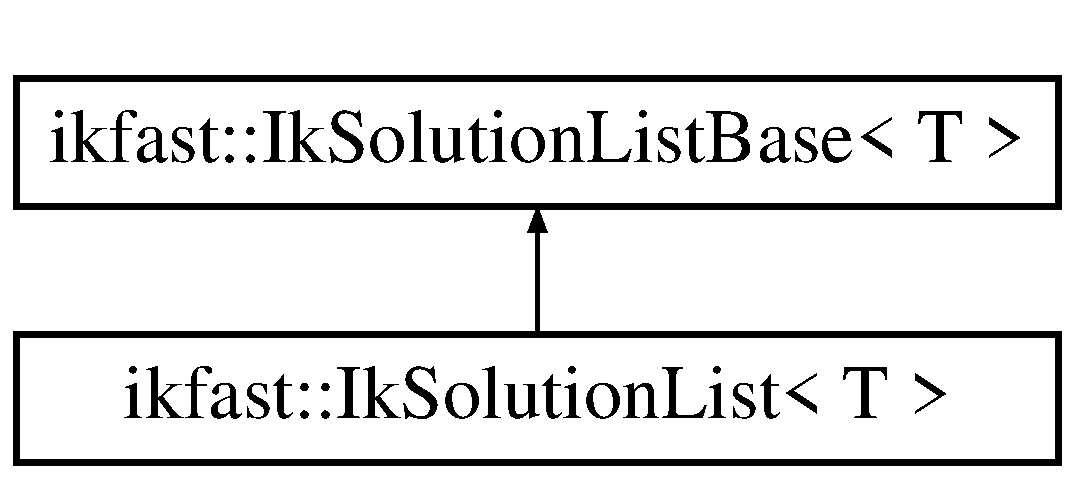
\includegraphics[height=2.000000cm]{classikfast_1_1IkSolutionList}
\end{center}
\end{figure}
\subsection*{Public Member Functions}
\begin{DoxyCompactItemize}
\item 
virtual size\-\_\-t \hyperlink{classikfast_1_1IkSolutionList_ac0a503b13e68403e7b2d92afd4c28a7b}{Add\-Solution} (const std\-::vector$<$ \hyperlink{classikfast_1_1IkSingleDOFSolutionBase}{Ik\-Single\-D\-O\-F\-Solution\-Base}$<$ T $>$ $>$ \&vinfos, const std\-::vector$<$ int $>$ \&vfree)
\begin{DoxyCompactList}\small\item\em add one solution and return its index for later retrieval \end{DoxyCompactList}\item 
\hypertarget{classikfast_1_1IkSolutionList_ab2840cca4cea5547d684907047d38bba}{virtual const \hyperlink{classikfast_1_1IkSolutionBase}{Ik\-Solution\-Base}$<$ T $>$ \& \hyperlink{classikfast_1_1IkSolutionList_ab2840cca4cea5547d684907047d38bba}{Get\-Solution} (size\-\_\-t index) const }\label{classikfast_1_1IkSolutionList_ab2840cca4cea5547d684907047d38bba}

\begin{DoxyCompactList}\small\item\em returns the solution pointer \end{DoxyCompactList}\item 
\hypertarget{classikfast_1_1IkSolutionList_a4508235ea7738ee067d6525a34362567}{virtual size\-\_\-t \hyperlink{classikfast_1_1IkSolutionList_a4508235ea7738ee067d6525a34362567}{Get\-Num\-Solutions} () const }\label{classikfast_1_1IkSolutionList_a4508235ea7738ee067d6525a34362567}

\begin{DoxyCompactList}\small\item\em returns the number of solutions stored \end{DoxyCompactList}\item 
\hypertarget{classikfast_1_1IkSolutionList_ae341a33d5aee644cac867e3edd2a9916}{virtual void \hyperlink{classikfast_1_1IkSolutionList_ae341a33d5aee644cac867e3edd2a9916}{Clear} ()}\label{classikfast_1_1IkSolutionList_ae341a33d5aee644cac867e3edd2a9916}

\begin{DoxyCompactList}\small\item\em clears all current solutions, note that any memory addresses returned from \hyperlink{classikfast_1_1IkSolutionList_ab2840cca4cea5547d684907047d38bba}{Get\-Solution} will be invalidated. \end{DoxyCompactList}\end{DoxyCompactItemize}
\subsection*{Protected Attributes}
\begin{DoxyCompactItemize}
\item 
\hypertarget{classikfast_1_1IkSolutionList_acaba262a6f62eee0620b6f190dbbe185}{std\-::list$<$ \hyperlink{classikfast_1_1IkSolution}{Ik\-Solution}$<$ T $>$ $>$ {\bfseries \-\_\-listsolutions}}\label{classikfast_1_1IkSolutionList_acaba262a6f62eee0620b6f190dbbe185}

\end{DoxyCompactItemize}


\subsection{Detailed Description}
\subsubsection*{template$<$typename T$>$class ikfast\-::\-Ik\-Solution\-List$<$ T $>$}

Default implementation of \hyperlink{classikfast_1_1IkSolutionListBase}{Ik\-Solution\-List\-Base}. 

\subsection{Member Function Documentation}
\hypertarget{classikfast_1_1IkSolutionList_ac0a503b13e68403e7b2d92afd4c28a7b}{\index{ikfast\-::\-Ik\-Solution\-List@{ikfast\-::\-Ik\-Solution\-List}!Add\-Solution@{Add\-Solution}}
\index{Add\-Solution@{Add\-Solution}!ikfast::IkSolutionList@{ikfast\-::\-Ik\-Solution\-List}}
\subsubsection[{Add\-Solution}]{\setlength{\rightskip}{0pt plus 5cm}template$<$typename T $>$ virtual size\-\_\-t {\bf ikfast\-::\-Ik\-Solution\-List}$<$ T $>$\-::Add\-Solution (
\begin{DoxyParamCaption}
\item[{const std\-::vector$<$ {\bf Ik\-Single\-D\-O\-F\-Solution\-Base}$<$ T $>$ $>$ \&}]{vinfos, }
\item[{const std\-::vector$<$ int $>$ \&}]{vfree}
\end{DoxyParamCaption}
)\hspace{0.3cm}{\ttfamily [inline]}, {\ttfamily [virtual]}}}\label{classikfast_1_1IkSolutionList_ac0a503b13e68403e7b2d92afd4c28a7b}


add one solution and return its index for later retrieval 


\begin{DoxyParams}{Parameters}
{\em vinfos} & Solution data for each degree of freedom of the manipulator \\
\hline
{\em vfree} & If the solution represents an infinite space, holds free parameters of the solution that users can freely set. The indices are of the configuration that the I\-K solver accepts rather than the entire robot, ie 0 points to the first value accepted. \\
\hline
\end{DoxyParams}


Implements \hyperlink{classikfast_1_1IkSolutionListBase_a9d862f550472c2fa15189946b12222bf}{ikfast\-::\-Ik\-Solution\-List\-Base$<$ T $>$}.


\begin{DoxyCode}
243     \{
244         \textcolor{keywordtype}{size\_t} index = \_listsolutions.size();
245         \_listsolutions.push\_back(IkSolution<T>(vinfos,vfree));
246         \textcolor{keywordflow}{return} index;
247     \}
\end{DoxyCode}


The documentation for this class was generated from the following file\-:\begin{DoxyCompactItemize}
\item 
inc/\hyperlink{ikfast_8h}{ikfast.\-h}\end{DoxyCompactItemize}

\hypertarget{classikfast_1_1IkSolutionListBase}{\section{ikfast\-:\-:Ik\-Solution\-List\-Base$<$ T $>$ Class Template Reference}
\label{classikfast_1_1IkSolutionListBase}\index{ikfast\-::\-Ik\-Solution\-List\-Base$<$ T $>$@{ikfast\-::\-Ik\-Solution\-List\-Base$<$ T $>$}}
}


manages all the solutions  




{\ttfamily \#include $<$ikfast.\-h$>$}

Inheritance diagram for ikfast\-:\-:Ik\-Solution\-List\-Base$<$ T $>$\-:\begin{figure}[H]
\begin{center}
\leavevmode
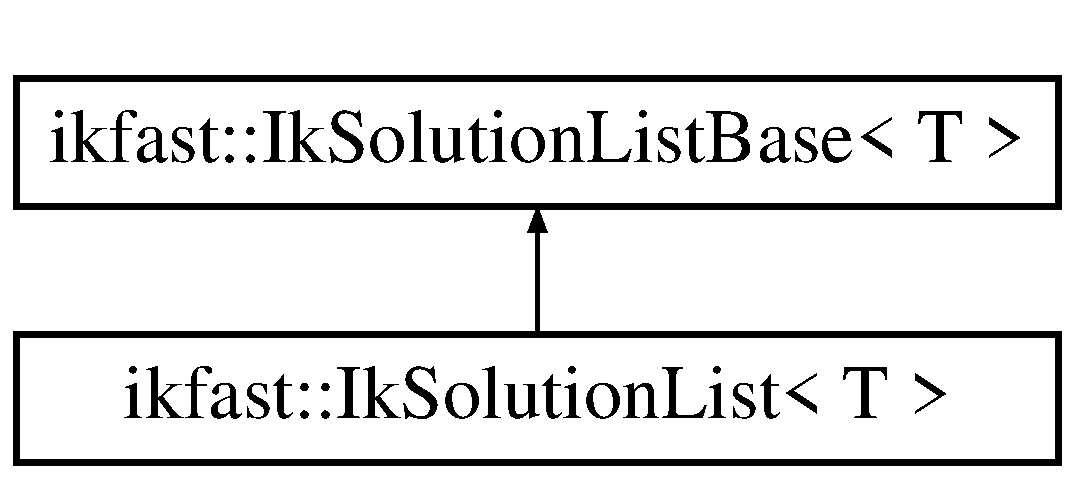
\includegraphics[height=2.000000cm]{classikfast_1_1IkSolutionListBase}
\end{center}
\end{figure}
\subsection*{Public Member Functions}
\begin{DoxyCompactItemize}
\item 
virtual size\-\_\-t \hyperlink{classikfast_1_1IkSolutionListBase_a9d862f550472c2fa15189946b12222bf}{Add\-Solution} (const std\-::vector$<$ \hyperlink{classikfast_1_1IkSingleDOFSolutionBase}{Ik\-Single\-D\-O\-F\-Solution\-Base}$<$ T $>$ $>$ \&vinfos, const std\-::vector$<$ int $>$ \&vfree)=0
\begin{DoxyCompactList}\small\item\em add one solution and return its index for later retrieval \end{DoxyCompactList}\item 
\hypertarget{classikfast_1_1IkSolutionListBase_a540d8c85b5be635ea671ef7ddc0eb9c0}{virtual const \hyperlink{classikfast_1_1IkSolutionBase}{Ik\-Solution\-Base}$<$ T $>$ \& \hyperlink{classikfast_1_1IkSolutionListBase_a540d8c85b5be635ea671ef7ddc0eb9c0}{Get\-Solution} (size\-\_\-t index) const =0}\label{classikfast_1_1IkSolutionListBase_a540d8c85b5be635ea671ef7ddc0eb9c0}

\begin{DoxyCompactList}\small\item\em returns the solution pointer \end{DoxyCompactList}\item 
\hypertarget{classikfast_1_1IkSolutionListBase_a5f4a2191825f1d2aad3468daf94d575f}{virtual size\-\_\-t \hyperlink{classikfast_1_1IkSolutionListBase_a5f4a2191825f1d2aad3468daf94d575f}{Get\-Num\-Solutions} () const =0}\label{classikfast_1_1IkSolutionListBase_a5f4a2191825f1d2aad3468daf94d575f}

\begin{DoxyCompactList}\small\item\em returns the number of solutions stored \end{DoxyCompactList}\item 
\hypertarget{classikfast_1_1IkSolutionListBase_a9940fe21cfa0a67c1a21a672696c5cb5}{virtual void \hyperlink{classikfast_1_1IkSolutionListBase_a9940fe21cfa0a67c1a21a672696c5cb5}{Clear} ()=0}\label{classikfast_1_1IkSolutionListBase_a9940fe21cfa0a67c1a21a672696c5cb5}

\begin{DoxyCompactList}\small\item\em clears all current solutions, note that any memory addresses returned from \hyperlink{classikfast_1_1IkSolutionListBase_a540d8c85b5be635ea671ef7ddc0eb9c0}{Get\-Solution} will be invalidated. \end{DoxyCompactList}\end{DoxyCompactItemize}


\subsection{Detailed Description}
\subsubsection*{template$<$typename T$>$class ikfast\-::\-Ik\-Solution\-List\-Base$<$ T $>$}

manages all the solutions 

\subsection{Member Function Documentation}
\hypertarget{classikfast_1_1IkSolutionListBase_a9d862f550472c2fa15189946b12222bf}{\index{ikfast\-::\-Ik\-Solution\-List\-Base@{ikfast\-::\-Ik\-Solution\-List\-Base}!Add\-Solution@{Add\-Solution}}
\index{Add\-Solution@{Add\-Solution}!ikfast::IkSolutionListBase@{ikfast\-::\-Ik\-Solution\-List\-Base}}
\subsubsection[{Add\-Solution}]{\setlength{\rightskip}{0pt plus 5cm}template$<$typename T$>$ virtual size\-\_\-t {\bf ikfast\-::\-Ik\-Solution\-List\-Base}$<$ T $>$\-::Add\-Solution (
\begin{DoxyParamCaption}
\item[{const std\-::vector$<$ {\bf Ik\-Single\-D\-O\-F\-Solution\-Base}$<$ T $>$ $>$ \&}]{vinfos, }
\item[{const std\-::vector$<$ int $>$ \&}]{vfree}
\end{DoxyParamCaption}
)\hspace{0.3cm}{\ttfamily [pure virtual]}}}\label{classikfast_1_1IkSolutionListBase_a9d862f550472c2fa15189946b12222bf}


add one solution and return its index for later retrieval 


\begin{DoxyParams}{Parameters}
{\em vinfos} & Solution data for each degree of freedom of the manipulator \\
\hline
{\em vfree} & If the solution represents an infinite space, holds free parameters of the solution that users can freely set. The indices are of the configuration that the I\-K solver accepts rather than the entire robot, ie 0 points to the first value accepted. \\
\hline
\end{DoxyParams}


Implemented in \hyperlink{classikfast_1_1IkSolutionList_ac0a503b13e68403e7b2d92afd4c28a7b}{ikfast\-::\-Ik\-Solution\-List$<$ T $>$}.



The documentation for this class was generated from the following file\-:\begin{DoxyCompactItemize}
\item 
inc/\hyperlink{ikfast_8h}{ikfast.\-h}\end{DoxyCompactItemize}

\hypertarget{classIKSolver}{\section{I\-K\-Solver Class Reference}
\label{classIKSolver}\index{I\-K\-Solver@{I\-K\-Solver}}
}
\subsection*{Public Member Functions}
\begin{DoxyCompactItemize}
\item 
\hypertarget{classIKSolver_ac0195e291bed491b4cb6a68db8199b55}{bool {\bfseries Compute\-Ik} (const Ik\-Real $\ast$eetrans, const Ik\-Real $\ast$eerot, const Ik\-Real $\ast$pfree, \hyperlink{classikfast_1_1IkSolutionListBase}{Ik\-Solution\-List\-Base}$<$ Ik\-Real $>$ \&solutions)}\label{classIKSolver_ac0195e291bed491b4cb6a68db8199b55}

\item 
\hypertarget{classIKSolver_a5052994576b6519164e978e851c3237c}{void {\bfseries innerfn} (\hyperlink{classikfast_1_1IkSolutionListBase}{Ik\-Solution\-List\-Base}$<$ Ik\-Real $>$ \&solutions)}\label{classIKSolver_a5052994576b6519164e978e851c3237c}

\end{DoxyCompactItemize}
\subsection*{Static Public Member Functions}
\begin{DoxyCompactItemize}
\item 
\hypertarget{classIKSolver_abecf6ea0c9933661bd0f3caeb0561881}{static bool {\bfseries checkconsistency8} (const Ik\-Real $\ast$Breal)}\label{classIKSolver_abecf6ea0c9933661bd0f3caeb0561881}

\item 
static void \hyperlink{classIKSolver_a058e681da2d434157aad2abbbce6bf02}{solvedialyticpoly8qep} (const Ik\-Real $\ast$matcoeffs, Ik\-Real $\ast$rawroots, int \&numroots)
\begin{DoxyCompactList}\small\item\em Solve the det Ax$^\wedge$2+\-Bx+\-C = 0 problem using the Manocha and Canny method (1994) \end{DoxyCompactList}\end{DoxyCompactItemize}
\subsection*{Public Attributes}
\begin{DoxyCompactItemize}
\item 
\hypertarget{classIKSolver_a57f10792b61e342bc910311172b36488}{Ik\-Real {\bfseries j0}}\label{classIKSolver_a57f10792b61e342bc910311172b36488}

\item 
\hypertarget{classIKSolver_aa3c0bd74bcf87573ce608d8039408526}{Ik\-Real {\bfseries cj0}}\label{classIKSolver_aa3c0bd74bcf87573ce608d8039408526}

\item 
\hypertarget{classIKSolver_a791e2437d1fc1b568b213b0388f97d0a}{Ik\-Real {\bfseries sj0}}\label{classIKSolver_a791e2437d1fc1b568b213b0388f97d0a}

\item 
\hypertarget{classIKSolver_af29aefe604a6957a573f5532a0ae0924}{Ik\-Real {\bfseries htj0}}\label{classIKSolver_af29aefe604a6957a573f5532a0ae0924}

\item 
\hypertarget{classIKSolver_a7e5b52eca8716ef85d3e857c5c6a0664}{Ik\-Real {\bfseries j0mul}}\label{classIKSolver_a7e5b52eca8716ef85d3e857c5c6a0664}

\item 
\hypertarget{classIKSolver_abce606fc49166277524525eadfe47f1a}{Ik\-Real {\bfseries j1}}\label{classIKSolver_abce606fc49166277524525eadfe47f1a}

\item 
\hypertarget{classIKSolver_a2eff4800151517f5c649cb948bad8326}{Ik\-Real {\bfseries cj1}}\label{classIKSolver_a2eff4800151517f5c649cb948bad8326}

\item 
\hypertarget{classIKSolver_a0d7c3270795003a7947ae93ba90b8335}{Ik\-Real {\bfseries sj1}}\label{classIKSolver_a0d7c3270795003a7947ae93ba90b8335}

\item 
\hypertarget{classIKSolver_aa12be6bab85a8ca6c8c74c0cb5e92cf9}{Ik\-Real {\bfseries htj1}}\label{classIKSolver_aa12be6bab85a8ca6c8c74c0cb5e92cf9}

\item 
\hypertarget{classIKSolver_a8e666ee88199689ecabf3d3457d86bc2}{Ik\-Real {\bfseries j1mul}}\label{classIKSolver_a8e666ee88199689ecabf3d3457d86bc2}

\item 
\hypertarget{classIKSolver_a2059d93255027d204610a6818e5c45a6}{Ik\-Real {\bfseries j2}}\label{classIKSolver_a2059d93255027d204610a6818e5c45a6}

\item 
\hypertarget{classIKSolver_afae239eeaad5f0c027cd4837faa666a0}{Ik\-Real {\bfseries cj2}}\label{classIKSolver_afae239eeaad5f0c027cd4837faa666a0}

\item 
\hypertarget{classIKSolver_adbd68395fd872d5e9a13f3a787c1b0d9}{Ik\-Real {\bfseries sj2}}\label{classIKSolver_adbd68395fd872d5e9a13f3a787c1b0d9}

\item 
\hypertarget{classIKSolver_a33e07730a03291ee56912b371dc8268f}{Ik\-Real {\bfseries htj2}}\label{classIKSolver_a33e07730a03291ee56912b371dc8268f}

\item 
\hypertarget{classIKSolver_a293ea10271033383fd77c557befd11b4}{Ik\-Real {\bfseries j2mul}}\label{classIKSolver_a293ea10271033383fd77c557befd11b4}

\item 
\hypertarget{classIKSolver_adf5d1568dc258d51edc6430bf90ef09d}{Ik\-Real {\bfseries j3}}\label{classIKSolver_adf5d1568dc258d51edc6430bf90ef09d}

\item 
\hypertarget{classIKSolver_ae9b832aafcb4e3630a581c04b15d909b}{Ik\-Real {\bfseries cj3}}\label{classIKSolver_ae9b832aafcb4e3630a581c04b15d909b}

\item 
\hypertarget{classIKSolver_a6b8d826d394d3d04633e5542d023ee5b}{Ik\-Real {\bfseries sj3}}\label{classIKSolver_a6b8d826d394d3d04633e5542d023ee5b}

\item 
\hypertarget{classIKSolver_ab1194d4acb88c80eb7dd3c75a099dd97}{Ik\-Real {\bfseries htj3}}\label{classIKSolver_ab1194d4acb88c80eb7dd3c75a099dd97}

\item 
\hypertarget{classIKSolver_a827e1cab13ea3962046446651efec165}{Ik\-Real {\bfseries j3mul}}\label{classIKSolver_a827e1cab13ea3962046446651efec165}

\item 
\hypertarget{classIKSolver_a7f090894b4553ceda8b2fbe91a9d469c}{Ik\-Real {\bfseries j4}}\label{classIKSolver_a7f090894b4553ceda8b2fbe91a9d469c}

\item 
\hypertarget{classIKSolver_a43e7823ac1496d1210dda7b76a4e037a}{Ik\-Real {\bfseries cj4}}\label{classIKSolver_a43e7823ac1496d1210dda7b76a4e037a}

\item 
\hypertarget{classIKSolver_a5f90cdbcbc7633850cfaeb547c11437c}{Ik\-Real {\bfseries sj4}}\label{classIKSolver_a5f90cdbcbc7633850cfaeb547c11437c}

\item 
\hypertarget{classIKSolver_a84bea2670b08b33b5a24bb1d5d56d7ca}{Ik\-Real {\bfseries htj4}}\label{classIKSolver_a84bea2670b08b33b5a24bb1d5d56d7ca}

\item 
\hypertarget{classIKSolver_acde98d7f3aa628addf5ef056060431b5}{Ik\-Real {\bfseries j4mul}}\label{classIKSolver_acde98d7f3aa628addf5ef056060431b5}

\item 
\hypertarget{classIKSolver_af26fbd69409e20260ab54d0aadd88946}{Ik\-Real {\bfseries j5}}\label{classIKSolver_af26fbd69409e20260ab54d0aadd88946}

\item 
\hypertarget{classIKSolver_a8c1b8f7d311d0a7fa070d950b3e39e89}{Ik\-Real {\bfseries cj5}}\label{classIKSolver_a8c1b8f7d311d0a7fa070d950b3e39e89}

\item 
\hypertarget{classIKSolver_a81dcf624096262da947af3f71f4cc63f}{Ik\-Real {\bfseries sj5}}\label{classIKSolver_a81dcf624096262da947af3f71f4cc63f}

\item 
\hypertarget{classIKSolver_ab8ccb7ca78f4a53de4a520c9a37ccf57}{Ik\-Real {\bfseries htj5}}\label{classIKSolver_ab8ccb7ca78f4a53de4a520c9a37ccf57}

\item 
\hypertarget{classIKSolver_a4933a202f17f03ec1667024dd4351dba}{Ik\-Real {\bfseries j5mul}}\label{classIKSolver_a4933a202f17f03ec1667024dd4351dba}

\item 
\hypertarget{classIKSolver_a53a7eddb835224104838f523df53d07b}{Ik\-Real {\bfseries new\-\_\-r00}}\label{classIKSolver_a53a7eddb835224104838f523df53d07b}

\item 
\hypertarget{classIKSolver_abe2d67909dcd06df36369735b9eb44f6}{Ik\-Real {\bfseries r00}}\label{classIKSolver_abe2d67909dcd06df36369735b9eb44f6}

\item 
\hypertarget{classIKSolver_a6640ab19abf5f8d59d1f268be598b9d3}{Ik\-Real {\bfseries rxp0\-\_\-0}}\label{classIKSolver_a6640ab19abf5f8d59d1f268be598b9d3}

\item 
\hypertarget{classIKSolver_a7bd00cd06f08e563763e834ffd0f66ea}{Ik\-Real {\bfseries new\-\_\-r01}}\label{classIKSolver_a7bd00cd06f08e563763e834ffd0f66ea}

\item 
\hypertarget{classIKSolver_ac19d13d4cf04f8fa93f295b67115ba18}{Ik\-Real {\bfseries r01}}\label{classIKSolver_ac19d13d4cf04f8fa93f295b67115ba18}

\item 
\hypertarget{classIKSolver_ae74bd1bcaca3440377e9afa78f39dae4}{Ik\-Real {\bfseries rxp0\-\_\-1}}\label{classIKSolver_ae74bd1bcaca3440377e9afa78f39dae4}

\item 
\hypertarget{classIKSolver_a39f2dd1bfb92c6c5509f4da676748660}{Ik\-Real {\bfseries new\-\_\-r02}}\label{classIKSolver_a39f2dd1bfb92c6c5509f4da676748660}

\item 
\hypertarget{classIKSolver_a6b885721baf3d20900bffecc1830948c}{Ik\-Real {\bfseries r02}}\label{classIKSolver_a6b885721baf3d20900bffecc1830948c}

\item 
\hypertarget{classIKSolver_aac158b1a0802a655cea8a339b34abccc}{Ik\-Real {\bfseries rxp0\-\_\-2}}\label{classIKSolver_aac158b1a0802a655cea8a339b34abccc}

\item 
\hypertarget{classIKSolver_a72cd887c34e4383b4ef3040304af0e01}{Ik\-Real {\bfseries new\-\_\-r10}}\label{classIKSolver_a72cd887c34e4383b4ef3040304af0e01}

\item 
\hypertarget{classIKSolver_a9054607dadcc96f12938340f96ce36a7}{Ik\-Real {\bfseries r10}}\label{classIKSolver_a9054607dadcc96f12938340f96ce36a7}

\item 
\hypertarget{classIKSolver_ae937030fe14b9fde348e0bf4100c9227}{Ik\-Real {\bfseries rxp1\-\_\-0}}\label{classIKSolver_ae937030fe14b9fde348e0bf4100c9227}

\item 
\hypertarget{classIKSolver_a4be5ecd7788a4a85c7dea895f9a4d32d}{Ik\-Real {\bfseries new\-\_\-r11}}\label{classIKSolver_a4be5ecd7788a4a85c7dea895f9a4d32d}

\item 
\hypertarget{classIKSolver_ad6cd90376e76da6bb3cc127b69056aaf}{Ik\-Real {\bfseries r11}}\label{classIKSolver_ad6cd90376e76da6bb3cc127b69056aaf}

\item 
\hypertarget{classIKSolver_a44f8b2ca238030be5073d28ff9f177f2}{Ik\-Real {\bfseries rxp1\-\_\-1}}\label{classIKSolver_a44f8b2ca238030be5073d28ff9f177f2}

\item 
\hypertarget{classIKSolver_a41547ff920430005dd46456e44083339}{Ik\-Real {\bfseries new\-\_\-r12}}\label{classIKSolver_a41547ff920430005dd46456e44083339}

\item 
\hypertarget{classIKSolver_ac658d04515874d1703b952635030f056}{Ik\-Real {\bfseries r12}}\label{classIKSolver_ac658d04515874d1703b952635030f056}

\item 
\hypertarget{classIKSolver_a67b37120177c48213784f088ced73b2b}{Ik\-Real {\bfseries rxp1\-\_\-2}}\label{classIKSolver_a67b37120177c48213784f088ced73b2b}

\item 
\hypertarget{classIKSolver_a860c1c4839a01c2a122bd5a88bc31d94}{Ik\-Real {\bfseries new\-\_\-r20}}\label{classIKSolver_a860c1c4839a01c2a122bd5a88bc31d94}

\item 
\hypertarget{classIKSolver_a2369487211ddd441625e3e7aed869467}{Ik\-Real {\bfseries r20}}\label{classIKSolver_a2369487211ddd441625e3e7aed869467}

\item 
\hypertarget{classIKSolver_ae155800fbb031589ea32d44ff18aace4}{Ik\-Real {\bfseries rxp2\-\_\-0}}\label{classIKSolver_ae155800fbb031589ea32d44ff18aace4}

\item 
\hypertarget{classIKSolver_a36f6ab67d1d51e467319f83d2b768b9d}{Ik\-Real {\bfseries new\-\_\-r21}}\label{classIKSolver_a36f6ab67d1d51e467319f83d2b768b9d}

\item 
\hypertarget{classIKSolver_a6906e8cdc998ef02a6794b2ab68a40d8}{Ik\-Real {\bfseries r21}}\label{classIKSolver_a6906e8cdc998ef02a6794b2ab68a40d8}

\item 
\hypertarget{classIKSolver_ab8c1e5e0a1bf4fbe4e04ed6e2f1b83f8}{Ik\-Real {\bfseries rxp2\-\_\-1}}\label{classIKSolver_ab8c1e5e0a1bf4fbe4e04ed6e2f1b83f8}

\item 
\hypertarget{classIKSolver_a7789303f1a9a6b1f48d43d2b79c06226}{Ik\-Real {\bfseries new\-\_\-r22}}\label{classIKSolver_a7789303f1a9a6b1f48d43d2b79c06226}

\item 
\hypertarget{classIKSolver_a848e6f6f22463bd368632af25bf0b184}{Ik\-Real {\bfseries r22}}\label{classIKSolver_a848e6f6f22463bd368632af25bf0b184}

\item 
\hypertarget{classIKSolver_ac7dd398330c89e017a4907a335113c85}{Ik\-Real {\bfseries rxp2\-\_\-2}}\label{classIKSolver_ac7dd398330c89e017a4907a335113c85}

\item 
\hypertarget{classIKSolver_a81fbafdee3f4d7df5c82a4db80cb74d7}{Ik\-Real {\bfseries new\-\_\-px}}\label{classIKSolver_a81fbafdee3f4d7df5c82a4db80cb74d7}

\item 
\hypertarget{classIKSolver_a9d5c872c9a6b0b9fdc9ba4192763585f}{Ik\-Real {\bfseries px}}\label{classIKSolver_a9d5c872c9a6b0b9fdc9ba4192763585f}

\item 
\hypertarget{classIKSolver_a42126eca3b2110aff8451060bce76c9f}{Ik\-Real {\bfseries npx}}\label{classIKSolver_a42126eca3b2110aff8451060bce76c9f}

\item 
\hypertarget{classIKSolver_a92d9c8748e96823e08979ba79f215031}{Ik\-Real {\bfseries new\-\_\-py}}\label{classIKSolver_a92d9c8748e96823e08979ba79f215031}

\item 
\hypertarget{classIKSolver_a997924d324efb5f12e6642cb28ee1470}{Ik\-Real {\bfseries py}}\label{classIKSolver_a997924d324efb5f12e6642cb28ee1470}

\item 
\hypertarget{classIKSolver_ab79bcd5d003ba38f5c1926e35446d123}{Ik\-Real {\bfseries npy}}\label{classIKSolver_ab79bcd5d003ba38f5c1926e35446d123}

\item 
\hypertarget{classIKSolver_a298e74662237a8df2869e8ad8ec2d00e}{Ik\-Real {\bfseries new\-\_\-pz}}\label{classIKSolver_a298e74662237a8df2869e8ad8ec2d00e}

\item 
\hypertarget{classIKSolver_a34d107aa2bd31deda5da19b9c191f183}{Ik\-Real {\bfseries pz}}\label{classIKSolver_a34d107aa2bd31deda5da19b9c191f183}

\item 
\hypertarget{classIKSolver_ac5ba601bbc95efd9881f70ebf871c5c1}{Ik\-Real {\bfseries npz}}\label{classIKSolver_ac5ba601bbc95efd9881f70ebf871c5c1}

\item 
\hypertarget{classIKSolver_a2940190f4bac7e2fcd3d95503beb1a29}{Ik\-Real {\bfseries pp}}\label{classIKSolver_a2940190f4bac7e2fcd3d95503beb1a29}

\item 
\hypertarget{classIKSolver_ae0fdf96e14e42d408bc5e16580c81100}{unsigned char {\bfseries \-\_\-ij0} \mbox{[}2\mbox{]}}\label{classIKSolver_ae0fdf96e14e42d408bc5e16580c81100}

\item 
\hypertarget{classIKSolver_ac2fb0a00657f58a0bc49485454ddd914}{unsigned char {\bfseries \-\_\-nj0}}\label{classIKSolver_ac2fb0a00657f58a0bc49485454ddd914}

\item 
\hypertarget{classIKSolver_a66a0610cba0da00e09deda3c72e3909f}{unsigned char {\bfseries \-\_\-ij1} \mbox{[}2\mbox{]}}\label{classIKSolver_a66a0610cba0da00e09deda3c72e3909f}

\item 
\hypertarget{classIKSolver_a38f5fb04f76ea095f6835eb767de1bbb}{unsigned char {\bfseries \-\_\-nj1}}\label{classIKSolver_a38f5fb04f76ea095f6835eb767de1bbb}

\item 
\hypertarget{classIKSolver_aff0b7815729d44c5decbef316763d45f}{unsigned char {\bfseries \-\_\-ij2} \mbox{[}2\mbox{]}}\label{classIKSolver_aff0b7815729d44c5decbef316763d45f}

\item 
\hypertarget{classIKSolver_aac13220157c526f065b9f655b4a5cb7f}{unsigned char {\bfseries \-\_\-nj2}}\label{classIKSolver_aac13220157c526f065b9f655b4a5cb7f}

\item 
\hypertarget{classIKSolver_a4e65e7d6f429bdc4ad9146bda1b48712}{unsigned char {\bfseries \-\_\-ij3} \mbox{[}2\mbox{]}}\label{classIKSolver_a4e65e7d6f429bdc4ad9146bda1b48712}

\item 
\hypertarget{classIKSolver_a19d64b2e1f7c33b7492420d74ff280a0}{unsigned char {\bfseries \-\_\-nj3}}\label{classIKSolver_a19d64b2e1f7c33b7492420d74ff280a0}

\item 
\hypertarget{classIKSolver_a0b552c60bc1dd705f67a32cb3f03b738}{unsigned char {\bfseries \-\_\-ij4} \mbox{[}2\mbox{]}}\label{classIKSolver_a0b552c60bc1dd705f67a32cb3f03b738}

\item 
\hypertarget{classIKSolver_af4a3d8d26ff3a7cbf3ebbe8c8258f12c}{unsigned char {\bfseries \-\_\-nj4}}\label{classIKSolver_af4a3d8d26ff3a7cbf3ebbe8c8258f12c}

\item 
\hypertarget{classIKSolver_a19d1dfd6307ab991ba52a2508ca88ab9}{unsigned char {\bfseries \-\_\-ij5} \mbox{[}2\mbox{]}}\label{classIKSolver_a19d1dfd6307ab991ba52a2508ca88ab9}

\item 
\hypertarget{classIKSolver_aaa811fe7438ac359598271dc80f55ea7}{unsigned char {\bfseries \-\_\-nj5}}\label{classIKSolver_aaa811fe7438ac359598271dc80f55ea7}

\item 
\hypertarget{classIKSolver_a793dbaa888ed31ea892028f3da3b6251}{Ik\-Real {\bfseries j100}}\label{classIKSolver_a793dbaa888ed31ea892028f3da3b6251}

\item 
\hypertarget{classIKSolver_aff9b55d101572e59a2b2ff7255401883}{Ik\-Real {\bfseries cj100}}\label{classIKSolver_aff9b55d101572e59a2b2ff7255401883}

\item 
\hypertarget{classIKSolver_a481a9e5ad8adad9c244a5a1a8bca8124}{Ik\-Real {\bfseries sj100}}\label{classIKSolver_a481a9e5ad8adad9c244a5a1a8bca8124}

\item 
\hypertarget{classIKSolver_a532f95a61a95105a0d54bc0d480f8a1c}{unsigned char {\bfseries \-\_\-ij100} \mbox{[}2\mbox{]}}\label{classIKSolver_a532f95a61a95105a0d54bc0d480f8a1c}

\item 
\hypertarget{classIKSolver_ae2e2e25e523459bc8c56bd08d020998c}{unsigned char {\bfseries \-\_\-nj100}}\label{classIKSolver_ae2e2e25e523459bc8c56bd08d020998c}

\end{DoxyCompactItemize}


\subsection{Member Function Documentation}
\hypertarget{classIKSolver_a058e681da2d434157aad2abbbce6bf02}{\index{I\-K\-Solver@{I\-K\-Solver}!solvedialyticpoly8qep@{solvedialyticpoly8qep}}
\index{solvedialyticpoly8qep@{solvedialyticpoly8qep}!IKSolver@{I\-K\-Solver}}
\subsubsection[{solvedialyticpoly8qep}]{\setlength{\rightskip}{0pt plus 5cm}static void I\-K\-Solver\-::solvedialyticpoly8qep (
\begin{DoxyParamCaption}
\item[{const Ik\-Real $\ast$}]{matcoeffs, }
\item[{Ik\-Real $\ast$}]{rawroots, }
\item[{int \&}]{numroots}
\end{DoxyParamCaption}
)\hspace{0.3cm}{\ttfamily [inline]}, {\ttfamily [static]}}}\label{classIKSolver_a058e681da2d434157aad2abbbce6bf02}


Solve the det Ax$^\wedge$2+\-Bx+\-C = 0 problem using the Manocha and Canny method (1994) 

matcoeffs is of length 54$\ast$3, for 3 matrices 
\begin{DoxyCode}
22096 \{
22097     \textcolor{keyword}{const} IkReal tol = 128.0*std::numeric\_limits<IkReal>::epsilon();
22098     IkReal IKFAST\_ALIGNED16(M[16*16]) = \{0\};
22099     IkReal IKFAST\_ALIGNED16(A[8*8]);
22100     IkReal IKFAST\_ALIGNED16(work[16*16*15]);
22101     \textcolor{keywordtype}{int} ipiv[8];
22102     \textcolor{keywordtype}{int} info, coeffindex;
22103     \textcolor{keyword}{const} \textcolor{keywordtype}{int} worksize=16*16*15;
22104     \textcolor{keyword}{const} \textcolor{keywordtype}{int} matrixdim = 8;
22105     \textcolor{keyword}{const} \textcolor{keywordtype}{int} matrixdim2 = 16;
22106     numroots = 0;
22107     \textcolor{comment}{// first setup M = [0 I; -C -B] and A}
22108     coeffindex = 0;
22109     \textcolor{keywordflow}{for}(\textcolor{keywordtype}{int} j = 0; j < 4; ++j) \{
22110         \textcolor{keywordflow}{for}(\textcolor{keywordtype}{int} k = 0; k < 6; ++k) \{
22111             M[matrixdim+(j+4)+2*matrixdim*k] = M[matrixdim+j+2*matrixdim*(k+2)] = -matcoeffs[coeffindex++];
22112         \}
22113     \}
22114     \textcolor{keywordflow}{for}(\textcolor{keywordtype}{int} j = 0; j < 4; ++j) \{
22115         \textcolor{keywordflow}{for}(\textcolor{keywordtype}{int} k = 0; k < 6; ++k) \{
22116             M[matrixdim+(j+4)+2*matrixdim*k+matrixdim*2*matrixdim] = M[matrixdim+j+2*matrixdim*(k+2)+
      matrixdim*2*matrixdim] = -matcoeffs[coeffindex++];
22117         \}
22118     \}
22119     \textcolor{keywordflow}{for}(\textcolor{keywordtype}{int} j = 0; j < 4; ++j) \{
22120         \textcolor{keywordflow}{for}(\textcolor{keywordtype}{int} k = 0; k < 6; ++k) \{
22121             A[(j+4)+matrixdim*k] = A[j+matrixdim*(k+2)] = matcoeffs[coeffindex++];
22122         \}
22123         \textcolor{keywordflow}{for}(\textcolor{keywordtype}{int} k = 0; k < 2; ++k) \{
22124             A[j+matrixdim*k] = A[(j+4)+matrixdim*(k+6)] = 0;
22125         \}
22126     \}
22127     \textcolor{keyword}{const} IkReal lfpossibilities[4][4] = \{\{1,-1,1,1\},\{1,0,-2,1\},\{1,1,2,0\},\{1,-1,4,1\}\};
22128     \textcolor{keywordtype}{int} lfindex = -1;
22129     \textcolor{keywordtype}{bool} bsingular = \textcolor{keyword}{true};
22130     \textcolor{keywordflow}{do} \{
22131         dgetrf\_(&matrixdim,&matrixdim,A,&matrixdim,&ipiv[0],&info);
22132         \textcolor{keywordflow}{if}( info == 0 ) \{
22133             bsingular = \textcolor{keyword}{false};
22134             \textcolor{keywordflow}{for}(\textcolor{keywordtype}{int} j = 0; j < matrixdim; ++j) \{
22135                 \textcolor{keywordflow}{if}( IKabs(A[j*matrixdim+j]) < 100*tol ) \{
22136                     bsingular = \textcolor{keyword}{true};
22137                     \textcolor{keywordflow}{break};
22138                 \}
22139             \}
22140             \textcolor{keywordflow}{if}( !bsingular ) \{
22141                 \textcolor{keywordflow}{break};
22142             \}
22143         \}
22144         \textcolor{keywordflow}{if}( lfindex == 3 ) \{
22145             \textcolor{keywordflow}{break};
22146         \}
22147         \textcolor{comment}{// transform by the linear functional}
22148         lfindex++;
22149         \textcolor{keyword}{const} IkReal* lf = lfpossibilities[lfindex];
22150         \textcolor{comment}{// have to reinitialize A}
22151         coeffindex = 0;
22152         \textcolor{keywordflow}{for}(\textcolor{keywordtype}{int} j = 0; j < 4; ++j) \{
22153             \textcolor{keywordflow}{for}(\textcolor{keywordtype}{int} k = 0; k < 6; ++k) \{
22154                 IkReal a = matcoeffs[coeffindex+48], b = matcoeffs[coeffindex+24], c = matcoeffs[coeffindex
      ];
22155                 A[(j+4)+matrixdim*k] = A[j+matrixdim*(k+2)] = lf[0]*lf[0]*a+lf[0]*lf[2]*b+lf[2]*lf[2]*c;
22156                 M[matrixdim+(j+4)+2*matrixdim*k] = M[matrixdim+j+2*matrixdim*(k+2)] = -(lf[1]*lf[1]*a + lf[
      1]*lf[3]*b + lf[3]*lf[3]*c);
22157                 M[matrixdim+(j+4)+2*matrixdim*k+matrixdim*2*matrixdim] = M[matrixdim+j+2*matrixdim*(k+2)+
      matrixdim*2*matrixdim] = -(2*lf[0]*lf[1]*a + (lf[0]*lf[3]+lf[1]*lf[2])*b + 2*lf[2]*lf[3]*c);
22158                 coeffindex++;
22159             \}
22160             \textcolor{keywordflow}{for}(\textcolor{keywordtype}{int} k = 0; k < 2; ++k) \{
22161                 A[j+matrixdim*k] = A[(j+4)+matrixdim*(k+6)] = 0;
22162             \}
22163         \}
22164     \} \textcolor{keywordflow}{while}(lfindex<4);
22165 
22166     \textcolor{keywordflow}{if}( bsingular ) \{
22167         \textcolor{keywordflow}{return};
22168     \}
22169     dgetrs\_(\textcolor{stringliteral}{"No transpose"}, &matrixdim, &matrixdim2, A, &matrixdim, &ipiv[0], &M[matrixdim], &matrixdim2, &
      info);
22170     \textcolor{keywordflow}{if}( info != 0 ) \{
22171         \textcolor{keywordflow}{return};
22172     \}
22173 
22174     \textcolor{comment}{// set identity in upper corner}
22175     \textcolor{keywordflow}{for}(\textcolor{keywordtype}{int} j = 0; j < matrixdim; ++j) \{
22176         M[matrixdim*2*matrixdim+j+matrixdim*2*j] = 1;
22177     \}
22178     IkReal IKFAST\_ALIGNED16(wr[16]);
22179     IkReal IKFAST\_ALIGNED16(wi[16]);
22180     IkReal IKFAST\_ALIGNED16(vr[16*16]);
22181     \textcolor{keywordtype}{int} one=1;
22182     dgeev\_(\textcolor{stringliteral}{"N"}, \textcolor{stringliteral}{"V"}, &matrixdim2, M, &matrixdim2, wr, wi,NULL, &one, vr, &matrixdim2, work, &worksize, &
      info);
22183     \textcolor{keywordflow}{if}( info != 0 ) \{
22184         \textcolor{keywordflow}{return};
22185     \}
22186     IkReal Breal[matrixdim-1];
22187     \textcolor{keywordflow}{for}(\textcolor{keywordtype}{int} i = 0; i < matrixdim2; ++i) \{
22188         \textcolor{comment}{// HACK should be tol*100}
22189         \textcolor{keywordflow}{if}( IKabs(wi[i]) < 5e-5 ) \{
22190             IkReal* ev = vr+matrixdim2*i;
22191             \textcolor{keywordflow}{if}( IKabs(wr[i]) > 1 ) \{
22192                 ev += matrixdim;
22193             \}
22194             \textcolor{comment}{// consistency has to be checked!!}
22195             \textcolor{keywordflow}{if}( IKabs(ev[0]) < tol ) \{
22196                 \textcolor{keywordflow}{continue};
22197             \}
22198             IkReal iconst = 1/ev[0];
22199             \textcolor{keywordflow}{for}(\textcolor{keywordtype}{int} j = 1; j < matrixdim; ++j) \{
22200                 Breal[j-1] = ev[j]*iconst;
22201             \}
22202             \textcolor{keywordflow}{if}( checkconsistency8(Breal) ) \{
22203                 \textcolor{keywordflow}{if}( lfindex >= 0 ) \{
22204                     \textcolor{keyword}{const} IkReal* lf = lfpossibilities[lfindex];
22205                     rawroots[numroots++] = (wr[i]*lf[0]+lf[1])/(wr[i]*lf[2]+lf[3]);
22206                 \}
22207                 \textcolor{keywordflow}{else} \{
22208                     rawroots[numroots++] = wr[i];
22209                 \}
22210                 \textcolor{keywordtype}{bool} bsmall0=IKabs(ev[0]) > IKabs(ev[2]);
22211                 \textcolor{keywordtype}{bool} bsmall1=IKabs(ev[0]) > IKabs(ev[1]);
22212                 \textcolor{keywordflow}{if}( bsmall0 && bsmall1 ) \{
22213                     rawroots[numroots++] = ev[2]/ev[0];
22214                     rawroots[numroots++] = ev[1]/ev[0];
22215                 \}
22216                 \textcolor{keywordflow}{else} \textcolor{keywordflow}{if}( bsmall0 && !bsmall1 ) \{
22217                     rawroots[numroots++] = ev[3]/ev[1];
22218                     rawroots[numroots++] = ev[1]/ev[0];
22219                 \}
22220                 \textcolor{keywordflow}{else} \textcolor{keywordflow}{if}( !bsmall0 && bsmall1 ) \{
22221                     rawroots[numroots++] = ev[6]/ev[4];
22222                     rawroots[numroots++] = ev[7]/ev[6];
22223                 \}
22224                 \textcolor{keywordflow}{else} \textcolor{keywordflow}{if}( !bsmall0 && !bsmall1 ) \{
22225                     rawroots[numroots++] = ev[7]/ev[5];
22226                     rawroots[numroots++] = ev[7]/ev[6];
22227                 \}
22228             \}
22229         \}
22230     \}
22231 \}\};
\end{DoxyCode}


The documentation for this class was generated from the following file\-:\begin{DoxyCompactItemize}
\item 
src/ikfast/output\-\_\-ikfast8.\-cpp\end{DoxyCompactItemize}

\chapter{File Documentation}
\hypertarget{ikfast_8h}{\section{inc/ikfast.h File Reference}
\label{ikfast_8h}\index{inc/ikfast.\-h@{inc/ikfast.\-h}}
}


Header file for all ikfast c++ files/shared objects.  


{\ttfamily \#include $<$vector$>$}\\*
{\ttfamily \#include $<$list$>$}\\*
{\ttfamily \#include $<$stdexcept$>$}\\*
{\ttfamily \#include $<$cmath$>$}\\*
\subsection*{Classes}
\begin{DoxyCompactItemize}
\item 
class \hyperlink{classikfast_1_1IkSingleDOFSolutionBase}{ikfast\-::\-Ik\-Single\-D\-O\-F\-Solution\-Base$<$ T $>$}
\begin{DoxyCompactList}\small\item\em holds the solution for a single dof \end{DoxyCompactList}\item 
class \hyperlink{classikfast_1_1IkSolutionBase}{ikfast\-::\-Ik\-Solution\-Base$<$ T $>$}
\begin{DoxyCompactList}\small\item\em The discrete solutions are returned in this structure. \end{DoxyCompactList}\item 
class \hyperlink{classikfast_1_1IkSolutionListBase}{ikfast\-::\-Ik\-Solution\-List\-Base$<$ T $>$}
\begin{DoxyCompactList}\small\item\em manages all the solutions \end{DoxyCompactList}\item 
class \hyperlink{classikfast_1_1IkFastFunctions}{ikfast\-::\-Ik\-Fast\-Functions$<$ T $>$}
\begin{DoxyCompactList}\small\item\em holds function pointers for all the exported functions of ikfast \end{DoxyCompactList}\item 
class \hyperlink{classikfast_1_1IkSolution}{ikfast\-::\-Ik\-Solution$<$ T $>$}
\begin{DoxyCompactList}\small\item\em Default implementation of \hyperlink{classikfast_1_1IkSolutionBase}{Ik\-Solution\-Base}. \end{DoxyCompactList}\item 
class \hyperlink{classikfast_1_1IkSolutionList}{ikfast\-::\-Ik\-Solution\-List$<$ T $>$}
\begin{DoxyCompactList}\small\item\em Default implementation of \hyperlink{classikfast_1_1IkSolutionListBase}{Ik\-Solution\-List\-Base}. \end{DoxyCompactList}\end{DoxyCompactItemize}
\subsection*{Macros}
\begin{DoxyCompactItemize}
\item 
\#define \hyperlink{ikfast_8h_afb507c47cee8d15d0241aa894bef5a67}{I\-K\-F\-A\-S\-T\-\_\-\-V\-E\-R\-S\-I\-O\-N}~0x10000048
\end{DoxyCompactItemize}


\subsection{Detailed Description}
Header file for all ikfast c++ files/shared objects. The ikfast inverse kinematics compiler is part of Open\-R\-A\-V\-E.

The file is divided into two sections\-:
\begin{DoxyItemize}
\item {\bfseries Common} -\/ the abstract classes section that all ikfast share regardless of their settings
\item {\bfseries Library Specific} -\/ the library-\/specific definitions, which depends on the precision/settings that the library was compiled with
\end{DoxyItemize}

The defines are as follows, they are also used for the ikfast C++ class\-:


\begin{DoxyItemize}
\item I\-K\-F\-A\-S\-T\-\_\-\-H\-E\-A\-D\-E\-R\-\_\-\-C\-O\-M\-M\-O\-N -\/ common classes
\item I\-K\-F\-A\-S\-T\-\_\-\-H\-A\-S\-\_\-\-L\-I\-B\-R\-A\-R\-Y -\/ if defined, will include library-\/specific functions. by default this is off
\item I\-K\-F\-A\-S\-T\-\_\-\-C\-L\-I\-B\-R\-A\-R\-Y -\/ Define this linking statically or dynamically to get correct visibility.
\item I\-K\-F\-A\-S\-T\-\_\-\-N\-O\-\_\-\-M\-A\-I\-N -\/ Remove the {\ttfamily main} function, usually used with I\-K\-F\-A\-S\-T\-\_\-\-C\-L\-I\-B\-R\-A\-R\-Y
\item I\-K\-F\-A\-S\-T\-\_\-\-A\-S\-S\-E\-R\-T -\/ Define in order to get a custom assert called when Na\-Ns, divides by zero, and other invalid conditions are detected.
\item I\-K\-F\-A\-S\-T\-\_\-\-R\-E\-A\-L -\/ Use to force a custom real number type for Ik\-Real.
\item I\-K\-F\-A\-S\-T\-\_\-\-N\-A\-M\-E\-S\-P\-A\-C\-E -\/ Enclose all functions and classes in this namespace, the {\ttfamily main} function is excluded. 
\end{DoxyItemize}

\subsection{Macro Definition Documentation}
\hypertarget{ikfast_8h_afb507c47cee8d15d0241aa894bef5a67}{\index{ikfast.\-h@{ikfast.\-h}!I\-K\-F\-A\-S\-T\-\_\-\-V\-E\-R\-S\-I\-O\-N@{I\-K\-F\-A\-S\-T\-\_\-\-V\-E\-R\-S\-I\-O\-N}}
\index{I\-K\-F\-A\-S\-T\-\_\-\-V\-E\-R\-S\-I\-O\-N@{I\-K\-F\-A\-S\-T\-\_\-\-V\-E\-R\-S\-I\-O\-N}!ikfast.h@{ikfast.\-h}}
\subsubsection[{I\-K\-F\-A\-S\-T\-\_\-\-V\-E\-R\-S\-I\-O\-N}]{\setlength{\rightskip}{0pt plus 5cm}\#define I\-K\-F\-A\-S\-T\-\_\-\-V\-E\-R\-S\-I\-O\-N~0x10000048}}\label{ikfast_8h_afb507c47cee8d15d0241aa894bef5a67}
should be the same as ikfast.\-\_\-\-\_\-version\-\_\-\-\_\- if 0x10000000 bit is set, then the iksolver assumes 6\-D transforms are done without the manipulator offset taken into account (allows to reuse I\-K when manipulator offset changes) 
\hypertarget{macros_8h}{\section{inc/macros.h File Reference}
\label{macros_8h}\index{inc/macros.\-h@{inc/macros.\-h}}
}


External macros (defined by Assia)  


\subsection*{Macros}
\begin{DoxyCompactItemize}
\item 
\#define \hyperlink{macros_8h_a62b075ec29b7b301c68f539d8aafd029}{R\-O\-O\-T\-\_\-\-D\-I\-R}~\char`\"{}/home/abenbihi/gt\-Courses/C\-S8903/\char`\"{}
\item 
\#define \hyperlink{macros_8h_a23195218eef2cf21e2beae685a041783}{D\-E\-L\-I\-M\-I\-T\-E\-R}~\char`\"{}  \char`\"{}
\item 
\#define \hyperlink{macros_8h_afb8c72ce35c4a1f4a2588d6573e54aa1}{D\-A\-T\-A\-\_\-\-T\-Y\-P\-E}~1
\item 
\#define \hyperlink{macros_8h_a7140d943b6f40ad3c4bdab5a2073c2f6}{R\-A\-W\-\_\-\-D\-A\-T\-A}~0
\item 
\#define \hyperlink{macros_8h_a90e0f927a6e2959baa0e6c469fa155de}{P\-R\-O\-C\-E\-S\-S\-E\-D\-\_\-\-D\-A\-T\-A}~1
\item 
\#define \hyperlink{macros_8h_a8534b8ee4bdb66bcfee47dd9658a6d29}{S\-O\-U\-R\-C\-E\-\_\-\-D\-A\-T\-A\-\_\-\-D\-I\-R}~\hyperlink{macros_8h_a62b075ec29b7b301c68f539d8aafd029}{R\-O\-O\-T\-\_\-\-D\-I\-R} \char`\"{}data/processed\-Data/\char`\"{}
\item 
\#define \hyperlink{macros_8h_aa6f335a67284eb1426a7b5683a9fedb1}{N\-U\-M\-S\-E\-T}~\char`\"{}1\-\_\-4p\char`\"{}
\item 
\#define \hyperlink{macros_8h_a81ed4adb39bb4db988fab20d8595b055}{S\-O\-U\-R\-C\-E\-\_\-\-D\-A\-T\-A\-\_\-\-P\-A\-T\-H}~\hyperlink{macros_8h_a8534b8ee4bdb66bcfee47dd9658a6d29}{S\-O\-U\-R\-C\-E\-\_\-\-D\-A\-T\-A\-\_\-\-D\-I\-R} \char`\"{}dataset\char`\"{} N\-U\-M\-S\-E\-T \char`\"{}.txt\char`\"{}
\item 
\#define \hyperlink{macros_8h_a45050bf269268f85a0a8b2d805b334fc}{T\-E\-S\-T\-\_\-\-D\-A\-T\-A\-\_\-\-D\-I\-R}~\char`\"{}./data/\char`\"{}
\item 
\#define \hyperlink{macros_8h_a42618a34742a867cb6ccd3b1eae59288}{T\-E\-S\-T\-\_\-\-D\-A\-T\-A\-\_\-\-P\-A\-T\-H\-\_\-\-Q}~\hyperlink{macros_8h_a45050bf269268f85a0a8b2d805b334fc}{T\-E\-S\-T\-\_\-\-D\-A\-T\-A\-\_\-\-D\-I\-R} \char`\"{}q\-\_\-ikfast\char`\"{} N\-U\-M\-S\-E\-T \char`\"{}.txt\char`\"{}
\item 
\#define \hyperlink{macros_8h_a1d2ee16514c179a70e8e791160555d46}{T\-E\-S\-T\-\_\-\-D\-A\-T\-A\-\_\-\-P\-A\-T\-H\-\_\-\-T}~\hyperlink{macros_8h_a45050bf269268f85a0a8b2d805b334fc}{T\-E\-S\-T\-\_\-\-D\-A\-T\-A\-\_\-\-D\-I\-R} \char`\"{}t\-\_\-ikfast\char`\"{} N\-U\-M\-S\-E\-T \char`\"{}.txt\char`\"{}
\item 
\#define \hyperlink{macros_8h_aa1dd3ff7428f25fa335075f15cdf40bf}{A\-L\-L\-\_\-\-Q\-\_\-\-P\-A\-T\-H}~\hyperlink{macros_8h_a62b075ec29b7b301c68f539d8aafd029}{R\-O\-O\-T\-\_\-\-D\-I\-R} \char`\"{}cpp\-Code/test/test\-Robot\-I\-K/test\-All/data/q\-\_\-ikfast\char`\"{} N\-U\-M\-S\-E\-T \char`\"{}.txt\char`\"{}
\item 
\#define \hyperlink{macros_8h_a634df27f298af37b090a8579f6a86678}{J\-O\-I\-N\-T\-\_\-\-C\-O\-N\-S\-T\-R\-A\-I\-N\-T\-S\-\_\-\-Q\-\_\-\-P\-A\-T\-H}~\hyperlink{macros_8h_a62b075ec29b7b301c68f539d8aafd029}{R\-O\-O\-T\-\_\-\-D\-I\-R} \char`\"{}cpp\-Code/test/test\-Robot\-I\-K/test\-Joint\-Constraints/data/q\-\_\-ikfast\char`\"{} N\-U\-M\-S\-E\-T \char`\"{}.txt\char`\"{}
\item 
\#define \hyperlink{macros_8h_a7562bb19574b2729acfb6828eac5bacd}{J\-O\-I\-N\-T\-\_\-\-P\-A\-T\-H\-\_\-\-R\-A\-W}~\hyperlink{macros_8h_a62b075ec29b7b301c68f539d8aafd029}{R\-O\-O\-T\-\_\-\-D\-I\-R} \char`\"{}cpp\-Code/test/test\-Robot\-I\-K/test\-Graph/data/q\-\_\-ikfast\char`\"{} N\-U\-M\-S\-E\-T \char`\"{}.txt\char`\"{}
\item 
\hypertarget{macros_8h_a159a3669fef780a9d38231ad94b96f2c}{\#define {\bfseries D\-I\-S\-P\-\_\-\-P\-A\-T\-H}~\hyperlink{macros_8h_a45050bf269268f85a0a8b2d805b334fc}{T\-E\-S\-T\-\_\-\-D\-A\-T\-A\-\_\-\-D\-I\-R} \char`\"{}disp\char`\"{} N\-U\-M\-S\-E\-T \char`\"{}.txt\char`\"{}}\label{macros_8h_a159a3669fef780a9d38231ad94b96f2c}

\item 
\#define \hyperlink{macros_8h_a0a3cc1d5cde549e408f825ddd7f5853d}{D2\-R}~M\-\_\-\-P\-I/180
\item 
\#define \hyperlink{macros_8h_a39c663074332446065723e9be9350139}{R2\-D}~180/M\-\_\-\-P\-I
\item 
\#define \hyperlink{macros_8h_a5c8c9107bfa28456d320d4ed2172e339}{J0\-\_\-\-M\-I\-N}~-\/10000$\ast$\hyperlink{macros_8h_a0a3cc1d5cde549e408f825ddd7f5853d}{D2\-R}
\item 
\#define \hyperlink{macros_8h_a3c6af72305b0155c9af3acbc156cb62f}{J0\-\_\-\-M\-A\-X}~10000$\ast$\hyperlink{macros_8h_a0a3cc1d5cde549e408f825ddd7f5853d}{D2\-R}
\item 
\#define \hyperlink{macros_8h_a5db3393121f1619ee3a6adbbe34f5324}{J1\-\_\-\-M\-I\-N}~50$\ast$\hyperlink{macros_8h_a0a3cc1d5cde549e408f825ddd7f5853d}{D2\-R}
\item 
\#define \hyperlink{macros_8h_ac187e70f113609334bb548b06fa58190}{J1\-\_\-\-M\-A\-X}~310$\ast$\hyperlink{macros_8h_a0a3cc1d5cde549e408f825ddd7f5853d}{D2\-R}
\item 
\#define \hyperlink{macros_8h_ade186c535a3ab0b333c6ddc3e380e0ce}{J2\-\_\-\-M\-I\-N}~19$\ast$\hyperlink{macros_8h_a0a3cc1d5cde549e408f825ddd7f5853d}{D2\-R}
\item 
\#define \hyperlink{macros_8h_ad48fc0d2395520d0f6c6a1dba27b4a96}{J2\-\_\-\-M\-A\-X}~341$\ast$\hyperlink{macros_8h_a0a3cc1d5cde549e408f825ddd7f5853d}{D2\-R}
\item 
\#define \hyperlink{macros_8h_a0cf58fd6ec3405b99b3b0d2fdb393adb}{J3\-\_\-\-M\-I\-N}~-\/10000$\ast$\hyperlink{macros_8h_a0a3cc1d5cde549e408f825ddd7f5853d}{D2\-R}
\item 
\#define \hyperlink{macros_8h_acdfd194d92115bb21f068cba7a326f06}{J3\-\_\-\-M\-A\-X}~10000$\ast$\hyperlink{macros_8h_a0a3cc1d5cde549e408f825ddd7f5853d}{D2\-R}
\item 
\#define \hyperlink{macros_8h_a6c350dbc827fa7a422b877890d35b19e}{J4\-\_\-\-M\-I\-N}~-\/10000$\ast$\hyperlink{macros_8h_a0a3cc1d5cde549e408f825ddd7f5853d}{D2\-R}
\item 
\#define \hyperlink{macros_8h_a086c6a105073d37e6db71207167133e2}{J4\-\_\-\-M\-A\-X}~10000$\ast$\hyperlink{macros_8h_a0a3cc1d5cde549e408f825ddd7f5853d}{D2\-R}
\item 
\#define \hyperlink{macros_8h_a05f24edc63c82b45bbc2911a37b776b9}{J5\-\_\-\-M\-I\-N}~-\/10000$\ast$\hyperlink{macros_8h_a0a3cc1d5cde549e408f825ddd7f5853d}{D2\-R}
\item 
\#define \hyperlink{macros_8h_a748fa0dbe5112d95689021c41328677c}{J5\-\_\-\-M\-A\-X}~10000$\ast$\hyperlink{macros_8h_a0a3cc1d5cde549e408f825ddd7f5853d}{D2\-R}
\item 
\#define \hyperlink{macros_8h_a2177b737f1679ff1c81ed32af82f542b}{J0\-\_\-\-S\-T\-A\-R\-T}~0.\-7780
\item 
\#define \hyperlink{macros_8h_a48fd7ec1c4599f0c129f7d4335bb7b3f}{J1\-\_\-\-S\-T\-A\-R\-T}~3.\-9038
\item 
\#define \hyperlink{macros_8h_a7b7703c76499c808c4b0fb449815d3f4}{J2\-\_\-\-S\-T\-A\-R\-T}~2.\-2818
\item 
\#define \hyperlink{macros_8h_af7c6d348818f6911c473e6d84f866870}{J3\-\_\-\-S\-T\-A\-R\-T}~2.\-3029
\item 
\#define \hyperlink{macros_8h_a8b05f0e32a7ee196908c33b68afb8a23}{J4\-\_\-\-S\-T\-A\-R\-T}~0.\-0552
\item 
\#define \hyperlink{macros_8h_a0692a8429a7730e504011b0daad0834f}{J5\-\_\-\-S\-T\-A\-R\-T}~5.\-4704
\item 
\#define \hyperlink{macros_8h_a07badfe351845189b5fefea6124b5d68}{J0\-\_\-\-E\-N\-D}~5.\-4469
\item 
\#define \hyperlink{macros_8h_a7f35fe5e84865df363bf3b4db5575f57}{J1\-\_\-\-E\-N\-D}~3.\-8449
\item 
\#define \hyperlink{macros_8h_a65431e477fc368da3efb9178db5d138e}{J2\-\_\-\-E\-N\-D}~2.\-1298
\item 
\#define \hyperlink{macros_8h_a0cebefd7f1e8a11657392d10eaf8145e}{J3\-\_\-\-E\-N\-D}~2.\-2900
\item 
\#define \hyperlink{macros_8h_add1722c345f501a4b29a396c31439e0e}{J4\-\_\-\-E\-N\-D}~6.\-2009
\item 
\#define \hyperlink{macros_8h_a9f874a5d9c4acaf2b791ac06a9cf817e}{J5\-\_\-\-E\-N\-D}~5.\-4703
\item 
\#define \hyperlink{macros_8h_ad4007d3b52cee8761a5b8727c8c04462}{E\-P\-S\-I\-L\-O\-N\-\_\-\-Q}~0.\-020
\item 
\#define \hyperlink{macros_8h_a82e33b17ccb9be80dc09a1f38b5330b2}{I\-T\-E\-R\-\_\-\-M\-A\-X}~30
\item 
\#define \hyperlink{macros_8h_ad72dbcf6d0153db1b8d8a58001feed83}{D\-E\-B\-U\-G}~0
\end{DoxyCompactItemize}


\subsection{Detailed Description}
External macros (defined by Assia) 

\subsection{Macro Definition Documentation}
\hypertarget{macros_8h_aa1dd3ff7428f25fa335075f15cdf40bf}{\index{macros.\-h@{macros.\-h}!A\-L\-L\-\_\-\-Q\-\_\-\-P\-A\-T\-H@{A\-L\-L\-\_\-\-Q\-\_\-\-P\-A\-T\-H}}
\index{A\-L\-L\-\_\-\-Q\-\_\-\-P\-A\-T\-H@{A\-L\-L\-\_\-\-Q\-\_\-\-P\-A\-T\-H}!macros.h@{macros.\-h}}
\subsubsection[{A\-L\-L\-\_\-\-Q\-\_\-\-P\-A\-T\-H}]{\setlength{\rightskip}{0pt plus 5cm}\#define A\-L\-L\-\_\-\-Q\-\_\-\-P\-A\-T\-H~{\bf R\-O\-O\-T\-\_\-\-D\-I\-R} \char`\"{}cpp\-Code/test/test\-Robot\-I\-K/test\-All/data/q\-\_\-ikfast\char`\"{} N\-U\-M\-S\-E\-T \char`\"{}.txt\char`\"{}}}\label{macros_8h_aa1dd3ff7428f25fa335075f15cdf40bf}
File where to store all joints solutions produced by ikfast. (several joints/ee pose) \hypertarget{macros_8h_a0a3cc1d5cde549e408f825ddd7f5853d}{\index{macros.\-h@{macros.\-h}!D2\-R@{D2\-R}}
\index{D2\-R@{D2\-R}!macros.h@{macros.\-h}}
\subsubsection[{D2\-R}]{\setlength{\rightskip}{0pt plus 5cm}\#define D2\-R~M\-\_\-\-P\-I/180}}\label{macros_8h_a0a3cc1d5cde549e408f825ddd7f5853d}
Factor to convert degree to radians. \hypertarget{macros_8h_afb8c72ce35c4a1f4a2588d6573e54aa1}{\index{macros.\-h@{macros.\-h}!D\-A\-T\-A\-\_\-\-T\-Y\-P\-E@{D\-A\-T\-A\-\_\-\-T\-Y\-P\-E}}
\index{D\-A\-T\-A\-\_\-\-T\-Y\-P\-E@{D\-A\-T\-A\-\_\-\-T\-Y\-P\-E}!macros.h@{macros.\-h}}
\subsubsection[{D\-A\-T\-A\-\_\-\-T\-Y\-P\-E}]{\setlength{\rightskip}{0pt plus 5cm}\#define D\-A\-T\-A\-\_\-\-T\-Y\-P\-E~1}}\label{macros_8h_afb8c72ce35c4a1f4a2588d6573e54aa1}
Specify the type of experimental data used (R\-A\-W\-\_\-\-D\-A\-T\-A or P\-R\-O\-C\-E\-S\-S\-E\-D\-\_\-\-D\-A\-T\-A). \hypertarget{macros_8h_ad72dbcf6d0153db1b8d8a58001feed83}{\index{macros.\-h@{macros.\-h}!D\-E\-B\-U\-G@{D\-E\-B\-U\-G}}
\index{D\-E\-B\-U\-G@{D\-E\-B\-U\-G}!macros.h@{macros.\-h}}
\subsubsection[{D\-E\-B\-U\-G}]{\setlength{\rightskip}{0pt plus 5cm}\#define D\-E\-B\-U\-G~0}}\label{macros_8h_ad72dbcf6d0153db1b8d8a58001feed83}
Set to 1 to print debug information \hypertarget{macros_8h_a23195218eef2cf21e2beae685a041783}{\index{macros.\-h@{macros.\-h}!D\-E\-L\-I\-M\-I\-T\-E\-R@{D\-E\-L\-I\-M\-I\-T\-E\-R}}
\index{D\-E\-L\-I\-M\-I\-T\-E\-R@{D\-E\-L\-I\-M\-I\-T\-E\-R}!macros.h@{macros.\-h}}
\subsubsection[{D\-E\-L\-I\-M\-I\-T\-E\-R}]{\setlength{\rightskip}{0pt plus 5cm}\#define D\-E\-L\-I\-M\-I\-T\-E\-R~\char`\"{}  \char`\"{}}}\label{macros_8h_a23195218eef2cf21e2beae685a041783}
Separator character in the input file. This file contains recorded trajectories. \hypertarget{macros_8h_ad4007d3b52cee8761a5b8727c8c04462}{\index{macros.\-h@{macros.\-h}!E\-P\-S\-I\-L\-O\-N\-\_\-\-Q@{E\-P\-S\-I\-L\-O\-N\-\_\-\-Q}}
\index{E\-P\-S\-I\-L\-O\-N\-\_\-\-Q@{E\-P\-S\-I\-L\-O\-N\-\_\-\-Q}!macros.h@{macros.\-h}}
\subsubsection[{E\-P\-S\-I\-L\-O\-N\-\_\-\-Q}]{\setlength{\rightskip}{0pt plus 5cm}\#define E\-P\-S\-I\-L\-O\-N\-\_\-\-Q~0.\-020}}\label{macros_8h_ad4007d3b52cee8761a5b8727c8c04462}
Maximum authorized joint displacement unit\-: radian (T\-O\-D\-O\-:to define) \hypertarget{macros_8h_a82e33b17ccb9be80dc09a1f38b5330b2}{\index{macros.\-h@{macros.\-h}!I\-T\-E\-R\-\_\-\-M\-A\-X@{I\-T\-E\-R\-\_\-\-M\-A\-X}}
\index{I\-T\-E\-R\-\_\-\-M\-A\-X@{I\-T\-E\-R\-\_\-\-M\-A\-X}!macros.h@{macros.\-h}}
\subsubsection[{I\-T\-E\-R\-\_\-\-M\-A\-X}]{\setlength{\rightskip}{0pt plus 5cm}\#define I\-T\-E\-R\-\_\-\-M\-A\-X~30}}\label{macros_8h_a82e33b17ccb9be80dc09a1f38b5330b2}
Set the number of ee to solve. (For debug purpose) \hypertarget{macros_8h_a07badfe351845189b5fefea6124b5d68}{\index{macros.\-h@{macros.\-h}!J0\-\_\-\-E\-N\-D@{J0\-\_\-\-E\-N\-D}}
\index{J0\-\_\-\-E\-N\-D@{J0\-\_\-\-E\-N\-D}!macros.h@{macros.\-h}}
\subsubsection[{J0\-\_\-\-E\-N\-D}]{\setlength{\rightskip}{0pt plus 5cm}\#define J0\-\_\-\-E\-N\-D~5.\-4469}}\label{macros_8h_a07badfe351845189b5fefea6124b5d68}
Trajectory final joint 0 value. (radians) \hypertarget{macros_8h_a3c6af72305b0155c9af3acbc156cb62f}{\index{macros.\-h@{macros.\-h}!J0\-\_\-\-M\-A\-X@{J0\-\_\-\-M\-A\-X}}
\index{J0\-\_\-\-M\-A\-X@{J0\-\_\-\-M\-A\-X}!macros.h@{macros.\-h}}
\subsubsection[{J0\-\_\-\-M\-A\-X}]{\setlength{\rightskip}{0pt plus 5cm}\#define J0\-\_\-\-M\-A\-X~10000$\ast${\bf D2\-R}}}\label{macros_8h_a3c6af72305b0155c9af3acbc156cb62f}
Jaco2 joint 0 maximum (radians) (source\-: Jaco2 datasheet). \hypertarget{macros_8h_a5c8c9107bfa28456d320d4ed2172e339}{\index{macros.\-h@{macros.\-h}!J0\-\_\-\-M\-I\-N@{J0\-\_\-\-M\-I\-N}}
\index{J0\-\_\-\-M\-I\-N@{J0\-\_\-\-M\-I\-N}!macros.h@{macros.\-h}}
\subsubsection[{J0\-\_\-\-M\-I\-N}]{\setlength{\rightskip}{0pt plus 5cm}\#define J0\-\_\-\-M\-I\-N~-\/10000$\ast${\bf D2\-R}}}\label{macros_8h_a5c8c9107bfa28456d320d4ed2172e339}
Jaco2 joint 0 minimum (radians) (source\-: Jaco2 datasheet). \hypertarget{macros_8h_a2177b737f1679ff1c81ed32af82f542b}{\index{macros.\-h@{macros.\-h}!J0\-\_\-\-S\-T\-A\-R\-T@{J0\-\_\-\-S\-T\-A\-R\-T}}
\index{J0\-\_\-\-S\-T\-A\-R\-T@{J0\-\_\-\-S\-T\-A\-R\-T}!macros.h@{macros.\-h}}
\subsubsection[{J0\-\_\-\-S\-T\-A\-R\-T}]{\setlength{\rightskip}{0pt plus 5cm}\#define J0\-\_\-\-S\-T\-A\-R\-T~0.\-7780}}\label{macros_8h_a2177b737f1679ff1c81ed32af82f542b}
Trajectory initial joint 0 value. (radians) \hypertarget{macros_8h_a7f35fe5e84865df363bf3b4db5575f57}{\index{macros.\-h@{macros.\-h}!J1\-\_\-\-E\-N\-D@{J1\-\_\-\-E\-N\-D}}
\index{J1\-\_\-\-E\-N\-D@{J1\-\_\-\-E\-N\-D}!macros.h@{macros.\-h}}
\subsubsection[{J1\-\_\-\-E\-N\-D}]{\setlength{\rightskip}{0pt plus 5cm}\#define J1\-\_\-\-E\-N\-D~3.\-8449}}\label{macros_8h_a7f35fe5e84865df363bf3b4db5575f57}
Trajectory final joint 1 value. (radians) \hypertarget{macros_8h_ac187e70f113609334bb548b06fa58190}{\index{macros.\-h@{macros.\-h}!J1\-\_\-\-M\-A\-X@{J1\-\_\-\-M\-A\-X}}
\index{J1\-\_\-\-M\-A\-X@{J1\-\_\-\-M\-A\-X}!macros.h@{macros.\-h}}
\subsubsection[{J1\-\_\-\-M\-A\-X}]{\setlength{\rightskip}{0pt plus 5cm}\#define J1\-\_\-\-M\-A\-X~310$\ast${\bf D2\-R}}}\label{macros_8h_ac187e70f113609334bb548b06fa58190}
Jaco2 joint 1 maximum (radians) (source\-: Jaco2 datasheet). \hypertarget{macros_8h_a5db3393121f1619ee3a6adbbe34f5324}{\index{macros.\-h@{macros.\-h}!J1\-\_\-\-M\-I\-N@{J1\-\_\-\-M\-I\-N}}
\index{J1\-\_\-\-M\-I\-N@{J1\-\_\-\-M\-I\-N}!macros.h@{macros.\-h}}
\subsubsection[{J1\-\_\-\-M\-I\-N}]{\setlength{\rightskip}{0pt plus 5cm}\#define J1\-\_\-\-M\-I\-N~50$\ast${\bf D2\-R}}}\label{macros_8h_a5db3393121f1619ee3a6adbbe34f5324}
Jaco2 joint 1 minimum (radians) (source\-: Jaco2 datasheet). \hypertarget{macros_8h_a48fd7ec1c4599f0c129f7d4335bb7b3f}{\index{macros.\-h@{macros.\-h}!J1\-\_\-\-S\-T\-A\-R\-T@{J1\-\_\-\-S\-T\-A\-R\-T}}
\index{J1\-\_\-\-S\-T\-A\-R\-T@{J1\-\_\-\-S\-T\-A\-R\-T}!macros.h@{macros.\-h}}
\subsubsection[{J1\-\_\-\-S\-T\-A\-R\-T}]{\setlength{\rightskip}{0pt plus 5cm}\#define J1\-\_\-\-S\-T\-A\-R\-T~3.\-9038}}\label{macros_8h_a48fd7ec1c4599f0c129f7d4335bb7b3f}
Trajectory initial joint 1 value. (radians) \hypertarget{macros_8h_a65431e477fc368da3efb9178db5d138e}{\index{macros.\-h@{macros.\-h}!J2\-\_\-\-E\-N\-D@{J2\-\_\-\-E\-N\-D}}
\index{J2\-\_\-\-E\-N\-D@{J2\-\_\-\-E\-N\-D}!macros.h@{macros.\-h}}
\subsubsection[{J2\-\_\-\-E\-N\-D}]{\setlength{\rightskip}{0pt plus 5cm}\#define J2\-\_\-\-E\-N\-D~2.\-1298}}\label{macros_8h_a65431e477fc368da3efb9178db5d138e}
Trajectory final joint 2 value. (radians) \hypertarget{macros_8h_ad48fc0d2395520d0f6c6a1dba27b4a96}{\index{macros.\-h@{macros.\-h}!J2\-\_\-\-M\-A\-X@{J2\-\_\-\-M\-A\-X}}
\index{J2\-\_\-\-M\-A\-X@{J2\-\_\-\-M\-A\-X}!macros.h@{macros.\-h}}
\subsubsection[{J2\-\_\-\-M\-A\-X}]{\setlength{\rightskip}{0pt plus 5cm}\#define J2\-\_\-\-M\-A\-X~341$\ast${\bf D2\-R}}}\label{macros_8h_ad48fc0d2395520d0f6c6a1dba27b4a96}
Jaco2 joint 2 maximum (radians) (source\-: Jaco2 datasheet). \hypertarget{macros_8h_ade186c535a3ab0b333c6ddc3e380e0ce}{\index{macros.\-h@{macros.\-h}!J2\-\_\-\-M\-I\-N@{J2\-\_\-\-M\-I\-N}}
\index{J2\-\_\-\-M\-I\-N@{J2\-\_\-\-M\-I\-N}!macros.h@{macros.\-h}}
\subsubsection[{J2\-\_\-\-M\-I\-N}]{\setlength{\rightskip}{0pt plus 5cm}\#define J2\-\_\-\-M\-I\-N~19$\ast${\bf D2\-R}}}\label{macros_8h_ade186c535a3ab0b333c6ddc3e380e0ce}
Jaco2 joint 2 minimum (radians) (source\-: Jaco2 datasheet). \hypertarget{macros_8h_a7b7703c76499c808c4b0fb449815d3f4}{\index{macros.\-h@{macros.\-h}!J2\-\_\-\-S\-T\-A\-R\-T@{J2\-\_\-\-S\-T\-A\-R\-T}}
\index{J2\-\_\-\-S\-T\-A\-R\-T@{J2\-\_\-\-S\-T\-A\-R\-T}!macros.h@{macros.\-h}}
\subsubsection[{J2\-\_\-\-S\-T\-A\-R\-T}]{\setlength{\rightskip}{0pt plus 5cm}\#define J2\-\_\-\-S\-T\-A\-R\-T~2.\-2818}}\label{macros_8h_a7b7703c76499c808c4b0fb449815d3f4}
Trajectory initial joint 2 value. (radians) \hypertarget{macros_8h_a0cebefd7f1e8a11657392d10eaf8145e}{\index{macros.\-h@{macros.\-h}!J3\-\_\-\-E\-N\-D@{J3\-\_\-\-E\-N\-D}}
\index{J3\-\_\-\-E\-N\-D@{J3\-\_\-\-E\-N\-D}!macros.h@{macros.\-h}}
\subsubsection[{J3\-\_\-\-E\-N\-D}]{\setlength{\rightskip}{0pt plus 5cm}\#define J3\-\_\-\-E\-N\-D~2.\-2900}}\label{macros_8h_a0cebefd7f1e8a11657392d10eaf8145e}
Trajectory final joint 3 value. (radians) \hypertarget{macros_8h_acdfd194d92115bb21f068cba7a326f06}{\index{macros.\-h@{macros.\-h}!J3\-\_\-\-M\-A\-X@{J3\-\_\-\-M\-A\-X}}
\index{J3\-\_\-\-M\-A\-X@{J3\-\_\-\-M\-A\-X}!macros.h@{macros.\-h}}
\subsubsection[{J3\-\_\-\-M\-A\-X}]{\setlength{\rightskip}{0pt plus 5cm}\#define J3\-\_\-\-M\-A\-X~10000$\ast${\bf D2\-R}}}\label{macros_8h_acdfd194d92115bb21f068cba7a326f06}
Jaco2 joint 3 maximum (radians) (source\-: Jaco2 datasheet). \hypertarget{macros_8h_a0cf58fd6ec3405b99b3b0d2fdb393adb}{\index{macros.\-h@{macros.\-h}!J3\-\_\-\-M\-I\-N@{J3\-\_\-\-M\-I\-N}}
\index{J3\-\_\-\-M\-I\-N@{J3\-\_\-\-M\-I\-N}!macros.h@{macros.\-h}}
\subsubsection[{J3\-\_\-\-M\-I\-N}]{\setlength{\rightskip}{0pt plus 5cm}\#define J3\-\_\-\-M\-I\-N~-\/10000$\ast${\bf D2\-R}}}\label{macros_8h_a0cf58fd6ec3405b99b3b0d2fdb393adb}
Jaco2 joint 3 minimum (radians) (source\-: Jaco2 datasheet). \hypertarget{macros_8h_af7c6d348818f6911c473e6d84f866870}{\index{macros.\-h@{macros.\-h}!J3\-\_\-\-S\-T\-A\-R\-T@{J3\-\_\-\-S\-T\-A\-R\-T}}
\index{J3\-\_\-\-S\-T\-A\-R\-T@{J3\-\_\-\-S\-T\-A\-R\-T}!macros.h@{macros.\-h}}
\subsubsection[{J3\-\_\-\-S\-T\-A\-R\-T}]{\setlength{\rightskip}{0pt plus 5cm}\#define J3\-\_\-\-S\-T\-A\-R\-T~2.\-3029}}\label{macros_8h_af7c6d348818f6911c473e6d84f866870}
Trajectory initial joint 3 value. (radians) \hypertarget{macros_8h_add1722c345f501a4b29a396c31439e0e}{\index{macros.\-h@{macros.\-h}!J4\-\_\-\-E\-N\-D@{J4\-\_\-\-E\-N\-D}}
\index{J4\-\_\-\-E\-N\-D@{J4\-\_\-\-E\-N\-D}!macros.h@{macros.\-h}}
\subsubsection[{J4\-\_\-\-E\-N\-D}]{\setlength{\rightskip}{0pt plus 5cm}\#define J4\-\_\-\-E\-N\-D~6.\-2009}}\label{macros_8h_add1722c345f501a4b29a396c31439e0e}
Trajectory final joint 4 value. (radians) \hypertarget{macros_8h_a086c6a105073d37e6db71207167133e2}{\index{macros.\-h@{macros.\-h}!J4\-\_\-\-M\-A\-X@{J4\-\_\-\-M\-A\-X}}
\index{J4\-\_\-\-M\-A\-X@{J4\-\_\-\-M\-A\-X}!macros.h@{macros.\-h}}
\subsubsection[{J4\-\_\-\-M\-A\-X}]{\setlength{\rightskip}{0pt plus 5cm}\#define J4\-\_\-\-M\-A\-X~10000$\ast${\bf D2\-R}}}\label{macros_8h_a086c6a105073d37e6db71207167133e2}
Jaco2 joint 4 maximum (radians) (source\-: Jaco2 datasheet). \hypertarget{macros_8h_a6c350dbc827fa7a422b877890d35b19e}{\index{macros.\-h@{macros.\-h}!J4\-\_\-\-M\-I\-N@{J4\-\_\-\-M\-I\-N}}
\index{J4\-\_\-\-M\-I\-N@{J4\-\_\-\-M\-I\-N}!macros.h@{macros.\-h}}
\subsubsection[{J4\-\_\-\-M\-I\-N}]{\setlength{\rightskip}{0pt plus 5cm}\#define J4\-\_\-\-M\-I\-N~-\/10000$\ast${\bf D2\-R}}}\label{macros_8h_a6c350dbc827fa7a422b877890d35b19e}
Jaco2 joint 4 minimum (radians) (source\-: Jaco2 datasheet). \hypertarget{macros_8h_a8b05f0e32a7ee196908c33b68afb8a23}{\index{macros.\-h@{macros.\-h}!J4\-\_\-\-S\-T\-A\-R\-T@{J4\-\_\-\-S\-T\-A\-R\-T}}
\index{J4\-\_\-\-S\-T\-A\-R\-T@{J4\-\_\-\-S\-T\-A\-R\-T}!macros.h@{macros.\-h}}
\subsubsection[{J4\-\_\-\-S\-T\-A\-R\-T}]{\setlength{\rightskip}{0pt plus 5cm}\#define J4\-\_\-\-S\-T\-A\-R\-T~0.\-0552}}\label{macros_8h_a8b05f0e32a7ee196908c33b68afb8a23}
Trajectory initial joint 4 value. (radians) \hypertarget{macros_8h_a9f874a5d9c4acaf2b791ac06a9cf817e}{\index{macros.\-h@{macros.\-h}!J5\-\_\-\-E\-N\-D@{J5\-\_\-\-E\-N\-D}}
\index{J5\-\_\-\-E\-N\-D@{J5\-\_\-\-E\-N\-D}!macros.h@{macros.\-h}}
\subsubsection[{J5\-\_\-\-E\-N\-D}]{\setlength{\rightskip}{0pt plus 5cm}\#define J5\-\_\-\-E\-N\-D~5.\-4703}}\label{macros_8h_a9f874a5d9c4acaf2b791ac06a9cf817e}
Trajectory final joint 5 value. (radians) \hypertarget{macros_8h_a748fa0dbe5112d95689021c41328677c}{\index{macros.\-h@{macros.\-h}!J5\-\_\-\-M\-A\-X@{J5\-\_\-\-M\-A\-X}}
\index{J5\-\_\-\-M\-A\-X@{J5\-\_\-\-M\-A\-X}!macros.h@{macros.\-h}}
\subsubsection[{J5\-\_\-\-M\-A\-X}]{\setlength{\rightskip}{0pt plus 5cm}\#define J5\-\_\-\-M\-A\-X~10000$\ast${\bf D2\-R}}}\label{macros_8h_a748fa0dbe5112d95689021c41328677c}
Jaco2 joint 5 maximum (radians) (source\-: Jaco2 datasheet). \hypertarget{macros_8h_a05f24edc63c82b45bbc2911a37b776b9}{\index{macros.\-h@{macros.\-h}!J5\-\_\-\-M\-I\-N@{J5\-\_\-\-M\-I\-N}}
\index{J5\-\_\-\-M\-I\-N@{J5\-\_\-\-M\-I\-N}!macros.h@{macros.\-h}}
\subsubsection[{J5\-\_\-\-M\-I\-N}]{\setlength{\rightskip}{0pt plus 5cm}\#define J5\-\_\-\-M\-I\-N~-\/10000$\ast${\bf D2\-R}}}\label{macros_8h_a05f24edc63c82b45bbc2911a37b776b9}
Jaco2 joint 5 minimum (radians) (source\-: Jaco2 datasheet). \hypertarget{macros_8h_a0692a8429a7730e504011b0daad0834f}{\index{macros.\-h@{macros.\-h}!J5\-\_\-\-S\-T\-A\-R\-T@{J5\-\_\-\-S\-T\-A\-R\-T}}
\index{J5\-\_\-\-S\-T\-A\-R\-T@{J5\-\_\-\-S\-T\-A\-R\-T}!macros.h@{macros.\-h}}
\subsubsection[{J5\-\_\-\-S\-T\-A\-R\-T}]{\setlength{\rightskip}{0pt plus 5cm}\#define J5\-\_\-\-S\-T\-A\-R\-T~5.\-4704}}\label{macros_8h_a0692a8429a7730e504011b0daad0834f}
Trajectory initial joint 5 value. (radians) \hypertarget{macros_8h_a634df27f298af37b090a8579f6a86678}{\index{macros.\-h@{macros.\-h}!J\-O\-I\-N\-T\-\_\-\-C\-O\-N\-S\-T\-R\-A\-I\-N\-T\-S\-\_\-\-Q\-\_\-\-P\-A\-T\-H@{J\-O\-I\-N\-T\-\_\-\-C\-O\-N\-S\-T\-R\-A\-I\-N\-T\-S\-\_\-\-Q\-\_\-\-P\-A\-T\-H}}
\index{J\-O\-I\-N\-T\-\_\-\-C\-O\-N\-S\-T\-R\-A\-I\-N\-T\-S\-\_\-\-Q\-\_\-\-P\-A\-T\-H@{J\-O\-I\-N\-T\-\_\-\-C\-O\-N\-S\-T\-R\-A\-I\-N\-T\-S\-\_\-\-Q\-\_\-\-P\-A\-T\-H}!macros.h@{macros.\-h}}
\subsubsection[{J\-O\-I\-N\-T\-\_\-\-C\-O\-N\-S\-T\-R\-A\-I\-N\-T\-S\-\_\-\-Q\-\_\-\-P\-A\-T\-H}]{\setlength{\rightskip}{0pt plus 5cm}\#define J\-O\-I\-N\-T\-\_\-\-C\-O\-N\-S\-T\-R\-A\-I\-N\-T\-S\-\_\-\-Q\-\_\-\-P\-A\-T\-H~{\bf R\-O\-O\-T\-\_\-\-D\-I\-R} \char`\"{}cpp\-Code/test/test\-Robot\-I\-K/test\-Joint\-Constraints/data/q\-\_\-ikfast\char`\"{} N\-U\-M\-S\-E\-T \char`\"{}.txt\char`\"{}}}\label{macros_8h_a634df27f298af37b090a8579f6a86678}
File where to store all C\-O\-N\-S\-T\-R\-A\-I\-N\-E\-D joints solutions produced by ikfast. (several joints/ee pose) \hypertarget{macros_8h_a7562bb19574b2729acfb6828eac5bacd}{\index{macros.\-h@{macros.\-h}!J\-O\-I\-N\-T\-\_\-\-P\-A\-T\-H\-\_\-\-R\-A\-W@{J\-O\-I\-N\-T\-\_\-\-P\-A\-T\-H\-\_\-\-R\-A\-W}}
\index{J\-O\-I\-N\-T\-\_\-\-P\-A\-T\-H\-\_\-\-R\-A\-W@{J\-O\-I\-N\-T\-\_\-\-P\-A\-T\-H\-\_\-\-R\-A\-W}!macros.h@{macros.\-h}}
\subsubsection[{J\-O\-I\-N\-T\-\_\-\-P\-A\-T\-H\-\_\-\-R\-A\-W}]{\setlength{\rightskip}{0pt plus 5cm}\#define J\-O\-I\-N\-T\-\_\-\-P\-A\-T\-H\-\_\-\-R\-A\-W~{\bf R\-O\-O\-T\-\_\-\-D\-I\-R} \char`\"{}cpp\-Code/test/test\-Robot\-I\-K/test\-Graph/data/q\-\_\-ikfast\char`\"{} N\-U\-M\-S\-E\-T \char`\"{}.txt\char`\"{}}}\label{macros_8h_a7562bb19574b2729acfb6828eac5bacd}
Input file\-: for smoother \hypertarget{macros_8h_aa6f335a67284eb1426a7b5683a9fedb1}{\index{macros.\-h@{macros.\-h}!N\-U\-M\-S\-E\-T@{N\-U\-M\-S\-E\-T}}
\index{N\-U\-M\-S\-E\-T@{N\-U\-M\-S\-E\-T}!macros.h@{macros.\-h}}
\subsubsection[{N\-U\-M\-S\-E\-T}]{\setlength{\rightskip}{0pt plus 5cm}\#define N\-U\-M\-S\-E\-T~\char`\"{}1\-\_\-4p\char`\"{}}}\label{macros_8h_aa6f335a67284eb1426a7b5683a9fedb1}
Data set number. The extension 'p' is used for processed dataset. \hypertarget{macros_8h_a90e0f927a6e2959baa0e6c469fa155de}{\index{macros.\-h@{macros.\-h}!P\-R\-O\-C\-E\-S\-S\-E\-D\-\_\-\-D\-A\-T\-A@{P\-R\-O\-C\-E\-S\-S\-E\-D\-\_\-\-D\-A\-T\-A}}
\index{P\-R\-O\-C\-E\-S\-S\-E\-D\-\_\-\-D\-A\-T\-A@{P\-R\-O\-C\-E\-S\-S\-E\-D\-\_\-\-D\-A\-T\-A}!macros.h@{macros.\-h}}
\subsubsection[{P\-R\-O\-C\-E\-S\-S\-E\-D\-\_\-\-D\-A\-T\-A}]{\setlength{\rightskip}{0pt plus 5cm}\#define P\-R\-O\-C\-E\-S\-S\-E\-D\-\_\-\-D\-A\-T\-A~1}}\label{macros_8h_a90e0f927a6e2959baa0e6c469fa155de}
Refers to the processed data. The processing is done by Reza's matlab code. \hypertarget{macros_8h_a39c663074332446065723e9be9350139}{\index{macros.\-h@{macros.\-h}!R2\-D@{R2\-D}}
\index{R2\-D@{R2\-D}!macros.h@{macros.\-h}}
\subsubsection[{R2\-D}]{\setlength{\rightskip}{0pt plus 5cm}\#define R2\-D~180/M\-\_\-\-P\-I}}\label{macros_8h_a39c663074332446065723e9be9350139}
Factor to convert radians to degree. \hypertarget{macros_8h_a7140d943b6f40ad3c4bdab5a2073c2f6}{\index{macros.\-h@{macros.\-h}!R\-A\-W\-\_\-\-D\-A\-T\-A@{R\-A\-W\-\_\-\-D\-A\-T\-A}}
\index{R\-A\-W\-\_\-\-D\-A\-T\-A@{R\-A\-W\-\_\-\-D\-A\-T\-A}!macros.h@{macros.\-h}}
\subsubsection[{R\-A\-W\-\_\-\-D\-A\-T\-A}]{\setlength{\rightskip}{0pt plus 5cm}\#define R\-A\-W\-\_\-\-D\-A\-T\-A~0}}\label{macros_8h_a7140d943b6f40ad3c4bdab5a2073c2f6}
Refers to the raw source data. \hypertarget{macros_8h_a62b075ec29b7b301c68f539d8aafd029}{\index{macros.\-h@{macros.\-h}!R\-O\-O\-T\-\_\-\-D\-I\-R@{R\-O\-O\-T\-\_\-\-D\-I\-R}}
\index{R\-O\-O\-T\-\_\-\-D\-I\-R@{R\-O\-O\-T\-\_\-\-D\-I\-R}!macros.h@{macros.\-h}}
\subsubsection[{R\-O\-O\-T\-\_\-\-D\-I\-R}]{\setlength{\rightskip}{0pt plus 5cm}\#define R\-O\-O\-T\-\_\-\-D\-I\-R~\char`\"{}/home/abenbihi/gt\-Courses/C\-S8903/\char`\"{}}}\label{macros_8h_a62b075ec29b7b301c68f539d8aafd029}
Root repertory of this project \hypertarget{macros_8h_a8534b8ee4bdb66bcfee47dd9658a6d29}{\index{macros.\-h@{macros.\-h}!S\-O\-U\-R\-C\-E\-\_\-\-D\-A\-T\-A\-\_\-\-D\-I\-R@{S\-O\-U\-R\-C\-E\-\_\-\-D\-A\-T\-A\-\_\-\-D\-I\-R}}
\index{S\-O\-U\-R\-C\-E\-\_\-\-D\-A\-T\-A\-\_\-\-D\-I\-R@{S\-O\-U\-R\-C\-E\-\_\-\-D\-A\-T\-A\-\_\-\-D\-I\-R}!macros.h@{macros.\-h}}
\subsubsection[{S\-O\-U\-R\-C\-E\-\_\-\-D\-A\-T\-A\-\_\-\-D\-I\-R}]{\setlength{\rightskip}{0pt plus 5cm}\#define S\-O\-U\-R\-C\-E\-\_\-\-D\-A\-T\-A\-\_\-\-D\-I\-R~{\bf R\-O\-O\-T\-\_\-\-D\-I\-R} \char`\"{}data/processed\-Data/\char`\"{}}}\label{macros_8h_a8534b8ee4bdb66bcfee47dd9658a6d29}
Refers to the repertory where the input data is stored. \hypertarget{macros_8h_a81ed4adb39bb4db988fab20d8595b055}{\index{macros.\-h@{macros.\-h}!S\-O\-U\-R\-C\-E\-\_\-\-D\-A\-T\-A\-\_\-\-P\-A\-T\-H@{S\-O\-U\-R\-C\-E\-\_\-\-D\-A\-T\-A\-\_\-\-P\-A\-T\-H}}
\index{S\-O\-U\-R\-C\-E\-\_\-\-D\-A\-T\-A\-\_\-\-P\-A\-T\-H@{S\-O\-U\-R\-C\-E\-\_\-\-D\-A\-T\-A\-\_\-\-P\-A\-T\-H}!macros.h@{macros.\-h}}
\subsubsection[{S\-O\-U\-R\-C\-E\-\_\-\-D\-A\-T\-A\-\_\-\-P\-A\-T\-H}]{\setlength{\rightskip}{0pt plus 5cm}\#define S\-O\-U\-R\-C\-E\-\_\-\-D\-A\-T\-A\-\_\-\-P\-A\-T\-H~{\bf S\-O\-U\-R\-C\-E\-\_\-\-D\-A\-T\-A\-\_\-\-D\-I\-R} \char`\"{}dataset\char`\"{} N\-U\-M\-S\-E\-T \char`\"{}.txt\char`\"{}}}\label{macros_8h_a81ed4adb39bb4db988fab20d8595b055}
Refers to the name of the input data used. The name has '.txt' extension and starts with 'dataset'. \hypertarget{macros_8h_a45050bf269268f85a0a8b2d805b334fc}{\index{macros.\-h@{macros.\-h}!T\-E\-S\-T\-\_\-\-D\-A\-T\-A\-\_\-\-D\-I\-R@{T\-E\-S\-T\-\_\-\-D\-A\-T\-A\-\_\-\-D\-I\-R}}
\index{T\-E\-S\-T\-\_\-\-D\-A\-T\-A\-\_\-\-D\-I\-R@{T\-E\-S\-T\-\_\-\-D\-A\-T\-A\-\_\-\-D\-I\-R}!macros.h@{macros.\-h}}
\subsubsection[{T\-E\-S\-T\-\_\-\-D\-A\-T\-A\-\_\-\-D\-I\-R}]{\setlength{\rightskip}{0pt plus 5cm}\#define T\-E\-S\-T\-\_\-\-D\-A\-T\-A\-\_\-\-D\-I\-R~\char`\"{}./data/\char`\"{}}}\label{macros_8h_a45050bf269268f85a0a8b2d805b334fc}
Directory where to store outputs of the algo. \hypertarget{macros_8h_a42618a34742a867cb6ccd3b1eae59288}{\index{macros.\-h@{macros.\-h}!T\-E\-S\-T\-\_\-\-D\-A\-T\-A\-\_\-\-P\-A\-T\-H\-\_\-\-Q@{T\-E\-S\-T\-\_\-\-D\-A\-T\-A\-\_\-\-P\-A\-T\-H\-\_\-\-Q}}
\index{T\-E\-S\-T\-\_\-\-D\-A\-T\-A\-\_\-\-P\-A\-T\-H\-\_\-\-Q@{T\-E\-S\-T\-\_\-\-D\-A\-T\-A\-\_\-\-P\-A\-T\-H\-\_\-\-Q}!macros.h@{macros.\-h}}
\subsubsection[{T\-E\-S\-T\-\_\-\-D\-A\-T\-A\-\_\-\-P\-A\-T\-H\-\_\-\-Q}]{\setlength{\rightskip}{0pt plus 5cm}\#define T\-E\-S\-T\-\_\-\-D\-A\-T\-A\-\_\-\-P\-A\-T\-H\-\_\-\-Q~{\bf T\-E\-S\-T\-\_\-\-D\-A\-T\-A\-\_\-\-D\-I\-R} \char`\"{}q\-\_\-ikfast\char`\"{} N\-U\-M\-S\-E\-T \char`\"{}.txt\char`\"{}}}\label{macros_8h_a42618a34742a867cb6ccd3b1eae59288}
File where to store joints solutions produced by ikfast. \hypertarget{macros_8h_a1d2ee16514c179a70e8e791160555d46}{\index{macros.\-h@{macros.\-h}!T\-E\-S\-T\-\_\-\-D\-A\-T\-A\-\_\-\-P\-A\-T\-H\-\_\-\-T@{T\-E\-S\-T\-\_\-\-D\-A\-T\-A\-\_\-\-P\-A\-T\-H\-\_\-\-T}}
\index{T\-E\-S\-T\-\_\-\-D\-A\-T\-A\-\_\-\-P\-A\-T\-H\-\_\-\-T@{T\-E\-S\-T\-\_\-\-D\-A\-T\-A\-\_\-\-P\-A\-T\-H\-\_\-\-T}!macros.h@{macros.\-h}}
\subsubsection[{T\-E\-S\-T\-\_\-\-D\-A\-T\-A\-\_\-\-P\-A\-T\-H\-\_\-\-T}]{\setlength{\rightskip}{0pt plus 5cm}\#define T\-E\-S\-T\-\_\-\-D\-A\-T\-A\-\_\-\-P\-A\-T\-H\-\_\-\-T~{\bf T\-E\-S\-T\-\_\-\-D\-A\-T\-A\-\_\-\-D\-I\-R} \char`\"{}t\-\_\-ikfast\char`\"{} N\-U\-M\-S\-E\-T \char`\"{}.txt\char`\"{}}}\label{macros_8h_a1d2ee16514c179a70e8e791160555d46}
File where to store all ee computed from the joints solutions. 
\hypertarget{types_8h}{\section{inc/types.h File Reference}
\label{types_8h}\index{inc/types.\-h@{inc/types.\-h}}
}


Datatypes defined by Assia.  


{\ttfamily \#include $<$stdio.\-h$>$}\\*
{\ttfamily \#include $<$stdlib.\-h$>$}\\*
{\ttfamily \#include $<$vector$>$}\\*
{\ttfamily \#include $<$map$>$}\\*
{\ttfamily \#include $<$list$>$}\\*
\subsection*{Typedefs}
\begin{DoxyCompactItemize}
\item 
typedef std\-::vector$<$ double $>$ \hyperlink{types_8h_ac93021229dd8838987c783b2a6f13b92}{q\-\_\-t}
\item 
typedef std\-::pair$<$ int, int $>$ \hyperlink{types_8h_ae4d3c3b0026f6e579fe8b8686fc3d227}{map\-Index}
\item 
typedef std\-::map$<$ \hyperlink{types_8h_ae4d3c3b0026f6e579fe8b8686fc3d227}{map\-Index}, \hyperlink{types_8h_ac93021229dd8838987c783b2a6f13b92}{q\-\_\-t} $>$ \hyperlink{types_8h_a72cfbd4e488a6e150456db7a27c5d92d}{solutions\-Storage}
\end{DoxyCompactItemize}


\subsection{Detailed Description}
Datatypes defined by Assia. 

\subsection{Typedef Documentation}
\hypertarget{types_8h_ae4d3c3b0026f6e579fe8b8686fc3d227}{\index{types.\-h@{types.\-h}!map\-Index@{map\-Index}}
\index{map\-Index@{map\-Index}!types.h@{types.\-h}}
\subsubsection[{map\-Index}]{\setlength{\rightskip}{0pt plus 5cm}typedef std\-::pair$<$int, int$>$ {\bf map\-Index}}}\label{types_8h_ae4d3c3b0026f6e579fe8b8686fc3d227}
Matrix index. \hypertarget{types_8h_ac93021229dd8838987c783b2a6f13b92}{\index{types.\-h@{types.\-h}!q\-\_\-t@{q\-\_\-t}}
\index{q\-\_\-t@{q\-\_\-t}!types.h@{types.\-h}}
\subsubsection[{q\-\_\-t}]{\setlength{\rightskip}{0pt plus 5cm}typedef std\-::vector$<$double$>$ {\bf q\-\_\-t}}}\label{types_8h_ac93021229dd8838987c783b2a6f13b92}
Joint configuration. \hypertarget{types_8h_a72cfbd4e488a6e150456db7a27c5d92d}{\index{types.\-h@{types.\-h}!solutions\-Storage@{solutions\-Storage}}
\index{solutions\-Storage@{solutions\-Storage}!types.h@{types.\-h}}
\subsubsection[{solutions\-Storage}]{\setlength{\rightskip}{0pt plus 5cm}typedef std\-::map$<${\bf map\-Index}, {\bf q\-\_\-t}$>$ {\bf solutions\-Storage}}}\label{types_8h_a72cfbd4e488a6e150456db7a27c5d92d}
Matrix of joint configuration. solutions\mbox{[}i\mbox{]}\mbox{[}j\mbox{]} holds the j-\/th joint solution for the i-\/th ee. 
\hypertarget{GraphSearch_8cpp}{\section{src/graph\-Search/\-Graph\-Search.cpp File Reference}
\label{GraphSearch_8cpp}\index{src/graph\-Search/\-Graph\-Search.\-cpp@{src/graph\-Search/\-Graph\-Search.\-cpp}}
}


\hyperlink{classGraph}{Graph} search implementation. Check this site for algo and structure definitions. (\href{http://www.geeksforgeeks.org/dijkstras-shortest-path-algorithm-using-set-in-stl/}{\tt http\-://www.\-geeksforgeeks.\-org/dijkstras-\/shortest-\/path-\/algorithm-\/using-\/set-\/in-\/stl/})  


{\ttfamily \#include $<$stdio.\-h$>$}\\*
{\ttfamily \#include $<$stdlib.\-h$>$}\\*
{\ttfamily \#include $<$iostream$>$}\\*
{\ttfamily \#include $<$list$>$}\\*
{\ttfamily \#include $<$utility$>$}\\*
{\ttfamily \#include $<$set$>$}\\*
{\ttfamily \#include $<$limits$>$}\\*
{\ttfamily \#include \char`\"{}Graph\-Search.\-h\char`\"{}}\\*


\subsection{Detailed Description}
\hyperlink{classGraph}{Graph} search implementation. Check this site for algo and structure definitions. (\href{http://www.geeksforgeeks.org/dijkstras-shortest-path-algorithm-using-set-in-stl/}{\tt http\-://www.\-geeksforgeeks.\-org/dijkstras-\/shortest-\/path-\/algorithm-\/using-\/set-\/in-\/stl/}) 
\hypertarget{GraphSearch_8h}{\section{src/graph\-Search/\-Graph\-Search.h File Reference}
\label{GraphSearch_8h}\index{src/graph\-Search/\-Graph\-Search.\-h@{src/graph\-Search/\-Graph\-Search.\-h}}
}


\hyperlink{classGraph}{Graph} structure and Dijkstra search.  


{\ttfamily \#include $<$stdio.\-h$>$}\\*
{\ttfamily \#include $<$stdlib.\-h$>$}\\*
{\ttfamily \#include $<$iostream$>$}\\*
{\ttfamily \#include \char`\"{}types.\-h\char`\"{}}\\*
{\ttfamily \#include $<$list$>$}\\*
\subsection*{Classes}
\begin{DoxyCompactItemize}
\item 
class \hyperlink{classGraph}{Graph}
\end{DoxyCompactItemize}
\subsection*{Typedefs}
\begin{DoxyCompactItemize}
\item 
typedef int \hyperlink{GraphSearch_8h_ac4ad596873793f04ffb3f20a24d93e0f}{Vertex}
\item 
typedef float \hyperlink{GraphSearch_8h_ad8909b856fa70c7731c787994276fb03}{Weight}
\item 
typedef std\-::list$<$ std\-::pair\\*
$<$ \hyperlink{GraphSearch_8h_ac4ad596873793f04ffb3f20a24d93e0f}{Vertex}, \hyperlink{GraphSearch_8h_ad8909b856fa70c7731c787994276fb03}{Weight} $>$ $>$ \hyperlink{GraphSearch_8h_a12a5d649052ffa035f6ec47b6589b871}{Adj\-List}
\item 
\hypertarget{GraphSearch_8h_ad800c60d6649f25b38918c43be0db91f}{typedef std\-::pair$<$ \hyperlink{GraphSearch_8h_ad8909b856fa70c7731c787994276fb03}{Weight}, \hyperlink{GraphSearch_8h_ac4ad596873793f04ffb3f20a24d93e0f}{Vertex} $>$ {\bfseries Inverted\-Node}}\label{GraphSearch_8h_ad800c60d6649f25b38918c43be0db91f}

\end{DoxyCompactItemize}


\subsection{Detailed Description}
\hyperlink{classGraph}{Graph} structure and Dijkstra search. 

\subsection{Typedef Documentation}
\hypertarget{GraphSearch_8h_a12a5d649052ffa035f6ec47b6589b871}{\index{Graph\-Search.\-h@{Graph\-Search.\-h}!Adj\-List@{Adj\-List}}
\index{Adj\-List@{Adj\-List}!GraphSearch.h@{Graph\-Search.\-h}}
\subsubsection[{Adj\-List}]{\setlength{\rightskip}{0pt plus 5cm}typedef std\-::list$<$ std\-::pair$<${\bf Vertex},{\bf Weight}$>$ $>$ {\bf Adj\-List}}}\label{GraphSearch_8h_a12a5d649052ffa035f6ec47b6589b871}
Adjacence list reprensentation\-: adj\-List\mbox{[}i\mbox{]} = \{(j,weight(i,j)\} with j neighbor of i. \hypertarget{GraphSearch_8h_ac4ad596873793f04ffb3f20a24d93e0f}{\index{Graph\-Search.\-h@{Graph\-Search.\-h}!Vertex@{Vertex}}
\index{Vertex@{Vertex}!GraphSearch.h@{Graph\-Search.\-h}}
\subsubsection[{Vertex}]{\setlength{\rightskip}{0pt plus 5cm}typedef int {\bf Vertex}}}\label{GraphSearch_8h_ac4ad596873793f04ffb3f20a24d93e0f}
Index of the joint in the array storing all solutions. \hypertarget{GraphSearch_8h_ad8909b856fa70c7731c787994276fb03}{\index{Graph\-Search.\-h@{Graph\-Search.\-h}!Weight@{Weight}}
\index{Weight@{Weight}!GraphSearch.h@{Graph\-Search.\-h}}
\subsubsection[{Weight}]{\setlength{\rightskip}{0pt plus 5cm}typedef float {\bf Weight}}}\label{GraphSearch_8h_ad8909b856fa70c7731c787994276fb03}
q\-\_\-norm norm between two joints. 
\hypertarget{ikfastdemo_8cpp}{\section{src/ikfast/ikfastdemo.cpp File Reference}
\label{ikfastdemo_8cpp}\index{src/ikfast/ikfastdemo.\-cpp@{src/ikfast/ikfastdemo.\-cpp}}
}


File provided by a tier (not ikfast) to test ikfast.  


{\ttfamily \#include \char`\"{}output\-\_\-ikfast7.\-cpp\char`\"{}}\\*
{\ttfamily \#include $<$stdio.\-h$>$}\\*
{\ttfamily \#include $<$stdlib.\-h$>$}\\*
{\ttfamily \#include $<$time.\-h$>$}\\*
\subsection*{Macros}
\begin{DoxyCompactItemize}
\item 
\hypertarget{ikfastdemo_8cpp_aa9b5df21ca9479bf3deaa7da9845cd6c}{\#define {\bfseries I\-K\-F\-A\-S\-T\-\_\-\-H\-A\-S\-\_\-\-L\-I\-B\-R\-A\-R\-Y}}\label{ikfastdemo_8cpp_aa9b5df21ca9479bf3deaa7da9845cd6c}

\item 
\hypertarget{ikfastdemo_8cpp_a2acf0f2516ebf5481d4db7f86f4d0da6}{\#define {\bfseries I\-K\-F\-A\-S\-T\-\_\-\-N\-O\-\_\-\-M\-A\-I\-N}}\label{ikfastdemo_8cpp_a2acf0f2516ebf5481d4db7f86f4d0da6}

\item 
\hypertarget{ikfastdemo_8cpp_aa694f07b408a2bf5d2caf76471e80b67}{\#define {\bfseries I\-K\-\_\-\-V\-E\-R\-S\-I\-O\-N}~56}\label{ikfastdemo_8cpp_aa694f07b408a2bf5d2caf76471e80b67}

\item 
\hypertarget{ikfastdemo_8cpp_a82eb390c5044dfcb8e1019557fe77b12}{\#define {\bfseries I\-K\-R\-E\-A\-L\-\_\-\-T\-Y\-P\-E}~Ik\-Real}\label{ikfastdemo_8cpp_a82eb390c5044dfcb8e1019557fe77b12}

\end{DoxyCompactItemize}
\subsection*{Functions}
\begin{DoxyCompactItemize}
\item 
\hypertarget{ikfastdemo_8cpp_af83e549169e265cc955a56c77abc4138}{float {\bfseries S\-I\-G\-N} (float x)}\label{ikfastdemo_8cpp_af83e549169e265cc955a56c77abc4138}

\item 
\hypertarget{ikfastdemo_8cpp_aeca47c01bf55f86c4be57949228613b9}{float {\bfseries N\-O\-R\-M} (float a, float b, float c, float d)}\label{ikfastdemo_8cpp_aeca47c01bf55f86c4be57949228613b9}

\item 
\hypertarget{ikfastdemo_8cpp_a3c04138a5bfe5d72780bb7e82a18e627}{int {\bfseries main} (int argc, char $\ast$$\ast$argv)}\label{ikfastdemo_8cpp_a3c04138a5bfe5d72780bb7e82a18e627}

\end{DoxyCompactItemize}


\subsection{Detailed Description}
File provided by a tier (not ikfast) to test ikfast. 
\hypertarget{misc_8h}{\section{src/misc/misc.h File Reference}
\label{misc_8h}\index{src/misc/misc.\-h@{src/misc/misc.\-h}}
}


Miscellaneous functions.  


{\ttfamily \#include \char`\"{}types.\-h\char`\"{}}\\*
{\ttfamily \#include $<$iostream$>$}\\*
{\ttfamily \#include $<$stdlib.\-h$>$}\\*
{\ttfamily \#include $<$stdio.\-h$>$}\\*
{\ttfamily \#include $<$vector$>$}\\*
\subsection*{Functions}
\begin{DoxyCompactItemize}
\item 
double \hyperlink{misc_8h_affaddad50a1a843ccde93ea5424ce575}{q\-Norm} (\hyperlink{types_8h_ac93021229dd8838987c783b2a6f13b92}{q\-\_\-t} joints\-Computed, \hyperlink{types_8h_ac93021229dd8838987c783b2a6f13b92}{q\-\_\-t} joints\-Current)
\begin{DoxyCompactList}\small\item\em Compute manhattan norm between two joint vectors. \end{DoxyCompactList}\item 
std\-::size\-\_\-t \hyperlink{misc_8h_a531c23bbcd324ea8ccf45f78fe3299ec}{my\-Min} (std\-::vector$<$ double $>$ v)
\begin{DoxyCompactList}\small\item\em Returns the index of the minimum value of the vector. \end{DoxyCompactList}\item 
std\-::size\-\_\-t \hyperlink{misc_8h_a8a44b1961daf53a8bb6ef2e16a980361}{my\-Max} (std\-::vector$<$ double $>$ v)
\begin{DoxyCompactList}\small\item\em Returns the index of the maximum value of the vector. \end{DoxyCompactList}\end{DoxyCompactItemize}


\subsection{Detailed Description}
Miscellaneous functions. 

\subsection{Function Documentation}
\hypertarget{misc_8h_a8a44b1961daf53a8bb6ef2e16a980361}{\index{misc.\-h@{misc.\-h}!my\-Max@{my\-Max}}
\index{my\-Max@{my\-Max}!misc.h@{misc.\-h}}
\subsubsection[{my\-Max}]{\setlength{\rightskip}{0pt plus 5cm}std\-::size\-\_\-t my\-Max (
\begin{DoxyParamCaption}
\item[{std\-::vector$<$ double $>$}]{v}
\end{DoxyParamCaption}
)}}\label{misc_8h_a8a44b1961daf53a8bb6ef2e16a980361}


Returns the index of the maximum value of the vector. 


\begin{DoxyParams}[1]{Parameters}
\mbox{\tt in}  & {\em v} & \\
\hline
\mbox{\tt out}  & {\em index} & \\
\hline
\end{DoxyParams}

\begin{DoxyCode}
58                                     \{
59     std::size\_t cardinal=v.size();
60     std::size\_t maxIdx=0;
61     \textcolor{keywordtype}{double} maxValue=0;
62     \textcolor{keywordflow}{if}(\hyperlink{macros_8h_ad72dbcf6d0153db1b8d8a58001feed83}{DEBUG})\{
63         \textcolor{keywordflow}{for}(std::size\_t i=0;i<cardinal;i++)\{
64             std::cout << v[i] << \textcolor{stringliteral}{"  "} << std::endl;
65         \}
66     \}
67     \textcolor{keywordflow}{if}(cardinal>1)\{
68         maxValue = v[0];
69         \textcolor{keywordflow}{for} (std::size\_t i=0;i<cardinal;i++)\{
70             \textcolor{keywordflow}{if}(v[i]>maxValue)\{
71                 maxValue = v[i];
72                 maxIdx=i;
73             \}
74         \}
75     \}
76     \textcolor{keywordflow}{if}(\hyperlink{macros_8h_ad72dbcf6d0153db1b8d8a58001feed83}{DEBUG})\{
77         std::cout << \textcolor{stringliteral}{"Max found at index "} << maxIdx << \textcolor{stringliteral}{"="} << maxValue << std::endl;
78     \}
79     \textcolor{keywordflow}{return} maxIdx;
80 \}
\end{DoxyCode}
\hypertarget{misc_8h_a531c23bbcd324ea8ccf45f78fe3299ec}{\index{misc.\-h@{misc.\-h}!my\-Min@{my\-Min}}
\index{my\-Min@{my\-Min}!misc.h@{misc.\-h}}
\subsubsection[{my\-Min}]{\setlength{\rightskip}{0pt plus 5cm}std\-::size\-\_\-t my\-Min (
\begin{DoxyParamCaption}
\item[{std\-::vector$<$ double $>$}]{v}
\end{DoxyParamCaption}
)}}\label{misc_8h_a531c23bbcd324ea8ccf45f78fe3299ec}


Returns the index of the minimum value of the vector. 


\begin{DoxyParams}[1]{Parameters}
\mbox{\tt in}  & {\em v} & \\
\hline
\mbox{\tt out}  & {\em index} & \\
\hline
\end{DoxyParams}

\begin{DoxyCode}
34                                     \{
35     std::size\_t cardinal=v.size();
36     std::size\_t minIdx=0;
37     \textcolor{keywordtype}{double} minValue=0;
38     \textcolor{keywordflow}{if}(\hyperlink{macros_8h_ad72dbcf6d0153db1b8d8a58001feed83}{DEBUG})\{
39         \textcolor{keywordflow}{for}(std::size\_t i=0;i<cardinal;i++)\{
40             std::cout << v[i] << \textcolor{stringliteral}{"  "} << std::endl;
41         \}
42     \}
43     \textcolor{keywordflow}{if}(cardinal>1)\{
44         minValue = v[0];
45         \textcolor{keywordflow}{for} (std::size\_t i=0;i<cardinal;i++)\{
46             \textcolor{keywordflow}{if}(v[i]<minValue)\{
47                 minValue = v[i];
48                 minIdx=i;
49             \}
50         \}
51     \}
52     \textcolor{keywordflow}{if}(\hyperlink{macros_8h_ad72dbcf6d0153db1b8d8a58001feed83}{DEBUG})\{
53         std::cout << \textcolor{stringliteral}{"Min found at index "} << minIdx << \textcolor{stringliteral}{"="} << minValue << std::endl;
54     \}
55     \textcolor{keywordflow}{return} minIdx;
56 \}
\end{DoxyCode}
\hypertarget{misc_8h_affaddad50a1a843ccde93ea5424ce575}{\index{misc.\-h@{misc.\-h}!q\-Norm@{q\-Norm}}
\index{q\-Norm@{q\-Norm}!misc.h@{misc.\-h}}
\subsubsection[{q\-Norm}]{\setlength{\rightskip}{0pt plus 5cm}double q\-Norm (
\begin{DoxyParamCaption}
\item[{{\bf q\-\_\-t}}]{joints\-Computed, }
\item[{{\bf q\-\_\-t}}]{joints\-Current}
\end{DoxyParamCaption}
)}}\label{misc_8h_affaddad50a1a843ccde93ea5424ce575}


Compute manhattan norm between two joint vectors. 


\begin{DoxyParams}[1]{Parameters}
\mbox{\tt in}  & {\em joints\-Computed} & \\
\hline
\mbox{\tt in}  & {\em joints\-Current} & \\
\hline
\mbox{\tt out}  & {\em norm} & \\
\hline
\end{DoxyParams}

\begin{DoxyCode}
13                                                    \{
14     \textcolor{keywordtype}{double} norm=0.0;
15 
16     \textcolor{comment}{//Manhattan norm}
17     \textcolor{keywordflow}{for}(\textcolor{keywordtype}{int} j=0;j<6;j++)\{
18         norm+= fabs(jointsComputed[j]-jointsCurrent[j]); 
19     \}
20 
21     \textcolor{comment}{// Infinity norm: Leads to discontinuities for dataset 2\_5}
22     \textcolor{comment}{/*}
23 \textcolor{comment}{    std::vector<double> disp(6,0.0);}
24 \textcolor{comment}{    std::size\_t j=0;}
25 \textcolor{comment}{    for (std::size\_t i=0;i<6;i++)\{}
26 \textcolor{comment}{        disp[i] = fabs(jointsComputed[j]-jointsCurrent[j]); }
27 \textcolor{comment}{    \}}
28 \textcolor{comment}{    norm = disp[myMax(disp)];}
29 \textcolor{comment}{    */}
30     \textcolor{keywordflow}{return} norm;
31 \}
\end{DoxyCode}

\hypertarget{testRobotIK_2robot_8cpp}{\section{test/test\-Robot\-I\-K/robot.cpp File Reference}
\label{testRobotIK_2robot_8cpp}\index{test/test\-Robot\-I\-K/robot.\-cpp@{test/test\-Robot\-I\-K/robot.\-cpp}}
}


Computes I\-Kfast I\-K on ee pose from input file, apply joint constraints and use graph search to choose the joint solutions that leads to the minimum joint displacement of the arm.  


{\ttfamily \#include $<$iostream$>$}\\*
{\ttfamily \#include $<$stdio.\-h$>$}\\*
{\ttfamily \#include $<$stdlib.\-h$>$}\\*
{\ttfamily \#include $<$fstream$>$}\\*
{\ttfamily \#include $<$cstring$>$}\\*
{\ttfamily \#include $<$string$>$}\\*
{\ttfamily \#include $<$vector$>$}\\*
{\ttfamily \#include $<$time.\-h$>$}\\*
{\ttfamily \#include $<$math.\-h$>$}\\*
{\ttfamily \#include $<$map$>$}\\*
{\ttfamily \#include $<$stack$>$}\\*
{\ttfamily \#include \char`\"{}types.\-h\char`\"{}}\\*
{\ttfamily \#include \char`\"{}macros.\-h\char`\"{}}\\*
{\ttfamily \#include \char`\"{}Graph\-Search.\-h\char`\"{}}\\*
{\ttfamily \#include \char`\"{}misc.\-h\char`\"{}}\\*
{\ttfamily \#include \char`\"{}output\-\_\-ikfast8.\-cpp\char`\"{}}\\*
\subsection*{Macros}
\begin{DoxyCompactItemize}
\item 
\hypertarget{testRobotIK_2robot_8cpp_aa9b5df21ca9479bf3deaa7da9845cd6c}{\#define {\bfseries I\-K\-F\-A\-S\-T\-\_\-\-H\-A\-S\-\_\-\-L\-I\-B\-R\-A\-R\-Y}}\label{testRobotIK_2robot_8cpp_aa9b5df21ca9479bf3deaa7da9845cd6c}

\item 
\hypertarget{testRobotIK_2robot_8cpp_a2acf0f2516ebf5481d4db7f86f4d0da6}{\#define {\bfseries I\-K\-F\-A\-S\-T\-\_\-\-N\-O\-\_\-\-M\-A\-I\-N}}\label{testRobotIK_2robot_8cpp_a2acf0f2516ebf5481d4db7f86f4d0da6}

\item 
\hypertarget{testRobotIK_2robot_8cpp_aa694f07b408a2bf5d2caf76471e80b67}{\#define {\bfseries I\-K\-\_\-\-V\-E\-R\-S\-I\-O\-N}~56}\label{testRobotIK_2robot_8cpp_aa694f07b408a2bf5d2caf76471e80b67}

\item 
\hypertarget{testRobotIK_2robot_8cpp_a82eb390c5044dfcb8e1019557fe77b12}{\#define {\bfseries I\-K\-R\-E\-A\-L\-\_\-\-T\-Y\-P\-E}~Ik\-Real}\label{testRobotIK_2robot_8cpp_a82eb390c5044dfcb8e1019557fe77b12}

\end{DoxyCompactItemize}
\subsection*{Functions}
\begin{DoxyCompactItemize}
\item 
\hypertarget{testRobotIK_2robot_8cpp_af83e549169e265cc955a56c77abc4138}{float {\bfseries S\-I\-G\-N} (float x)}\label{testRobotIK_2robot_8cpp_af83e549169e265cc955a56c77abc4138}

\item 
\hypertarget{testRobotIK_2robot_8cpp_aeca47c01bf55f86c4be57949228613b9}{float {\bfseries N\-O\-R\-M} (float a, float b, float c, float d)}\label{testRobotIK_2robot_8cpp_aeca47c01bf55f86c4be57949228613b9}

\item 
\hypertarget{testRobotIK_2robot_8cpp_a3c04138a5bfe5d72780bb7e82a18e627}{int {\bfseries main} (int argc, char $\ast$$\ast$argv)}\label{testRobotIK_2robot_8cpp_a3c04138a5bfe5d72780bb7e82a18e627}

\end{DoxyCompactItemize}


\subsection{Detailed Description}
Computes I\-Kfast I\-K on ee pose from input file, apply joint constraints and use graph search to choose the joint solutions that leads to the minimum joint displacement of the arm. 
\hypertarget{testRobotIK_2testAll_2robot_8cpp}{\section{test/test\-Robot\-I\-K/test\-All/robot.cpp File Reference}
\label{testRobotIK_2testAll_2robot_8cpp}\index{test/test\-Robot\-I\-K/test\-All/robot.\-cpp@{test/test\-Robot\-I\-K/test\-All/robot.\-cpp}}
}


Computes I\-Kfast I\-K on ee pose from input file and save resulting joints and corresponding I\-Kfast computed ee to file.  


{\ttfamily \#include $<$iostream$>$}\\*
{\ttfamily \#include $<$stdio.\-h$>$}\\*
{\ttfamily \#include $<$stdlib.\-h$>$}\\*
{\ttfamily \#include $<$fstream$>$}\\*
{\ttfamily \#include $<$cstring$>$}\\*
{\ttfamily \#include $<$string$>$}\\*
{\ttfamily \#include $<$vector$>$}\\*
{\ttfamily \#include $<$time.\-h$>$}\\*
{\ttfamily \#include $<$math.\-h$>$}\\*
{\ttfamily \#include $<$map$>$}\\*
{\ttfamily \#include \char`\"{}types.\-h\char`\"{}}\\*
{\ttfamily \#include \char`\"{}macros.\-h\char`\"{}}\\*
{\ttfamily \#include \char`\"{}output\-\_\-ikfast8.\-cpp\char`\"{}}\\*
\subsection*{Macros}
\begin{DoxyCompactItemize}
\item 
\hypertarget{testRobotIK_2testAll_2robot_8cpp_aa9b5df21ca9479bf3deaa7da9845cd6c}{\#define {\bfseries I\-K\-F\-A\-S\-T\-\_\-\-H\-A\-S\-\_\-\-L\-I\-B\-R\-A\-R\-Y}}\label{testRobotIK_2testAll_2robot_8cpp_aa9b5df21ca9479bf3deaa7da9845cd6c}

\item 
\hypertarget{testRobotIK_2testAll_2robot_8cpp_a2acf0f2516ebf5481d4db7f86f4d0da6}{\#define {\bfseries I\-K\-F\-A\-S\-T\-\_\-\-N\-O\-\_\-\-M\-A\-I\-N}}\label{testRobotIK_2testAll_2robot_8cpp_a2acf0f2516ebf5481d4db7f86f4d0da6}

\item 
\hypertarget{testRobotIK_2testAll_2robot_8cpp_aa694f07b408a2bf5d2caf76471e80b67}{\#define {\bfseries I\-K\-\_\-\-V\-E\-R\-S\-I\-O\-N}~56}\label{testRobotIK_2testAll_2robot_8cpp_aa694f07b408a2bf5d2caf76471e80b67}

\item 
\hypertarget{testRobotIK_2testAll_2robot_8cpp_a82eb390c5044dfcb8e1019557fe77b12}{\#define {\bfseries I\-K\-R\-E\-A\-L\-\_\-\-T\-Y\-P\-E}~Ik\-Real}\label{testRobotIK_2testAll_2robot_8cpp_a82eb390c5044dfcb8e1019557fe77b12}

\end{DoxyCompactItemize}
\subsection*{Functions}
\begin{DoxyCompactItemize}
\item 
\hypertarget{testRobotIK_2testAll_2robot_8cpp_af83e549169e265cc955a56c77abc4138}{float {\bfseries S\-I\-G\-N} (float x)}\label{testRobotIK_2testAll_2robot_8cpp_af83e549169e265cc955a56c77abc4138}

\item 
\hypertarget{testRobotIK_2testAll_2robot_8cpp_aeca47c01bf55f86c4be57949228613b9}{float {\bfseries N\-O\-R\-M} (float a, float b, float c, float d)}\label{testRobotIK_2testAll_2robot_8cpp_aeca47c01bf55f86c4be57949228613b9}

\item 
\hypertarget{testRobotIK_2testAll_2robot_8cpp_a3c04138a5bfe5d72780bb7e82a18e627}{int {\bfseries main} (int argc, char $\ast$$\ast$argv)}\label{testRobotIK_2testAll_2robot_8cpp_a3c04138a5bfe5d72780bb7e82a18e627}

\end{DoxyCompactItemize}


\subsection{Detailed Description}
Computes I\-Kfast I\-K on ee pose from input file and save resulting joints and corresponding I\-Kfast computed ee to file. 
\hypertarget{testRobotIK_2testGraph_2robot_8cpp}{\section{test/test\-Robot\-I\-K/test\-Graph/robot.cpp File Reference}
\label{testRobotIK_2testGraph_2robot_8cpp}\index{test/test\-Robot\-I\-K/test\-Graph/robot.\-cpp@{test/test\-Robot\-I\-K/test\-Graph/robot.\-cpp}}
}


Reads I\-Kfast joint constrained solution file and solve the shortest path in terms of joint displacement between the first and the last ee pose.  


{\ttfamily \#include $<$iostream$>$}\\*
{\ttfamily \#include $<$stdio.\-h$>$}\\*
{\ttfamily \#include $<$stdlib.\-h$>$}\\*
{\ttfamily \#include $<$fstream$>$}\\*
{\ttfamily \#include $<$cstring$>$}\\*
{\ttfamily \#include $<$string$>$}\\*
{\ttfamily \#include $<$vector$>$}\\*
{\ttfamily \#include $<$time.\-h$>$}\\*
{\ttfamily \#include $<$math.\-h$>$}\\*
{\ttfamily \#include $<$map$>$}\\*
{\ttfamily \#include $<$stack$>$}\\*
{\ttfamily \#include \char`\"{}types.\-h\char`\"{}}\\*
{\ttfamily \#include \char`\"{}macros.\-h\char`\"{}}\\*
{\ttfamily \#include \char`\"{}misc.\-h\char`\"{}}\\*
{\ttfamily \#include \char`\"{}Graph\-Search.\-h\char`\"{}}\\*
{\ttfamily \#include \char`\"{}output\-\_\-ikfast8.\-cpp\char`\"{}}\\*
\subsection*{Macros}
\begin{DoxyCompactItemize}
\item 
\hypertarget{testRobotIK_2testGraph_2robot_8cpp_aa9b5df21ca9479bf3deaa7da9845cd6c}{\#define {\bfseries I\-K\-F\-A\-S\-T\-\_\-\-H\-A\-S\-\_\-\-L\-I\-B\-R\-A\-R\-Y}}\label{testRobotIK_2testGraph_2robot_8cpp_aa9b5df21ca9479bf3deaa7da9845cd6c}

\item 
\hypertarget{testRobotIK_2testGraph_2robot_8cpp_a2acf0f2516ebf5481d4db7f86f4d0da6}{\#define {\bfseries I\-K\-F\-A\-S\-T\-\_\-\-N\-O\-\_\-\-M\-A\-I\-N}}\label{testRobotIK_2testGraph_2robot_8cpp_a2acf0f2516ebf5481d4db7f86f4d0da6}

\item 
\hypertarget{testRobotIK_2testGraph_2robot_8cpp_aa694f07b408a2bf5d2caf76471e80b67}{\#define {\bfseries I\-K\-\_\-\-V\-E\-R\-S\-I\-O\-N}~56}\label{testRobotIK_2testGraph_2robot_8cpp_aa694f07b408a2bf5d2caf76471e80b67}

\item 
\hypertarget{testRobotIK_2testGraph_2robot_8cpp_a82eb390c5044dfcb8e1019557fe77b12}{\#define {\bfseries I\-K\-R\-E\-A\-L\-\_\-\-T\-Y\-P\-E}~Ik\-Real}\label{testRobotIK_2testGraph_2robot_8cpp_a82eb390c5044dfcb8e1019557fe77b12}

\end{DoxyCompactItemize}
\subsection*{Functions}
\begin{DoxyCompactItemize}
\item 
\hypertarget{testRobotIK_2testGraph_2robot_8cpp_af83e549169e265cc955a56c77abc4138}{float {\bfseries S\-I\-G\-N} (float x)}\label{testRobotIK_2testGraph_2robot_8cpp_af83e549169e265cc955a56c77abc4138}

\item 
\hypertarget{testRobotIK_2testGraph_2robot_8cpp_aeca47c01bf55f86c4be57949228613b9}{float {\bfseries N\-O\-R\-M} (float a, float b, float c, float d)}\label{testRobotIK_2testGraph_2robot_8cpp_aeca47c01bf55f86c4be57949228613b9}

\item 
\hypertarget{testRobotIK_2testGraph_2robot_8cpp_a3c04138a5bfe5d72780bb7e82a18e627}{int {\bfseries main} (int argc, char $\ast$$\ast$argv)}\label{testRobotIK_2testGraph_2robot_8cpp_a3c04138a5bfe5d72780bb7e82a18e627}

\end{DoxyCompactItemize}


\subsection{Detailed Description}
Reads I\-Kfast joint constrained solution file and solve the shortest path in terms of joint displacement between the first and the last ee pose. 
\hypertarget{testRobotIK_2testJointConstraints_2robot_8cpp}{\section{test/test\-Robot\-I\-K/test\-Joint\-Constraints/robot.cpp File Reference}
\label{testRobotIK_2testJointConstraints_2robot_8cpp}\index{test/test\-Robot\-I\-K/test\-Joint\-Constraints/robot.\-cpp@{test/test\-Robot\-I\-K/test\-Joint\-Constraints/robot.\-cpp}}
}


Reads I\-Kfast I\-K joint results, apply joint constraints and save new joint to file.  


{\ttfamily \#include $<$iostream$>$}\\*
{\ttfamily \#include $<$stdio.\-h$>$}\\*
{\ttfamily \#include $<$stdlib.\-h$>$}\\*
{\ttfamily \#include $<$fstream$>$}\\*
{\ttfamily \#include $<$cstring$>$}\\*
{\ttfamily \#include $<$string$>$}\\*
{\ttfamily \#include $<$vector$>$}\\*
{\ttfamily \#include $<$time.\-h$>$}\\*
{\ttfamily \#include $<$math.\-h$>$}\\*
{\ttfamily \#include $<$map$>$}\\*
{\ttfamily \#include \char`\"{}types.\-h\char`\"{}}\\*
{\ttfamily \#include \char`\"{}macros.\-h\char`\"{}}\\*
{\ttfamily \#include \char`\"{}output\-\_\-ikfast8.\-cpp\char`\"{}}\\*
\subsection*{Macros}
\begin{DoxyCompactItemize}
\item 
\hypertarget{testRobotIK_2testJointConstraints_2robot_8cpp_aa9b5df21ca9479bf3deaa7da9845cd6c}{\#define {\bfseries I\-K\-F\-A\-S\-T\-\_\-\-H\-A\-S\-\_\-\-L\-I\-B\-R\-A\-R\-Y}}\label{testRobotIK_2testJointConstraints_2robot_8cpp_aa9b5df21ca9479bf3deaa7da9845cd6c}

\item 
\hypertarget{testRobotIK_2testJointConstraints_2robot_8cpp_a2acf0f2516ebf5481d4db7f86f4d0da6}{\#define {\bfseries I\-K\-F\-A\-S\-T\-\_\-\-N\-O\-\_\-\-M\-A\-I\-N}}\label{testRobotIK_2testJointConstraints_2robot_8cpp_a2acf0f2516ebf5481d4db7f86f4d0da6}

\item 
\hypertarget{testRobotIK_2testJointConstraints_2robot_8cpp_aa694f07b408a2bf5d2caf76471e80b67}{\#define {\bfseries I\-K\-\_\-\-V\-E\-R\-S\-I\-O\-N}~56}\label{testRobotIK_2testJointConstraints_2robot_8cpp_aa694f07b408a2bf5d2caf76471e80b67}

\item 
\hypertarget{testRobotIK_2testJointConstraints_2robot_8cpp_a82eb390c5044dfcb8e1019557fe77b12}{\#define {\bfseries I\-K\-R\-E\-A\-L\-\_\-\-T\-Y\-P\-E}~Ik\-Real}\label{testRobotIK_2testJointConstraints_2robot_8cpp_a82eb390c5044dfcb8e1019557fe77b12}

\end{DoxyCompactItemize}
\subsection*{Functions}
\begin{DoxyCompactItemize}
\item 
\hypertarget{testRobotIK_2testJointConstraints_2robot_8cpp_af83e549169e265cc955a56c77abc4138}{float {\bfseries S\-I\-G\-N} (float x)}\label{testRobotIK_2testJointConstraints_2robot_8cpp_af83e549169e265cc955a56c77abc4138}

\item 
\hypertarget{testRobotIK_2testJointConstraints_2robot_8cpp_aeca47c01bf55f86c4be57949228613b9}{float {\bfseries N\-O\-R\-M} (float a, float b, float c, float d)}\label{testRobotIK_2testJointConstraints_2robot_8cpp_aeca47c01bf55f86c4be57949228613b9}

\item 
\hypertarget{testRobotIK_2testJointConstraints_2robot_8cpp_a3c04138a5bfe5d72780bb7e82a18e627}{int {\bfseries main} (int argc, char $\ast$$\ast$argv)}\label{testRobotIK_2testJointConstraints_2robot_8cpp_a3c04138a5bfe5d72780bb7e82a18e627}

\end{DoxyCompactItemize}


\subsection{Detailed Description}
Reads I\-Kfast I\-K joint results, apply joint constraints and save new joint to file. 
\hypertarget{testRobotIK_2testNearestNeighbor_2robot_8cpp}{\section{test/test\-Robot\-I\-K/test\-Nearest\-Neighbor/robot.cpp File Reference}
\label{testRobotIK_2testNearestNeighbor_2robot_8cpp}\index{test/test\-Robot\-I\-K/test\-Nearest\-Neighbor/robot.\-cpp@{test/test\-Robot\-I\-K/test\-Nearest\-Neighbor/robot.\-cpp}}
}


Reads Ikfast joint constrained solutions and map each ee pose to one unique joint configuration, the nearest one to previous joint configuration.  


{\ttfamily \#include $<$iostream$>$}\\*
{\ttfamily \#include $<$stdio.\-h$>$}\\*
{\ttfamily \#include $<$stdlib.\-h$>$}\\*
{\ttfamily \#include $<$fstream$>$}\\*
{\ttfamily \#include $<$cstring$>$}\\*
{\ttfamily \#include $<$string$>$}\\*
{\ttfamily \#include $<$vector$>$}\\*
{\ttfamily \#include $<$time.\-h$>$}\\*
{\ttfamily \#include $<$math.\-h$>$}\\*
{\ttfamily \#include $<$map$>$}\\*
{\ttfamily \#include \char`\"{}types.\-h\char`\"{}}\\*
{\ttfamily \#include \char`\"{}macros.\-h\char`\"{}}\\*
{\ttfamily \#include \char`\"{}misc.\-h\char`\"{}}\\*
{\ttfamily \#include \char`\"{}output\-\_\-ikfast8.\-cpp\char`\"{}}\\*
\subsection*{Macros}
\begin{DoxyCompactItemize}
\item 
\hypertarget{testRobotIK_2testNearestNeighbor_2robot_8cpp_aa9b5df21ca9479bf3deaa7da9845cd6c}{\#define {\bfseries I\-K\-F\-A\-S\-T\-\_\-\-H\-A\-S\-\_\-\-L\-I\-B\-R\-A\-R\-Y}}\label{testRobotIK_2testNearestNeighbor_2robot_8cpp_aa9b5df21ca9479bf3deaa7da9845cd6c}

\item 
\hypertarget{testRobotIK_2testNearestNeighbor_2robot_8cpp_a2acf0f2516ebf5481d4db7f86f4d0da6}{\#define {\bfseries I\-K\-F\-A\-S\-T\-\_\-\-N\-O\-\_\-\-M\-A\-I\-N}}\label{testRobotIK_2testNearestNeighbor_2robot_8cpp_a2acf0f2516ebf5481d4db7f86f4d0da6}

\item 
\hypertarget{testRobotIK_2testNearestNeighbor_2robot_8cpp_aa694f07b408a2bf5d2caf76471e80b67}{\#define {\bfseries I\-K\-\_\-\-V\-E\-R\-S\-I\-O\-N}~56}\label{testRobotIK_2testNearestNeighbor_2robot_8cpp_aa694f07b408a2bf5d2caf76471e80b67}

\item 
\hypertarget{testRobotIK_2testNearestNeighbor_2robot_8cpp_a82eb390c5044dfcb8e1019557fe77b12}{\#define {\bfseries I\-K\-R\-E\-A\-L\-\_\-\-T\-Y\-P\-E}~Ik\-Real}\label{testRobotIK_2testNearestNeighbor_2robot_8cpp_a82eb390c5044dfcb8e1019557fe77b12}

\end{DoxyCompactItemize}
\subsection*{Functions}
\begin{DoxyCompactItemize}
\item 
\hypertarget{testRobotIK_2testNearestNeighbor_2robot_8cpp_af83e549169e265cc955a56c77abc4138}{float {\bfseries S\-I\-G\-N} (float x)}\label{testRobotIK_2testNearestNeighbor_2robot_8cpp_af83e549169e265cc955a56c77abc4138}

\item 
\hypertarget{testRobotIK_2testNearestNeighbor_2robot_8cpp_aeca47c01bf55f86c4be57949228613b9}{float {\bfseries N\-O\-R\-M} (float a, float b, float c, float d)}\label{testRobotIK_2testNearestNeighbor_2robot_8cpp_aeca47c01bf55f86c4be57949228613b9}

\item 
\hypertarget{testRobotIK_2testNearestNeighbor_2robot_8cpp_a3c04138a5bfe5d72780bb7e82a18e627}{int {\bfseries main} (int argc, char $\ast$$\ast$argv)}\label{testRobotIK_2testNearestNeighbor_2robot_8cpp_a3c04138a5bfe5d72780bb7e82a18e627}

\end{DoxyCompactItemize}


\subsection{Detailed Description}
Reads Ikfast joint constrained solutions and map each ee pose to one unique joint configuration, the nearest one to previous joint configuration. 
\hypertarget{testRobotFK_2robot_8cpp}{\section{test/test\-Robot\-F\-K/robot.cpp File Reference}
\label{testRobotFK_2robot_8cpp}\index{test/test\-Robot\-F\-K/robot.\-cpp@{test/test\-Robot\-F\-K/robot.\-cpp}}
}


Run I\-Kfast F\-K on joints in input file and save the result to file.  


{\ttfamily \#include $<$iostream$>$}\\*
{\ttfamily \#include $<$stdio.\-h$>$}\\*
{\ttfamily \#include $<$stdlib.\-h$>$}\\*
{\ttfamily \#include $<$fstream$>$}\\*
{\ttfamily \#include $<$cstring$>$}\\*
{\ttfamily \#include $<$string$>$}\\*
{\ttfamily \#include $<$vector$>$}\\*
{\ttfamily \#include $<$time.\-h$>$}\\*
{\ttfamily \#include \char`\"{}output\-\_\-ikfast8.\-cpp\char`\"{}}\\*
{\ttfamily \#include \char`\"{}macros.\-h\char`\"{}}\\*
\subsection*{Macros}
\begin{DoxyCompactItemize}
\item 
\hypertarget{testRobotFK_2robot_8cpp_aa9b5df21ca9479bf3deaa7da9845cd6c}{\#define {\bfseries I\-K\-F\-A\-S\-T\-\_\-\-H\-A\-S\-\_\-\-L\-I\-B\-R\-A\-R\-Y}}\label{testRobotFK_2robot_8cpp_aa9b5df21ca9479bf3deaa7da9845cd6c}

\item 
\hypertarget{testRobotFK_2robot_8cpp_a2acf0f2516ebf5481d4db7f86f4d0da6}{\#define {\bfseries I\-K\-F\-A\-S\-T\-\_\-\-N\-O\-\_\-\-M\-A\-I\-N}}\label{testRobotFK_2robot_8cpp_a2acf0f2516ebf5481d4db7f86f4d0da6}

\item 
\hypertarget{testRobotFK_2robot_8cpp_aa694f07b408a2bf5d2caf76471e80b67}{\#define {\bfseries I\-K\-\_\-\-V\-E\-R\-S\-I\-O\-N}~56}\label{testRobotFK_2robot_8cpp_aa694f07b408a2bf5d2caf76471e80b67}

\item 
\hypertarget{testRobotFK_2robot_8cpp_a82eb390c5044dfcb8e1019557fe77b12}{\#define {\bfseries I\-K\-R\-E\-A\-L\-\_\-\-T\-Y\-P\-E}~Ik\-Real}\label{testRobotFK_2robot_8cpp_a82eb390c5044dfcb8e1019557fe77b12}

\end{DoxyCompactItemize}
\subsection*{Functions}
\begin{DoxyCompactItemize}
\item 
\hypertarget{testRobotFK_2robot_8cpp_af83e549169e265cc955a56c77abc4138}{float {\bfseries S\-I\-G\-N} (float x)}\label{testRobotFK_2robot_8cpp_af83e549169e265cc955a56c77abc4138}

\item 
\hypertarget{testRobotFK_2robot_8cpp_aeca47c01bf55f86c4be57949228613b9}{float {\bfseries N\-O\-R\-M} (float a, float b, float c, float d)}\label{testRobotFK_2robot_8cpp_aeca47c01bf55f86c4be57949228613b9}

\item 
\hypertarget{testRobotFK_2robot_8cpp_a3c04138a5bfe5d72780bb7e82a18e627}{int {\bfseries main} (int argc, char $\ast$$\ast$argv)}\label{testRobotFK_2robot_8cpp_a3c04138a5bfe5d72780bb7e82a18e627}

\end{DoxyCompactItemize}


\subsection{Detailed Description}
Run I\-Kfast F\-K on joints in input file and save the result to file. 
%--- End generated contents ---

% Index
\newpage
\phantomsection
\addcontentsline{toc}{chapter}{Index}
\printindex

\end{document}
